% Options for packages loaded elsewhere
\PassOptionsToPackage{unicode}{hyperref}
\PassOptionsToPackage{hyphens}{url}
%
\documentclass[
]{article}
\usepackage{lmodern}
\usepackage{amssymb,amsmath}
\usepackage{ifxetex,ifluatex}
\ifnum 0\ifxetex 1\fi\ifluatex 1\fi=0 % if pdftex
  \usepackage[T1]{fontenc}
  \usepackage[utf8]{inputenc}
  \usepackage{textcomp} % provide euro and other symbols
\else % if luatex or xetex
  \usepackage{unicode-math}
  \defaultfontfeatures{Scale=MatchLowercase}
  \defaultfontfeatures[\rmfamily]{Ligatures=TeX,Scale=1}
\fi
% Use upquote if available, for straight quotes in verbatim environments
\IfFileExists{upquote.sty}{\usepackage{upquote}}{}
\IfFileExists{microtype.sty}{% use microtype if available
  \usepackage[]{microtype}
  \UseMicrotypeSet[protrusion]{basicmath} % disable protrusion for tt fonts
}{}
\makeatletter
\@ifundefined{KOMAClassName}{% if non-KOMA class
  \IfFileExists{parskip.sty}{%
    \usepackage{parskip}
  }{% else
    \setlength{\parindent}{0pt}
    \setlength{\parskip}{6pt plus 2pt minus 1pt}}
}{% if KOMA class
  \KOMAoptions{parskip=half}}
\makeatother
\usepackage{xcolor}
\IfFileExists{xurl.sty}{\usepackage{xurl}}{} % add URL line breaks if available
\IfFileExists{bookmark.sty}{\usepackage{bookmark}}{\usepackage{hyperref}}
\hypersetup{
  pdftitle={Estimating excess of deaths during COVID-19 pandemics - A step-by-step tutorial and guidance},
  pdfauthor={Lucas Sempé; Peter Lloyd-Sherlock},
  hidelinks,
  pdfcreator={LaTeX via pandoc}}
\urlstyle{same} % disable monospaced font for URLs
\usepackage[margin=1in]{geometry}
\usepackage{longtable,booktabs}
% Correct order of tables after \paragraph or \subparagraph
\usepackage{etoolbox}
\makeatletter
\patchcmd\longtable{\par}{\if@noskipsec\mbox{}\fi\par}{}{}
\makeatother
% Allow footnotes in longtable head/foot
\IfFileExists{footnotehyper.sty}{\usepackage{footnotehyper}}{\usepackage{footnote}}
\makesavenoteenv{longtable}
\usepackage{graphicx,grffile}
\makeatletter
\def\maxwidth{\ifdim\Gin@nat@width>\linewidth\linewidth\else\Gin@nat@width\fi}
\def\maxheight{\ifdim\Gin@nat@height>\textheight\textheight\else\Gin@nat@height\fi}
\makeatother
% Scale images if necessary, so that they will not overflow the page
% margins by default, and it is still possible to overwrite the defaults
% using explicit options in \includegraphics[width, height, ...]{}
\setkeys{Gin}{width=\maxwidth,height=\maxheight,keepaspectratio}
% Set default figure placement to htbp
\makeatletter
\def\fps@figure{htbp}
\makeatother
\setlength{\emergencystretch}{3em} % prevent overfull lines
\providecommand{\tightlist}{%
  \setlength{\itemsep}{0pt}\setlength{\parskip}{0pt}}
\setcounter{secnumdepth}{5}
\usepackage{booktabs}
\usepackage{caption}
\usepackage{siunitx}
\usepackage{float}
\usepackage{amsmath}
\usepackage{amsfonts}
\usepackage{booktabs}
\usepackage{longtable}
\usepackage{array}
\usepackage{multirow}
\usepackage{wrapfig}
\usepackage{float}
\usepackage{colortbl}
\usepackage{pdflscape}
\usepackage{tabu}
\usepackage{threeparttable}
\usepackage{threeparttablex}
\usepackage[normalem]{ulem}
\usepackage{makecell}
\usepackage{xcolor}

\title{Estimating excess of deaths during COVID-19 pandemics - A step-by-step tutorial and guidance}
\usepackage{etoolbox}
\makeatletter
\providecommand{\subtitle}[1]{% add subtitle to \maketitle
  \apptocmd{\@title}{\par {\large #1 \par}}{}{}
}
\makeatother
\subtitle{Working paper 01/20 - Global Platform for the Rapid Generation and Transfer of Knowledge\textbar{} on COVID-19 and older adults in low and middle-income countries (GP-Older-COVID)}
\author{Lucas Sempé\footnote{University of East Anglia \& Univesidad Católica San Pablo - email:\href{mailto:l.sempe@uea.ac.uk}{\nolinkurl{l.sempe@uea.ac.uk}}} \and Peter Lloyd-Sherlock\footnote{University of East Anglia}}
\date{15 July 2020}

\begin{document}
\maketitle

\hypertarget{introduction}{%
\section{Introduction}\label{introduction}}

This tutorial provides a step-by-step guide for the generation of robust excess mortality estimates. Excess mortality estimates the number of additional deaths occurring over a given time period under specific conditions (in this case, the presence of COVID-19), compared to the number of deaths we might reasonably expect for the same period, based on historical data. This captures both deaths directly attributed to COVID-19 and those resulting less directly from the pandemic (such as conditions that go untreated due to reduced access to health services). Together, these provide a complete view of the mortality impact of the pandemic over a specific period of time (Leon et al. 2020).

As part of the tutorial, we provide an example from Peru, one of the countries that has been most affected by the pandemic to date. Additionally, we pay particular attention to patterns of excess deaths by age groups, given the strong association between old age and risk of COVID-19 mortality. As of 13 July 2020, official data report 12,054 deaths directly caused by COVID-19 since the pandemic arrived in Peru on March 6th. Of these, 8,354 were reported to have been people aged 60 or more. Our case study will provide a check on the robustness of these official data, as well as an estimate of excess deaths in Peru not reported as caused by COVID-19.

\hypertarget{data}{%
\section{Data analysis framework}\label{data}}

Data on mortality are usually collected and reported by government agencies such as the civil registries, statistical or health agencies and data collection responsibilities may be divided between them. This reflects the complexity of registering deaths, where medical, legal, administrative, technological cultural factors are intertwined. As a result, there is a significant amount of under-registration of deaths and misidentification of its causes. Also death registration may not occur in a timely way, which further impedes analysis.

Figure \ref{fig:circles} sets out a data framework required for estimating excess mortality in the context of COVID-19 pandemic. This shows five interlinked layers of information that have are required. Analysis should start with the outer layer, which refers to the total population, and then proceed inwards, following the arrow.

The first layer refers to disaggregated population estimates derived from population projections and/or census data. Obtaining good population estimates may seem a very simple process, but it is not without challenges, as will be shown below.

The second layer refers to numbers of deaths. Due to incomplete death registration in most low and middle-income countries, mortality data are usually derived from expected deaths based on demographic projections and are measured in terms of death counts and mortality ratios. Mortality estimations are usually inconsistent between different sources reliability and availability of data (Adair and Lopez 2018) and because population projections vary significantly.

The third layer refers to deaths officially registered by different agencies such as hospitals, health professionals or other civil and community authorities.
The fourth layer refers to the pandemic itself and provides death whose cause is officially registered as COVID-19.

The fifth layer refers any deaths that were either directly caused by COVID-19 or were more indirectly caused by the pandemic. These include both those deaths that are reported and those not included in official counts, to provide an estimate of excess mortality during the pandemic.

\begin{figure}[H]

{\centering \includegraphics{tutorial3final_files/figure-latex/circles-1} 

}

\caption{Data framework analysis - Excess of mortality}\label{fig:circles}
\end{figure}

As seen in Figure \ref{fig:circles}, there are different potential sources of mismatch between the registration and the identification of deaths. These are summarised in Table \ref{tab:bias}. Both the potential false negatives shown in Table \ref{tab:bias} are resolved by the excess of mortality analysis, since it captures deaths indirectly related to the pandemic. It is, however, possible that a number of deaths during the period of interest are due to causes that do not usually occur with the same frequency in previous years (such as an outbreak of an infectious disease like dengue or a natural disaster). These causes may then be wrongly attributed to COVID-19 and the pandemic. This shows the importance of supplementing statistical data with contextual epidemiological information from the field (perhaps obtained from local health professionals). If substantial numbers of deaths are potentially due to causes unrelated to the pandemic and unrelated to previous years, it will be necessary to develop an adjusted model of analysis (a method not dealt with in this tutorial).

\begin{table}[H]
  \centering
  \caption{Possibles sources of bias in estimation of excess of deaths by COVID-19}
  \label{tab:bias}
  \begin{tabular}{ccc}\toprule
                            & Death by COVID-19 & Death by other causes \\ 
Registered as COVID-19      & OK                & False positive        \\ \midrule
Not registered as COVID-19  & False negative    & False positive        \\  
Expected but not registered & False negative    & -                     \\  \bottomrule
\end{tabular}
\end{table}

\hypertarget{emp}{%
\section{Empirical strategy}\label{emp}}

Our estimation of excess mortality utilises time-series analysis applying univariate models to both forecast missing values prior to 2020 and to forecast values for 2020. Time series models assume a linear relationship between certain variables of interest \(y\), such as the mortality rate, expected mortality or registered mortality, both over a specific period of time \(t\) and in relation to previous values of the same variable, \(y_{t-n}\). Two different models are used in forecasting population and mortality (Hyndman and Athanasopoulos 2019; Li and Hyndman 2020), namely, non-seasonal Autoregressive integrated moving average models (\(\text{ARIMA}\)) and a Random walk model with drift (\(\text{RWD}\)).

ARIMA models combine three elements: autoregressions (\(\text{AR}\)), differencing (\(\text{I}\)), and moving averages (\(\text{MA}\)). The \(\text{AR}\) refers to linear regressions of the dependent variable against itself on previous periods of time. The \(\text{I}\)part refers to the process of transforming data into a stationary time series, where the mean, variance, and autocorrelation become constant over time. This is needed to eliminate seasonality and longer-run data trends. Finally, the \(\text{MA}\) indicates the addition of past forecast errors to the model. Combining these three features provides the best possible model fit. The formal notation for the model is given by:

\begin{equation}
\label{eq:1}
   y'_{t}=c+\phi_{1}y'_{t-1}+\phi_{2}y'_{t-2}+\cdots+\phi_{p}y'_{t-p}+\theta_{1}\epsilon_{t-1}+\cdots+\theta_{q}\epsilon_{t-q} +\epsilon_{t}
\end{equation}

Where \(y\) is the predicted value at time \(t\), \(c\) refers to the average of changes between consecutive observations, \(\phi\) represent autoregressive parameters, \(\theta\) represent the moving average parameters and \(\epsilon_{t}\) is the model error term, known as white noise. The variance of the error term \(\epsilon_{t}\) enables us to compute confidence intervals for the forecasted values.

On other hand, the \(\text{RWD}\) is a simple model where the forecasted values increase or decrease over time depending on changes derived from consecutive observations. The amount of change over time (called the drift) is set by the average change seen in the historical time series data. The notation is:

\begin{equation}
\label{eq:2}
  y_{t}=c+y_{t-1}+\epsilon_{t}
\end{equation}

In the case that \(c\) is positive, then the average change is an increase in the value of \(y_{t}\), while the opposite occurs when \(c<0\).

Non-seasonal \(\text{ARIMA}\) models are generally classified as \(\text{ARIMA} (\text{p},\text{d},\text{q})\), where parameter \(\text{p}\) refers to number of time lags of the autoregressive model, \(\text{d}\) is the number of times the data have been differentiated, and \text{q} is the number of lagged values for the error term that are added or subtracted to \(y\). The \(\text{RWD}\) is a special case of \(\text{ARIMA}\), equivalent to a \(\text{ARIMA} (0,1,0)\) where \(\phi_{1}=1\) and \(c\neq0\) in equation \eqref{eq:1}.

Once the model parameters from \eqref{eq:1} and \eqref{eq:1} are estimated, we forecast mean values up to the year 2020. As we are dealing with uncertainty, we estimate a range of values which are likely to include the parameter value with a specific level of confidence (in this case, 95\%).

The estimated parameter 95\% CI interval is given by \(\hat y_{t+h|T}\pm 1.96 \sqrt{(\hat\sigma_h)}\) where \(\hat y_{t+h|T}\) are the predicted values on future periods \(h\) and \(\hat\sigma\) is the standard deviation of the residuals. In case of the first forecast, the 95\% CI is \(\hat y_{t+1|T}\pm 1.96 \hat\sigma_h\).

Finally, to deal with the propagation of uncertainty when we combine estimations and their confidence intervals, we adjust the residual standard deviations \(\sigma\) such as in:

\begin{equation}
\label{eq:3}
  \sigma(\hat{\beta'} * \hat{\beta''})=\sqrt{(\frac{\hat{\sigma_{\beta'}}}{\hat{\beta'}})^2+
  (\frac{\hat{\sigma_{\beta''}}}{\hat{\beta''}})^2}
\end{equation}

Where \(\beta'\) and \(\beta''\) represent any pair of forecasted parameters. Finally, in order to check the robustness of the ex-post forecasting, when available, we compare forecasted values with values in official statistics to establish the accuracy of the predictions.

We use the \texttt{R} package \href{https://fable.tidyverts.org/}{\texttt{fable}}, which allows for automated searches through the model space to identify the best ARIMA model from a set of different \(\text{p}\), \(\text{d}\) and \(\text{q}\) parameters, which lowest information criteria, in this case, the Akaike information criterion corrected for small sample sizes. In all cases, model parameters and fit are found in the Appendix.

\hypertarget{Peru}{%
\section{Application: Peru}\label{Peru}}

Peru has three natural regions: a narrow dry coast in the west, the Andean region and a large rainforest region to the east, which is the less densely populated. Administratively, it is divided into 25 regions (see Figure \ref{fig:map}).

\begin{figure}[H]

{\centering \includegraphics{tutorial3final_files/figure-latex/map-1} 

}

\caption{Map of Peru: administrative subdivisions}\label{fig:map}
\end{figure}

The application of the methodological approach is illustrated in the case of measuring COVID-19 deaths over months of March to June 2020 in Peru. Peru is an interesting case of study for different reasons. First, anonymised individual level data for mortality and COVID administrative data is on the public domain. Second, there has been a recent change in the death notification system, which allows for comparing spatio-temporal trends on deaths registration (``Peru Implementation Working Group. Peru: An exceptional example of CRVS system advancement. CRVS country reports.'' 2018). Finally, official statistics and projections at sub-level and disaggregated by age groups are not update or available. This feature, common across many countries, allows us to apply our method towards addressing missing data points.

Data come from the \href{https://www.inei.gob.pe/}{National Statistics Agency (INEI)}and the \href{https://www.minsa.gob.pe/reunis/}{Ministry of Health (MoH)}. Table \ref{tab:data} shows missing data, which we will therefore need to estimate to be able compute excess mortality. National level data are available and up-to-date, and can therefore serve as a benchmark for our projections. However, disaggregated local data are not available. Mortality projections were recently adjusted at the \href{https://www.inei.gob.pe/media/MenuRecursivo/publicaciones_digitales/Est/Lib1715/Libro.pdf}{national level}, and are not consistent with official data for the \href{http://webapp.inei.gob.pe:8080/sirtod-series/}{regional level}. Consequently, we also apply a second source of mortality data, the Global Burden of Disease study (GBD), which for Peru includes deaths by sex, range of age and causes from 2008 to 2017 (Dicker et al. 2018).

\begin{table}[H]
  \centering
   \caption{Data availability by categories and time} \label{tab:data}
    \begin{tabular}{ccccccc}\toprule
Data                                                 & Level                            & Prior to 2016 & 2017          & 2018          & 2019          & 2020    \\ \midrule
Population estimations                                          & National                       & yes           & yes           & yes           & yes           & yes     \\ 
Population estimations                                           & Regional                     & not available & not available & not available & not available & yes     \\ 
Expected mortality                                   & National                       & yes           & yes           & yes           & yes           & yes     \\ 
Expected mortality                                   & Regional                       & not available & not available & not available & not available & missing \\ 
Registered mortality                                 & National                      & not available & yes           & yes           & yes           & yes     \\ 
Registered mortality                                 & Regional                     & not available & yes           & yes           & yes           & yes     \\ 
COVID mortality                                      & National                      & -             & -             & -             & -             & yes     \\ 
COVID mortality                                      & Regional                    & -             & -             & -             & -             & yes     \\ 
\multicolumn{1}{l}{Deaths - Global Burden disease} & \multicolumn{1}{l}{National} & yes           & yes           & yes           & yes           & yes     \\ \bottomrule
\end{tabular}
\end{table}

\hypertarget{first-layer-population}{%
\subsection{First layer: Population}\label{first-layer-population}}

\hypertarget{step-1-finding-and-knowing-the-data}{%
\subsubsection{Step 1: Finding and knowing the data}\label{step-1-finding-and-knowing-the-data}}

Data on population are usually derived from a combination of periodic census data and projections based on fertility, mortality, migration, life expectancy rates, among other things.

In 2020 INEI estimates the population of Peru was around 32.8 million, with a growth rate of around 1\% year. Since older people account for the majority of COVID-19 deaths falls, it is important to understand the evolution of population age structure over time. Figure \ref{fig:plotpopulation} shows how the population aged 65 and over has significantly increased over the last two decades, with yearly growth rates of over 2.5\%. By contrast, younger cohorts show a declining growth rate, and an absolute decline from 2000.

\begin{figure}[H]

{\centering \includegraphics{tutorial3final_files/figure-latex/plotpopulation-1} 

}

\caption{Yearly growth rate by selected range of age - Peru}\label{fig:plotpopulation}
\end{figure}

\hypertarget{step-2-analysis-and-forecasting}{%
\subsubsection{Step 2: Analysis and forecasting}\label{step-2-analysis-and-forecasting}}

In Peru there are no official population estimates disaggregated by regions or age. Therefore, we use the two models \(\text{ARIMA}\) and \(\text{RWD}\), to estimate and forecast population by regions and age group up to year 2020, \(\widehat{\text{pop}}\). We compare aggregated forecast values against official population projections by INEI. Model parameters and residual analysis can be found in Section \ref{Appendix}.

Figure \ref{fig:popmodels} shows small differences between the aggregated forecasted values and INEI projections for 2020 across the different age groups. The mean difference is -1.2\% and -0.7\% for the \(\text{RWD}\) and \(\text{ARIMA}\) models, respectively. The interquartile range also shows lower values, 5.95\% and 4.0\%, which suggests predicted values are close to official estimates in all cases. The analysis of outliers shows an overestimate of 82,496 people aged 30-39 years in Lima, which represents a difference of 5\% between predicted and official values. To understand the magnitude and potential bias of this gap, we compute the number of deaths represented by that population. As the mortality rate of Peru is 5.8 deaths per thousand, this represents 14.2 overestimated deaths. The plot shows that the \(\text{RWD}\) model tends to underestimate official figures: this will be of use in the analysis, since official estimates have been adjusted downwards in recent times.

\begin{figure}[H]

{\centering \includegraphics{tutorial3final_files/figure-latex/popmodels-1} 

}

\caption{Difference between population estimates for 2020 by forecasting model (ARIMA and RWD drift) by age group}\label{fig:popmodels}
\end{figure}

\hypertarget{second-layer-expected-deaths}{%
\subsection{Second layer: Expected deaths}\label{second-layer-expected-deaths}}

\hypertarget{step-1-finding-and-knowing-the-data-1}{%
\subsubsection{Step 1: Finding and knowing the data}\label{step-1-finding-and-knowing-the-data-1}}

Expected mortality gives an overall estimate of deaths over a certain period. It is usually measured by the mortality rate (MR), which shows the number of deaths for a fixed population over a year per 1000 people.

Figure \ref{fig:mortalitycountries} shows the evolution of MR over the last two decades in Peru and selected South American countries. In 2018 the expected mortality rate in Peru was 5.83, one of the lowest rates in the region. Peru's MR has remained stable since 2000, unlike Bolivia (which saw a significant decrease), or Chile (an increase).

\begin{figure}[H]

{\centering \includegraphics{tutorial3final_files/figure-latex/mortalitycountries-1} 

}

\caption{Mortality rate per 1000 population in selected South American countries from 2000 to 2018}\label{fig:mortalitycountries}
\end{figure}

While Peru's national MR trend appears to have been stable over the last two decades, a different picture is observed over a longer time period across Departments. Figure \ref{fig:mortregiones} shows significant falls many regions, such as Amazonas. In urban centres such as Lima and Callao rates are lower and more stable.

\begin{figure}[H]

{\centering \includegraphics{tutorial3final_files/figure-latex/mortregiones-1} 

}

\caption{Mortality rate (crude estimates) per 1000 population by region in Peru from 1990 to 2015}\label{fig:mortregiones}
\end{figure}

\hypertarget{step-2-analysis-and-forecasting-1}{%
\subsubsection{Step 2: Analysis and forecasting}\label{step-2-analysis-and-forecasting-1}}

To estimate the expected mortality we need two set of values: namely, the mortality rate for the period of interest, \(\text{MR}\) and the \(\text{population}\), such as in \(\text{MR} = \frac{\text{Deaths}}{\text{population}}\) over a certain period of time.

Data on expected mortality in Peru are more limited than data on population. The INEI only presents projections at the regional level for every 5 years, without disaggregation into age groups. Due to those limitations, we estimate expected mortality by region and age group by using the same analytical tools used above. We compare the aggregation of predicted values with INEI projections for 2020. Model parameters and residual analysis can be found in Section \ref{Appendix}.

Figure \ref{fig:mortmodels} compares aggregate regional (\(\widehat{\text{MR}}\)) estimates and INEI's projected mortality rates for 2020, whereby \(\text{RWD}\) slightly underpredicts rates while \(\text{ARIMA}\) shows a less clear pattern and higher gaps between predicted and official figures, especially in regions with higher mortality rates.

\begin{figure}[H]

{\centering \includegraphics{tutorial3final_files/figure-latex/mortmodels-1} 

}

\caption{ Predicted and projected crude mortality rates by Department - model ARIMA and RWD drift}\label{fig:mortmodels}
\end{figure}

We then forecast average expected deaths 95\% confidence intervals based on previous estimates for population and mortality ratios. We adjust for uncertainty propagation caused by computing values with their respective errors, by computing standard errors following rules of time series data as \(\sqrt{\sigma_{h}}\) based on equation \eqref{eq:3}, as follows:

\begin{equation}
   \label{eq:4}
  \widehat{\text{Deaths}}_{\text{Exp}_\text{INEI}}= \widehat{\text{MR}} * \widehat{\text{pop}} \pm
   1.96\sqrt{\widehat{\text{MR}}*\widehat{\text{pop}}
   \sqrt{(\frac{\hat{\sigma}_\text{MR}}{\widehat{\text{MR}}})^2+
   (\frac{\hat{\sigma}_\text{pop}}{\widehat{\text{pop}}})^2}}
\end{equation}

Table \ref{tab:expmort} shows the results of four sets of expected mortality estimates taken from the combination of population and mortality rate forecasts. The average of estimated values falls between 169,557 and 184,680, with a 95\% CI ranging from 138,937 to 225,361 under \(\text{RWD}\) models to forecast \(\widehat{\text{MR}}\) and \(\widehat{\text{pop}}\). As previously mentioned, the selection of mortality ratio models strongly influences the range of estimated values, whereas the population models do not lead to large variations.

We find the \(\text{RWD}\) range of forecasted values coincide with recent INEI projections for expected mortality, which estimate an average of 172,000 deaths across the \href{https://www.inei.gob.pe/media/MenuRecursivo/publicaciones_digitales/Est/Lib1665/libro.pdf}{period 2015 - 2020}. However, earlier more detailed estimates also by \href{http://webapp.inei.gob.pe:8080/sirtod-series/}{INEI} projected 191,411 deaths for the same year, which is closer to the \(\text{ARIMA}\) models forecasting. This suggests the need to estimate excess mortality using both sets of models.

\begin{table}[!h]

\caption{\label{tab:expmort}Expected mortality based on population and mortality ratio models}
\centering
\begin{tabular}[t]{rllrrr}
\toprule
Año & model.mort & model.pop & exp.mortality & lower.CI.mortality & upper.CI.mortality\\
\midrule
2020 & arima & arima & 183856.7 & 180296.6 & 187416.8\\
2020 & arima & drift & 184679.7 & 181110.4 & 188248.9\\
2020 & drift & arima & 168914.9 & 165803.4 & 172026.3\\
2020 & drift & drift & 169629.2 & 166508.7 & 172749.7\\
\bottomrule
\end{tabular}
\end{table}

A second source of expected mortality data is the \href{http://ghdx.healthdata.org/gbd-results-tool}{GBD}, which provides expected mortality estimates by age group from 1990 to 2017. In 2017, the GBD estimated 141,759 deaths (95\% uncertainty interval 123,632 to 161,881). This suggests the existence of different scenarios, which are more conservative compared to the previous model.

In this case, the forecasting exercise is divided into two steps. First, we disaggregate the number of deaths at the regional level. For that, we use INEI projections, which are highly correlated to registered deaths from SINADEF (r(23)=.993,p\textless.001). Secondly, we forecast estimated mortality, \(\widehat{\text{Deaths}}_{\text{Exp}_\text{GBD}}\), by regions and age group up to 2020 based on the expected values provided by the GBD. The computation of a 95\% CI interval for in 2020 is given as follows:

\begin{equation}
   \label{eq:4b}
  \widehat{\text{Deaths}}_{\text{Exp}_\text{GBD}}= \widehat{\text{Deaths}_{\text{Exp}_\text{t+h|T}}}\pm 1.96 \sqrt{\hat{\sigma}_{\text{Deaths}_{\text{Exp}_\text{t+h|T}}}}
\end{equation}

Where \(\widehat{\text{Deaths}_{\text{Exp}_\text{t+h|T}}}\) are the predicted values on future periods \(h\) and \(\hat\sigma\) is the standard deviation of the residuals.

\(\widehat{\text{Deaths}}_{\text{Exp}_\text{GBD}}\) for 2020 falls in a range from 133,504 to 161,805 and 134,133 to 156,715 under the \(\text{RWD}\) and \(\text{ARIMA}\) models respectively. Table \ref{tab:gbd} shows how the 95\% CI increases significantly for 2020, which implies a greater range of uncertainty.

\begin{table}[!h]

\caption{\label{tab:gbd}Forecast of expected mortality based on GBD}
\centering
\begin{tabular}[t]{lrrrr}
\toprule
.model & year & mean & low & up\\
\midrule
arima & 2018 & 141498.2 & 132923.9 & 150072.5\\
arima & 2019 & 143475.0 & 133312.8 & 153637.2\\
arima & 2020 & 145423.9 & 134132.9 & 156714.9\\
drift & 2018 & 143723.8 & 136333.8 & 151113.8\\
drift & 2019 & 145689.1 & 134672.7 & 156705.4\\
\addlinespace
drift & 2020 & 147654.3 & 133503.6 & 161805.0\\
\bottomrule
\end{tabular}
\end{table}

\hypertarget{third-layer-registered-deaths}{%
\subsection{Third layer: Registered deaths}\label{third-layer-registered-deaths}}

\hypertarget{step-1-finding-and-knowing-the-data-2}{%
\subsubsection{Step 1: Finding and knowing the data}\label{step-1-finding-and-knowing-the-data-2}}

There are two sources of registered death data: INEI's death registry and the MOH's SINADEF, which has been running since 2017 (``Peru Implementation Working Group. Peru: An exceptional example of CRVS system advancement. CRVS country reports.'' 2018). SINADEF permits us to assess gaps between expected and registered mortality, and whether these gaps vary over time. However, coverage of SINADEF is not complete, reaching 74.0\% of total deaths in 2018. This may be due to challenges of implementing this new system, especially in more remote areas that lack IT equipment and connectivity. The unreliability of SINADEF data at the regional level can be seen in Figure \ref{fig:SINADEFtsmortalityrange}, which shows almost no deaths recorded by SINADEF in Lambayeque in 2019. SINADEF data for Lima appear less inconsistent, and appear to indicate the increased application of the SINADEF system over time. However, these data do not permit forecasting of registered deaths, since many exogenous factors could influence future figures, and the lack of clear patterns, which characterise stationary time series.

\begin{figure}[H]

{\centering \includegraphics{tutorial3final_files/figure-latex/SINADEFtsmortalityrange-1} 

}

\caption{Monthly deaths by age group  in Departments of Lambayeque and Lima in 2019}\label{fig:SINADEFtsmortalityrange}
\end{figure}

\hypertarget{step-2-quantification-of-the-completeness-of-registered-deaths}{%
\subsubsection{Step 2: Quantification of the completeness of registered deaths}\label{step-2-quantification-of-the-completeness-of-registered-deaths}}

One major gap in mortality estimations is between the number of expected deaths and registered deaths. Quantifying the completeness of a death registration system shows whether coverage is suboptimal. Also, the use of incomplete death registration data to compute excess deaths may under-estimate the true number of excess deaths, which should be adjusted by the registration completeness rate. In this step, we estimate the completeness of registration by regions and age.

For INEI data, we compute the completeness of death registration, \(\widehat{\text{Comp.reg}}_{\text{INEI}}\) as a ratio of expected \(\text{Deaths}_{\text{Exp}_{\text{INEI}}}\) and registered deaths, \(\text{Deaths}_\text{Reg}\), as follows:

\begin{equation}
  \label{eq:5}
  \widehat{\text{Comp.reg}}_\text{INEI}= \frac{Deaths_{Reg}}{\widehat{\text{Deaths}}_{\text{Exp}_{\text{INEI}}}}
\end{equation}

As we are computing this rate combining two previous estimations, we compute a 95\% CI addressing the propagation uncertainty based on \eqref{eq:3}, as follows:

\begin{equation}
  \label{eq:6}
    \widehat{\text{comp.reg}}_\text{INEI}= \frac{\text{Deaths}_\text{Reg}}{\widehat{\text{Deaths}}_{{\text{Exp}}_{\text{INEI}}}}\pm  1.96\sqrt{\widehat{\text{MR}}*\widehat{\text{pop}}\sqrt{(\frac{\hat{\sigma}_\text{MR}}{\widehat{\text{MR}}})^2+(\frac{\hat{\sigma}_\text{pop}}{\widehat{\text{pop}}})^2}}
\end{equation}

Similarly, the completeness rate based on GBD estimations, \(\widehat{\text{Comp.reg}}_\text{GBD}\) is a ratio between registered deaths, \(\text{Deaths}_\text{Reg}\) and \(\widehat{\text{Deaths}}_{\text{Exp}_\text{GBD}}\), as follows:

\begin{equation}
  \label{eq:7}
 \widehat{\text{Comp.reg}}_\text{GBD}= \frac{\text{Deaths}_\text{Reg}}{\widehat{\text{Deaths}}_{\text{Exp}_\text{GBD}}}
\end{equation}

Unlike the previous case, estimating the 95\% CI does not require adjusting for propagation of uncertainty. Therefore, we compute the 95\% CI based on the residuals of the time series, \(\widehat{\text{Deaths}}_\text{GBD}\), which refers to the forecast values at year 2019, such as in:

\begin{equation}
  \label{eq:8}
  \widehat{\text{Comp.reg}}_\text{GBD}=\frac{\text{Deaths}_\text{Reg}}{\widehat{\text{Deaths}}_{\text{Exp}_\text{GBD}}} \pm 1.96\sqrt{\hat{\sigma}_{\text{Deaths}_\text{GBD}}}
\end{equation}

Figure \ref{fig:subrates} shows completeness rates and 95\% CIs based on the INEI and the GBD drift models for 2019, by region for people aged 60-69. The plot is divided into four levels. Regions in the red area have less than 50\% registration; those in the yellow area 50\% to 85\%; and those in the green area 85\% to 115\%. An additional gray area for over 115\% shows 6 GBD estimations, which suggests GDB expected mortality may be underestimating deaths in comparison to INEI.

\begin{figure}[H]

{\centering \includegraphics{tutorial3final_files/figure-latex/subrates-1} 

}

\caption{Estimates of completeness rate of registered deaths from SINADEF in the age group 60-69 years by Department in 2019}\label{fig:subrates}
\end{figure}

\hypertarget{fourth-layer-deaths-registered-as-covid-19}{%
\subsection{Fourth layer: Deaths registered as COVID-19}\label{fourth-layer-deaths-registered-as-covid-19}}

\hypertarget{step-1-finding-and-knowing-the-data-3}{%
\subsubsection{Step 1: Finding and knowing the data}\label{step-1-finding-and-knowing-the-data-3}}

By July 13 there had been 12,504 deaths registered as caused by COVID-19 according to the \href{https://covid19.minsa.gob.pe/sala_situacional.asp}{MoH}. Figure \ref{fig:falcovid} shows three periods of daily reported deaths. An exponential increase between March and April, a significant decrease during May and a sudden increase during June, with figures stabilizing at around 170 to 200 reported deaths per day. It is beyond the scope of this analysis to address the causes of the apparent decline in May, which may have been caused by different factors such as reporting patterns, the effects of quarantine and curfews or the under-identification of COVID-19 deaths. This erratic pattern shows the importance of computing excess mortality as a more robust approach.

\begin{figure}[H]

{\centering \includegraphics{tutorial3final_files/figure-latex/falcovid-1} 

}

\caption{Number of registered daily deaths due to COVID-19 in Peru from March 16 to June 22, 2020}\label{fig:falcovid}
\end{figure}

\hypertarget{step-2-analysis}{%
\subsubsection{Step 2: Analysis}\label{step-2-analysis}}

The death count shows great variability between regions. Table \ref{tab:countcovid} shows that the highest numbers are in the most populated part of the country, Lima, with 5,611 deaths, followed by other coastal regions such as Piura and Lambayeque, with 845 and 799 deaths, respectively. Conversely, 6 regions report less than 30 registered deaths caused by COVID-19. Since the populations of different regions vary, it is more useful to compare the death rate per million people. Figure \ref{fig:covidregion} shows how regions of Ica, Callao, Lambayeque, Lima, Madre de Dios and Tumbes report more 500 deaths per million, while an important number of less populated Andean regions shows rates 10 times fewer than the previous.

\begin{table}[!h]

\caption{\label{tab:countcovid}Number of deaths reported by region as caused by COVID-19 until July 3rd}
\centering
\begin{tabular}[t]{lr}
\toprule
DEPARTAMENTO & deaths.COVID19\\
\midrule
AMAZONAS & 34\\
ANCASH & 437\\
APURIMAC & 14\\
AREQUIPA & 203\\
AYACUCHO & 21\\
\addlinespace
CAJAMARCA & 24\\
CALLAO & 563\\
CUSCO & 13\\
HUANCAVELICA & 10\\
HUANUCO & 47\\
\addlinespace
ICA & 433\\
JUNIN & 116\\
LA LIBERTAD & 496\\
LAMBAYEQUE & 718\\
LIMA & 3950\\
\addlinespace
LORETO & 332\\
MADRE DE DIOS & 24\\
MOQUEGUA & 9\\
PASCO & 20\\
PIURA & 715\\
\addlinespace
PUNO & 16\\
SAN MARTIN & 126\\
TACNA & 8\\
TUMBES & 112\\
UCAYALI & 145\\
\bottomrule
\end{tabular}
\end{table}

\begin{figure}[H]

{\centering \includegraphics{tutorial3final_files/figure-latex/covidregion-1} 

}

\caption{Deaths COVID-19 per million - 23 June 2020}\label{fig:covidregion}
\end{figure}

Table \ref{tab:covidage} shows that over 69\% of deaths reported as caused by COVID-19 were among people aged over 60. This age pattern is consistent across all regions regardless of population size or geographical location.

\begin{table}[!h]

\caption{\label{tab:covidage}Number of deaths reported by age as caused by COVID-19 until July 3rd}
\centering
\begin{tabular}[t]{lrr}
\toprule
range & deaths.COVID19 & \%total\\
\midrule
a0.9 & 25 & 0.2911717\\
a10.19 & 17 & 0.1979967\\
a20.29 & 73 & 0.8502213\\
a30.39 & 250 & 2.9117167\\
a40.49 & 700 & 8.1528069\\
\addlinespace
a50.59 & 1606 & 18.7048684\\
a60.69 & 2428 & 28.2785931\\
a70.79 & 2097 & 24.4234801\\
a80 & 1390 & 16.1891451\\
\bottomrule
\end{tabular}
\end{table}

\hypertarget{fifht-layer-excess-mortality}{%
\subsection{Fifht layer: Excess mortality}\label{fifht-layer-excess-mortality}}

\hypertarget{estimating-excess-mortality}{%
\subsubsection{Estimating excess mortality}\label{estimating-excess-mortality}}

Excess mortality is a subset of the total count of deaths over a certain period of time. Figure \ref{fig:excess} shows each component of our analytical framework.

\begin{figure}[H]
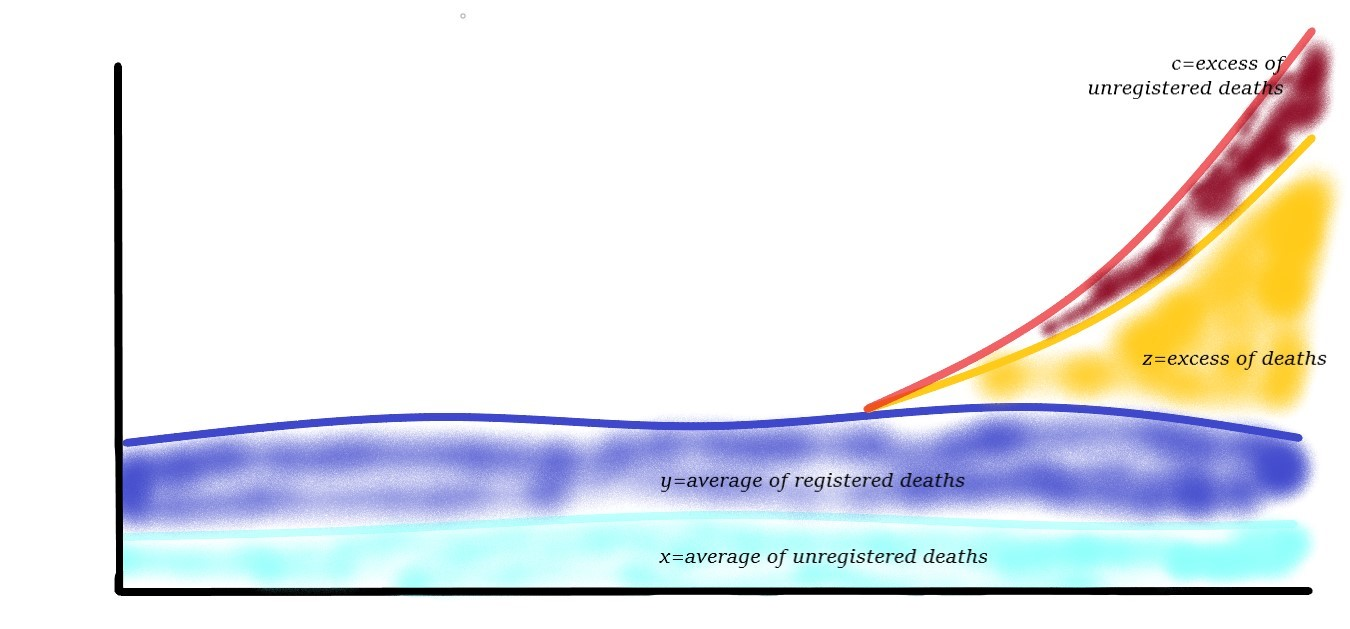
\includegraphics[width=1\linewidth]{C:/Users/LUCAS/Desktop/Excess.deaths.PERU/graph.excess} \caption{Understanding excess of mortality}\label{fig:excess}
\end{figure}

We compute excess deaths from an unobserved counterfactual scenario, which projects average weekly deaths from previous years to the present. This requires assessing the potential existence of differences between 2020 and previous years. In some cases there is visual evidence of a pattern change. In other cases, we need to implement more sophisticated tools to detect possible differences over time.

To do this, we fit a Bayesian state-space time series model (Scott and Varian 2014) using data prior to the pre-intervention and developing a conterfactual time series synthetic control (Abadie, Diamond, and Hainmueller 2010). The inferential part of the method relies on the use of Markov chain Monte Carlo (MCMC) to simulate the counterfactual posterior distribution. In this case, we compare the expected value of the observed data \(y_\text{t}\) in time points \(\text{t}=\text{t}_0+1+...,\text{t}\) to the average of samples from the forecasted posterior distribution \(\hat y_{t}\) of each draw \({\tau}\). More details about the method and the implementation packages \texttt{CausalImpact} and \texttt{BSTS} are found in (Brodersen et al. 2015; Scott and Varian 2014). Synthetic control methods have been widely used in the field (Bouttell et al. 2018), while this specific method has been already used to evaluate health interventions (Bruhn et al. 2017; Kurz et al. 2019).

In our case, we are looking to evaluate changes in the number of deaths registered since the outbreak of COVID-19. We state as our null hypothesis, \(H_0\) the absence of a significant change in the number of registered deaths during 2020 at the regional level, as:

\begin{equation}
  \label{eq:bayes}
   \begin{cases}
  H_0: \phi_{t}^{\tau}= y_{t} -  \hat y_{t}^{\tau} = 0 \\[1ex]
  H_a: \phi_{t}^{\tau}= y_{t} -  \hat y_{t}^{\tau} \neq 0.
   \end{cases}
\end{equation}

Now we turn to the computation of excess mortality for areas where there is robust evidence of excess deaths. Our approach decomposes the estimation of total excess of deaths \(\text{Excess.d}_\text{T}\) into two dimensions: one related to the registered death count and other related to the average and the additional non-registered deaths. The decomposition is:

\begin{equation}
  \label{eq:9}
  \widehat{\text{Excess.d}}_\text{T} = \widehat{\text{Excess.d}}_\text{Reg}+\widehat{\mu}_{\text{Deaths}_\text{Not.reg}}
\end{equation}

The computation of the first term of Equation \eqref{eq:9}, the excess of registered mortality, \(\widehat{\text{Excess.d}}_\text{Reg}\), is based only on data provided by SINADEF. We compare the weekly average of deaths from 2018 and 2019 to the number of weekly deaths in 2020. We compare values from mid-March, when the first COVID-19 death case was registered, until the current time. This can be formally notated as:

\begin{equation}
  \label{eq:10}
  \widehat{\text{Excess.d}}_\text{Reg}= \frac{1}{n}{\sum_{week=12}^{n} \text{Reg.deaths}_{2020}}-1/n{\sum_{week=12}^{n} \text{Reg.deaths}_{2017-2019}}
\end{equation}

The second term consists in the estimation of the recent historic average of not registered deaths in the country, \(\widehat{\mu}_{\text{Deaths}_\text{Not.reg}}\). T This relies on the assumption that under-registration in recent years is a reasonable counterfactual to estimate missing registration in 2020. We explore visual patterns and rates to evaluate the robustness of the assumption. We follow a deterministic approach and assume under-registered COVID-19 deaths are also captured in this term. The term is computed as the product of the registration completeness ratio, \(\widehat{\text{Comp.reg}}\) and the average of registered deaths on 2018-2019, \(\widehat{\text{Comp.reg}}\), as follows:

\begin{equation}
  \label{eq:11}
  \widehat{\mu}_{\text{Deaths}_\text{Not.reg}}= (1-\widehat{\text{Comp.reg}})*\widehat{\text{Excess.d}}_\text{Reg}
\end{equation}

We now address three cases of atypical data behaviour.

First, some regions of Peru may not be significantly affected by COVID-19. This case corresponds to the non rejection of \(H_0\) based on the hypothesis tests of \eqref{eq:bayes}. A second case occurs when there is no solid evidence suggesting under-registration of deaths over time in some regions or age groups, which is given by \(\widehat{\text{Excess.d}}_\text{Not.reg} \le 0\). This occurs usually in areas or sub-categories with very small populations. A third possibility is the scenario where less deaths occur due to a positive but unintended effect of quarantine or curfews (such as fewer road accidents or violent crimes). In this case, certain groups are not affected by an excess of deaths, and then \(\widehat{\text{Excess.d}}_\text{Reg} \le 0\). In these cases, we compute excess deaths without adding the terms from Equation \eqref{eq:11} referring to unregistered figures (as they would provide add negative values to the sum, biasing the results). To address uncertainty, we estimate the total excess deaths only computing a 95\% CI based on the standard error of the parameter, where \(\text{n}\) represents the number of observations at the regional level.

In the other cases, we compute the overall magnitude of mortality adding both terms. Equation \eqref{eq:13} summarises the estimation of \(\widehat{\text{Excess.d}}_\text{T}\) based on INEI data, where the 95\% CI are provided by prior estimations of lower and upper bounds from Equations \eqref{eq:4} and \eqref{eq:6}, conditionally to \eqref{eq:bayes} and \(\widehat{\text{Excess.d}}_\text{Reg} \le 0 \lor\widehat{\text{Excess.d}}_\text{Reg} \geq 0\). as follows:

\begin{equation} \label{eq:13}
      \begin{cases}
      \!\begin{aligned}
        & \widehat{\text{Excess.d}}_\text{T}= \widehat{\text{Excess.d}}_\text{Reg} 
        \pm 1.96\sqrt(\hat{\sigma}_\frac{{\text{Excess.d}}_\text{Reg}}{\text{n}-1}), 
        &\text{if }\phi(\tau)=0 \lor \widehat{\text{Excess.d}}_\text{Reg} \le 0,  \\[1ex]
        &\widehat{\text{Excess.d}}_{\text{T}_\text{max}} = \widehat{\text{Excess.d}}_\text{Reg}+
        \Big(\widehat{\mu}_{\text{Deaths}_\text{Not.reg}}+
        1.96\sqrt{\widehat{\text{MR}}*\widehat{\text{pop}}\sqrt{(\frac{\hat{\sigma}_\text{MR}}{\widehat{\text{MR}}})^2+
        (\frac{\hat{\sigma}_\text{pop}}{\widehat{\text{pop}}})^2}}\Big) & \text{and }\\[1ex]
        &\widehat{\text{Excess.d}}_{\text{T}_\text{min}} =  \widehat{\text{Excess.d}}_\text{Reg}+
        \Big(\widehat{\mu}_{\text{Deaths}_\text{Not.reg}}-
        1.96\sqrt{\widehat{\text{MR}}*\widehat{\text{pop}}\sqrt{(\frac{\hat{\sigma}_\text{MR}}{\widehat{\text{MR}}})^2+
        (\frac{\hat{\sigma}_\text{pop}}{\widehat{\text{pop}}})^2}}\Big),\\[1ex]
        &\text{if }\phi(\tau) \neq 0  \land \widehat{\text{Excess.d}}_\text{Reg} \geq 0.
    \end{aligned}
  \end{cases}
  \end{equation}

In case of GBD, total excess of mortality \(\widehat{\text{Excess.d}}_\text{T}\) and the 95\% CI are estimated from Equations \eqref{eq:4b} and \eqref{eq:9}, conditionally to \eqref{eq:bayes} as follows:

\begin{equation} \label{eq:14}
      \begin{cases}
      \!\begin{aligned}
        & \widehat{\text{Excess.d}}_\text{T}= \widehat{\text{Excess.d}}_\text{Reg} 
        \pm 1.96\sqrt{\hat{\sigma}_{\text{Excess.d}_\text{Reg}}},
        &\text{if }\phi(\tau)=0 \lor \widehat{\text{Excess.d}}_\text{Reg} \le 0,  \\%[1ex]
        &\widehat{\text{Excess.d}}_\text{T} = \widehat{\text{Excess.d}}_\text{Reg}+\widehat{\mu}_{\text{Deaths}_\text{Not.reg}}+\widehat{\text{Excess.d}}_\text{Not.reg} 
        &\text{and }\\[1ex]
        &\widehat{\text{Excess.d}}_{\text{T}_\text{max}} = \widehat{\text{Excess.d}}_\text{Reg}+
        \Big( \widehat{\mu}_{\text{Deaths}_\text{Not.reg}}+
        1.96\sqrt{\hat{\sigma}_{\text{Excess.d}_\text{Reg}}} \Big)  &\text{and }\\[1ex]
              &\widehat{\text{Excess.d}}_{\text{T}_\text{min}} = \widehat{\text{Excess.d}}_\text{Reg}+
        \Big (\widehat{\mu}_{\text{Deaths}_\text{Not.reg}}-
        1.96\sqrt{\hat{\sigma}_{\text{Excess.d}_\text{Reg}}} \Big), &\text{if }\phi(\tau) \neq 0  \land \widehat{\text{Excess.d}}_\text{Reg} \geq 0.
    \end{aligned}
  \end{cases}
  \end{equation}

Our analysis makes two assumptions. First, it analysis assumes that comparison between years is not invalidated by specific time-bound mortality events such as additional disease outbreaks or wars. A second assumption is that registration patterns remain stable and any changes over time are due to death rates. Both assumptions can be assessed by visualising the data and analysing changing trends. More complex analysis such as change-point detection, computing growth rates or advanced time series analysis could also be valuable, although the absence of stationary data cannot be easily solved without in-depth knowledge of real causes.
We use SINADEF data for 2018 to 2020 but not for 2017. First, as a new system, the magnitude of data collected is not stable in comparison to other years. In case of Lambayeque, after visually and analytically assessing a significant change in trend in 2020, we only use data from 2019 and 2020, as the inclusion of the prior year on the average distorts results for some subgroups, resulting in negative excess mortality.

\hypertarget{step-2-results}{%
\subsubsection{Step 2: Results}\label{step-2-results}}

We plot the time series of SINADEF by region to visually assess if our assumptions hold. Figure \ref{fig:patterns} shows almost all regions present a stable trend over time, with negative peaks at the end of each year (around weeks 53, 106, 154) due to interrupted reporting during national holidays. A few regions such as Lima, Cusco and Arequipa show a slight increase from 2017, due to their large populations compared to other regions, which is expected to create a clearer learning curve in terms of adherence to the new system. By 2020, most regions show significant increases in deaths. The vertical orange line shows the week for the first confirmed COVID-19 death. Four regions provide no evidence of COVID-19 deaths: Ayacucho, Cusco, Puno and Tacna. Lambayeque shows a very erratic trend through 2019, which suddenly changes at the beginning of the pandemic in mid-March.

\begin{figure}
\centering
\includegraphics{tutorial3final_files/figure-latex/patterns-1.pdf}
\caption{\label{fig:patterns}Weekly deaths by region registered in SINADEF}
\end{figure}

\hypertarget{weekly-deaths-by-region-registered-in-sinadef}{%
\paragraph{Weekly deaths by region registered in SINADEF}\label{weekly-deaths-by-region-registered-in-sinadef}}

To assess whether there has been a change of patterns, we perform a Bayesian Times series univariate analysis on weekly averages from week 2 (avoiding the seasonal under-reporting of week 1) to week 28 of 2020. We set week 16 as the cut-off point, which is three weeks later than the first registered death by COVID-19 in the country. This relies on observed data that the spread of COVID-19 across regions was uneven. We draw MCMC 5,000 samples to increase the accuracy of inference and set a Bayesian one-sided tail-area probability p \textless. 05 to reject \(H_0\). Table \ref{tab:cac1} shows only Puno present p.\textgreater.05 and it will be excluded from the estimates of excess of mortality (as they may provide positive values that bias the final estimates). This case will receive a different treatment, as stated in Equations \eqref{eq:13} and \eqref{eq:14}.

\begin{table}[!h]

\caption{\label{tab:cac1}Average of predicted deaths under Bayesian Time Series Analysis counterfactual estimation and significance tests}
\centering
\begin{tabular}[t]{lrrrrr}
\toprule
Departamento & Pred & Pred.lower & Pred.upper & Pred.sd & p\\
\midrule
AMAZONAS & 7.1015316 & 2.260177 & 11.951297 & 2.465145 & 0.0002008\\
ANCASH & 99.8941089 & 88.870161 & 111.121816 & 5.704213 & 0.0002002\\
APURIMAC & 28.4900685 & 20.384792 & 36.804274 & 4.195315 & 0.0232932\\
AREQUIPA & 112.6800115 & 90.211598 & 135.371305 & 11.578070 & 0.0002000\\
AYACUCHO & 10.1242816 & 0.547666 & 19.934549 & 4.963521 & 0.0002000\\
\addlinespace
CAJAMARCA & 41.1034224 & 32.533619 & 49.754380 & 4.371634 & 0.0002000\\
CALLAO & 103.9850479 & 90.541118 & 118.015579 & 7.105448 & 0.0002000\\
CUSCO & 70.8261649 & 58.890741 & 83.409814 & 6.317878 & 0.0002008\\
HUANCAVELICA & 34.3933787 & 26.140355 & 42.664821 & 4.233648 & 0.0438000\\
HUANUCO & 46.2989879 & 38.514061 & 54.144275 & 3.956012 & 0.0002006\\
\addlinespace
ICA & 68.9795616 & 56.825611 & 81.024259 & 6.190525 & 0.0002000\\
JUNIN & 105.0365438 & 92.082474 & 118.070088 & 6.626338 & 0.0002002\\
LA LIBERTAD & 86.9884047 & 68.792908 & 105.796931 & 9.429550 & 0.0002009\\
LAMBAYEQUE & 17.9117845 & 10.644342 & 25.249844 & 3.718587 & 0.0002002\\
LIMA & 1026.5074242 & 941.287186 & 1112.218121 & 43.675649 & 0.0002002\\
\addlinespace
LORETO & 33.0271116 & 24.030397 & 42.455007 & 4.683722 & 0.0002000\\
MADRE DE DIOS & 0.9805459 & -4.673200 & 6.671235 & 2.892826 & 0.0002009\\
MOQUEGUA & 7.0372713 & 2.451331 & 11.703004 & 2.362294 & 0.0002000\\
PASCO & 10.9370637 & 5.343668 & 16.654026 & 2.879414 & 0.0008024\\
PIURA & 66.9194108 & 54.110030 & 79.823199 & 6.495689 & 0.0002006\\
\addlinespace
PUNO & 75.2992563 & 60.155543 & 90.907603 & 7.807562 & 0.3608826\\
SAN MARTIN & 27.3370412 & 18.008682 & 36.874402 & 4.866695 & 0.0002009\\
TACNA & 8.1267233 & 2.514384 & 13.707266 & 2.883408 & 0.0006008\\
TUMBES & 17.6133287 & 12.915063 & 22.217275 & 2.371243 & 0.0002006\\
UCAYALI & 31.1195139 & 22.562714 & 40.063186 & 4.470999 & 0.0002002\\
\bottomrule
\end{tabular}
\end{table}

With reference to age, Figure \ref{fig:sinadefrange} similar patterns across all groups, following the population-wide results of stable trends with negative yearly peaks. The effect of the pandemics is clear across older cohorts, while the opposite applies for younger ages. In some groups, such as people aged 20-39, there is a delayed negative effect of the pandemic. The last plot of the series reflects cases without an age identification and thus represent white noise (NA). They have a very small y-scale and they do not affect the overall trends.

\begin{figure}
\centering
\includegraphics{tutorial3final_files/figure-latex/sinadefrange-1.pdf}
\caption{\label{fig:sinadefrange}Weekly deaths by range of age registered in SINADEF}
\end{figure}

We decompose regional data into different components: seasonal patterns, trend and residual components using locally estimated scatterplot smoothing (LOESS). This enables us to identify specific seasonal effects (Robert B Cleveland et al. 1990). We set a periodic window that assumes no major changes in patterns over the last three years and apply robust smoothing to deal with possible data outliers. Figure \ref{fig:STL} shows the results of the decomposition exercise for one region, Cusco. It shows both a strong influence of long-term trends and the absence of weekly seasonality. The same pattern is found in all other regions. Model parameters are found in the Appendix.

\begin{figure}[H]

{\centering \includegraphics{tutorial3final_files/figure-latex/STL-1} 

}

\caption{STL decomposition - CUSCO}\label{fig:STL}
\end{figure}

The estimations of excess of registered deaths based on SINADEF raises to 41,700 deaths by week 28 (ending 12.7.20). Table \ref{tab:excessreg} presents excess deaths disaggregated by regions. Lima has the highest excess with 24,397 deaths over the previous average, followed by Callao and Piura (3,083 and 2,612). Some regions (Amazonas, Ayacucho, Cajamarca, Cusco, Puno and Tacna, among others) have negative excess mortality. This will affect the final computation strategy, as mentioned above. The region of Puno reports the largest positive scenario with 468 fewer deaths than the average over previous years, followed by Cusco (338).

\begin{table}[!h]

\caption{\label{tab:excessreg}Excess of deaths based on SINADEF - weeks 12 to 28 in 2020 by regions}
\centering
\begin{tabular}[t]{lr}
\toprule
Departamento & s\\
\midrule
AMAZONAS & -12.0\\
ANCASH & 1484.0\\
APURIMAC & 105.5\\
AREQUIPA & 1549.0\\
AYACUCHO & -181.0\\
\addlinespace
CAJAMARCA & -52.0\\
CALLAO & 3083.0\\
CUSCO & -338.0\\
HUANCAVELICA & 49.0\\
HUANUCO & 182.5\\
\addlinespace
ICA & 1707.0\\
JUNIN & 483.5\\
LA LIBERTAD & 2371.5\\
LAMBAYEQUE & 1305.0\\
LIMA & 24397.0\\
\addlinespace
LORETO & 1353.0\\
MADRE DE DIOS & 165.0\\
MOQUEGUA & 40.5\\
PASCO & 118.5\\
PIURA & 2612.5\\
\addlinespace
PUNO & -468.0\\
SAN MARTIN & 416.0\\
TACNA & -133.5\\
TUMBES & 536.0\\
UCAYALI & 925.5\\
\bottomrule
\end{tabular}
\end{table}

Table \ref{tab:excessage} shows excess mortality for age groups. Deaths among people aged up to 30 are below average. By contrast, excess mortality for people aged 60 or over surpasses 10,000.

\begin{table}[!h]

\caption{\label{tab:excessage}Excess of deaths based on SINADEF - weeks 12 to 28 in 2020 by regions}
\centering
\begin{tabular}[t]{lr}
\toprule
range & s\\
\midrule
a0.9 & -690.5\\
a10.19 & -24.0\\
a20.29 & -47.5\\
a30.39 & 760.0\\
a40.49 & 2913.0\\
\addlinespace
a50.59 & 6902.0\\
a60.69 & 11328.0\\
a70.79 & 10719.0\\
a80 & 9839.5\\
\bottomrule
\end{tabular}
\end{table}

Combined analysis of SINADEF and reported COVID-19 deaths shows an important gap for all regions with excess mortality. Figure \ref{fig:excessCOVID} shows that Lima, Callao, Piura, Ucayali, Loreto, and Tumbes have over double the number of deaths compared to previous years. In Lambayeque COVID-19 deaths make up 50.6\% of total mortality, while in Lima and Piura they make up 15.8\% and 18.6\%. This may mean that reporting of deaths not caused by COVID-19 is relatively low in Lambayeque or that Lima and Piura are reporting a lower share of deaths caused by COVID-19. Since it is unsafe to assume stable reporting for the region of Lambayeque, we compare 2020 weeks against values in 2017 in the final analysis. This gives a better estimate for the expected number of registered deaths.

\begin{center}\includegraphics{tutorial3final_files/figure-latex/excessCOVID-1} \end{center}

We now present our estimate of total excess deaths, which include the non-registered terms in the equation. The estimates consider different scenarios, using INEI and GBD mortality and population projections, and fitting data using the \(\text{ARIMA}\) and \(\text{RWD}\) models.

Table \ref{tab:exinei} summarises aggregated estimates, with mean values of around 54,600 deaths for all the regressions. For example, the combination of \(\text{ARIMA}\) models gives an expected value of 54,645 95\% CI (45,534 to 63,739). This clearly suggests a significant downward bias of identification of COVID-19 deaths in official sources(reporting 12,504 deaths). Estimated non-registered notifications add 13,000 to excess registered mortality (equivalent to 23.7\% of non-registered deaths). This level of underestimate is slightly higher than for the GBD estimates (Dicker et al. 2018), which generate around 19.6\% additional deaths. Comparing death registrations from INEI and SINADEF in 2016 and 2017 shows SINADEF registrations still lag behind previous years.

\begin{table}[!h]

\caption{\label{tab:exinei}Estimated of excess of deaths based on INEI - weeks 12 to 28}
\centering
\begin{tabular}[t]{llrrrrr}
\toprule
model.pop & model.mort & Total excess & Lower.CI95\% & Upper.CI95\% & Deaths SINADEF & Covid deaths\\
\midrule
arima & arima & 54644.80 & 45533.42 & 63738.39 & 78624 & 8586\\
arima & drift & 54866.65 & 45727.64 & 63984.48 & 78624 & 8586\\
drift & arima & 54712.03 & 45603.95 & 63802.61 & 78624 & 8586\\
drift & drift & 54941.02 & 45805.67 & 64055.56 & 78624 & 8586\\
\bottomrule
\end{tabular}
\end{table}

Table \ref{tab:exineiage} shows that 76\% of total excess deaths are among people aged 60 or over, with an expected value of 42,000 additional deaths across the models. For people 80 or over reported COVID-19 deaths account for the lowest share of total estimated excess deaths (15.9\%), possible due to higher rates of misreporting cause of death for this age group.

\begin{table}[!h]

\caption{\label{tab:exineiage}Estimated of excess of deaths based on INEI - weeks 12 to 28: age groups}
\centering
\begin{tabular}[t]{lrrrrrr}
\toprule
range & Excess & Lower.CI & Upper.CI & SINADEF & Covid & Covid:Excess\\
\midrule
a0.9 & -683.84937 & -4212.0421 & 2844.285 & 1446 & 25 & -0.0365578\\
a10.19 & -12.87355 & -3000.6521 & 2974.784 & 583 & 17 & -1.3205369\\
a20.29 & -19.99634 & -1345.9894 & 1305.855 & 1204 & 73 & -3.6506677\\
a30.39 & 1003.55196 & 824.2866 & 1181.999 & 2421 & 250 & 0.2491152\\
a40.49 & 3802.84215 & 3648.9058 & 3954.323 & 5205 & 700 & 0.1840729\\
\addlinespace
a50.59 & 9058.84391 & 8874.8965 & 9238.502 & 10386 & 1606 & 0.1772853\\
a60.69 & 14889.54887 & 14686.6907 & 15087.655 & 16409 & 2428 & 0.1630674\\
a70.79 & 13982.86757 & 13792.9600 & 14169.433 & 18075 & 2097 & 0.1499692\\
a80 & 12623.86828 & 12264.3681 & 12981.550 & 22895 & 1390 & 0.1101089\\
\bottomrule
\end{tabular}
\end{table}

Table \ref{tab:exineiregion} presents estimations of excess of deaths by region. Lima shows 29,309 95\% CI (25760, 32857) deaths followed by Callao, Piura, Lambayeque and La Libertad, averaging 2,500 to 3,100 deaths. Six regions yield negative values: Amazonas, Ayacucho, Cajamarca, Cusco, Puno and Tacna. However, in cases like Amazonas, Ayacucho and Tacna the upper bound of 95\% are close or over 0.

Table \ref{tab:exineiregion} shows estimated excess deaths by region. For Lima there were 31,933 95\% CI (28,077, 35,786) excess deaths, followed by Callao, Piura, Lambayeque and La Libertad, averaging 2,500 to 3,100 deaths. Four regions yield negative expected values: Ayacucho, Cusco, Puno and Tacna. In cases like Amazonas and Cajamarca the lower levels of the 95\% CI are lower than 0.

\begin{table}[!h]

\caption{\label{tab:exineiregion}Estimated of excess of deaths based on INEI - weeks 12 to 28: regions}
\centering
\begin{tabular}[t]{lrrrrr}
\toprule
Departamento & Total excess & Lower.CI95\% & Upper.CI95\% & Deaths SINADEF & Covid deaths\\
\midrule
AMAZONAS & 5.679648 & -50.47077 & 61.79354 & 279 & 34\\
ANCASH & 1868.131371 & 1595.76289 & 2139.16577 & 3277 & 437\\
APURIMAC & 155.583989 & 97.76301 & 213.35216 & 587 & 14\\
AREQUIPA & 1613.198315 & 1315.77771 & 1909.63284 & 3553 & 203\\
AYACUCHO & -181.000000 & -375.83894 & 13.83894 & 472 & 21\\
\addlinespace
CAJAMARCA & 8.264441 & -136.97967 & 153.45506 & 1097 & 24\\
CALLAO & 3352.695019 & 2577.55135 & 4125.93972 & 4515 & 563\\
CUSCO & -334.137683 & -508.85412 & -159.43866 & 1723 & 13\\
HUANCAVELICA & 71.546043 & 44.87256 & 97.93794 & 687 & 10\\
HUANUCO & 287.840845 & 224.49392 & 351.04312 & 1136 & 47\\
\addlinespace
ICA & 1501.554288 & 1198.92541 & 1801.78014 & 3104 & 433\\
JUNIN & 654.940015 & 509.83833 & 799.69506 & 2403 & 116\\
LA LIBERTAD & 2863.842721 & 2226.64696 & 3499.76514 & 4927 & 496\\
LAMBAYEQUE & 2594.687652 & 1986.99107 & 3202.28350 & 2856 & 718\\
LIMA & 31932.512306 & 28077.89874 & 35786.12689 & 35182 & 3950\\
\addlinespace
LORETO & 2209.635656 & 2082.70799 & 2335.58950 & 2032 & 332\\
MADRE DE DIOS & 181.159976 & 124.63632 & 235.08053 & 392 & 24\\
MOQUEGUA & 47.450977 & 40.95871 & 53.71032 & 284 & 9\\
PASCO & 200.045641 & 179.24623 & 220.63487 & 343 & 20\\
PIURA & 3740.486752 & 3090.87961 & 4389.44053 & 4524 & 715\\
\addlinespace
PUNO & -468.000000 & -801.95217 & -134.04783 & 1321 & 16\\
SAN MARTIN & 604.674970 & 530.66790 & 678.47160 & 1268 & 126\\
TACNA & -133.001306 & -212.58624 & -53.45341 & 282 & 8\\
TUMBES & 594.991855 & 528.17644 & 659.39315 & 859 & 112\\
UCAYALI & 1272.019979 & 1186.31090 & 1357.19540 & 1521 & 145\\
\bottomrule
\end{tabular}
\end{table}

Table \ref{tab:exgbd} shows estimates based on GBD data, which, at around 46,000, are slightly lower than those based on INEI data. Confidence intervals are significantly larger than for the models based on INEI data, signifying a 19\% under-registration rate. Estimations show same patterns than INEI models across age groups, with 75\% of excess deaths occurring among people aged 60 and Lima, Piura and Callao reporting the largest shares of deaths.

\begin{table}[!h]

\caption{\label{tab:exgbd}Estimated of excess of deaths based on GBD - weeks 12 to 28}
\centering
\begin{tabular}[t]{lrrrrr}
\toprule
.model & Total excess & Lower.CI95\% & Upper.CI95\% & Deaths SINAEF & Covid deaths\\
\midrule
arima & 51188.24 & 40057.27 & 62019.83 & 78624 & 8586\\
drift & 51713.74 & 40697.12 & 62446.05 & 78624 & 8586\\
\bottomrule
\end{tabular}
\end{table}

Figure \ref{fig:ex} shows estimates by region and age group. The general trend is for higher rates of excess deaths among older people, although this is not the case for some regions Ayacucho, Cajamarca, Moquegua and Tacna. The reasons for this counter-intuitive result are not explored in this paper.

\begin{figure}[H]

{\centering \includegraphics{tutorial3final_files/figure-latex/ex-1} 

}

\caption{Total excess of deaths by regions - different models}\label{fig:ex}
\end{figure}

Table \ref{tab:compare} shows projections based on current excess deaths, assuming all other things remain equal. This shows an increase to 195,000 expected deaths, which is 21.7 \% higher than INEI estimates for 2020.

\begin{table}[!h]

\caption{\label{tab:compare}Projected number of deaths Estimated of excess of deaths based on GBD - weeks 12 to 28}
\centering
\begin{tabular}[t]{llrr}
\toprule
model.pop & model.mort & Ratio Excess & Projected 2020\\
\midrule
arima & arima & 0.7631009 & 195025.3\\
arima & drift & 0.7600154 & 195817.1\\
drift & arima & 0.7621632 & 195265.3\\
drift & drift & 0.7589866 & 196082.5\\
\bottomrule
\end{tabular}
\end{table}

Our comparisons across results need to take into account differences in population sizes and age structures. To address this problem, we compute standardised adjusted mortality rates across regions using direct standardisation (Curtin and Klein 1995). We use population estimates by region and age group, as well as total estimated deaths. Table \ref{tab:smrd} shows adjusted mortality ratios by region until week 28 of 2020. Ucayali, Tumbes, Madre de Dios, Loreto and Callao have rates of over 4, while Puno, Amazonas, Tacna and Ayacucho show the lowest adjusted rates -less than 1.

\begin{table}[!h]

\caption{\label{tab:smrd}Age standardised mortality rates by regions 2020 - up to week 28}
\centering
\begin{tabular}[t]{lr}
\toprule
Departamento & std.d\\
\midrule
AMAZONAS & 0.9099395\\
ANCASH & 3.3827087\\
APURIMAC & 2.0884530\\
AREQUIPA & 2.3462059\\
AYACUCHO & 0.8513508\\
\addlinespace
CAJAMARCA & 1.1206732\\
CALLAO & 4.0117474\\
CUSCO & 1.3960288\\
HUANCAVELICA & 2.4557700\\
HUANUCO & 2.1443842\\
\addlinespace
ICA & 3.1431579\\
JUNIN & 2.4831039\\
LA LIBERTAD & 3.0124320\\
LAMBAYEQUE & 3.4998962\\
LIMA & 3.9156776\\
\addlinespace
LORETO & 4.2204854\\
MADRE DE DIOS & 4.3573846\\
MOQUEGUA & 1.4774693\\
PASCO & 2.3053489\\
PIURA & 3.6591048\\
\addlinespace
PUNO & 0.9561755\\
SAN MARTIN & 2.7730377\\
TACNA & 0.8711758\\
TUMBES & 4.7830820\\
UCAYALI & 4.8830833\\
\bottomrule
\end{tabular}
\end{table}

\hypertarget{conclusion}{%
\section{Conclusion}\label{conclusion}}

This tutorial and case study provides a framework and tools to estimate the burden of death caused by the COVID-19 pandemic. This tutorial sets out an analytical path for progressively gathering and analyzing information to generate robust estimates of excess mortality. This approach can be applied in all countries, although the complexity of analysis will vary according to the availability and accuracy of data. There is strong evidence that excess COVID-19 mortality has disproportionately affected people at older ages (Dowd et al. 2020). Consequently, we include population age structure in our analysis.

The case of Peru shows that significant under-registration of deaths caused by COVID-19. Official figures correspond to only 20-22\% of total excess mortality and registered deaths. Different models and databases show that Lima, Piura, Callao are the worst affected regions and people 60 and over the most affected age group. Adjusted analysis shows that excess mortality is higher in less populated regions such as Tumbes and the amazon states of Ucayali, Loreto and Madre de Dios. Some regions, especially in the Andes, do not appear to have been significantly affected by the pandemic by the end of June, in terms of mortality.

There are important limitations in our method. Estimates are based on provisional data, which are incomplete. Our estimates of registration completeness assume no variation across age groups, which may not be the case. Our time series analysis produces higher CIs when forecasting over extended periods, reducing the precision of estimates. Lags in reporting deaths may reduce the validity of our cutoffs. Finally, we present a conservative scenario, allowing for the existence of negative as well as positive excess deaths.

\hypertarget{Appendix}{%
\section{Appendix}\label{Appendix}}

\hypertarget{model-fit-and-residuals-analysis-population-inei}{%
\subsubsection{Model fit and residuals analysis: population INEI}\label{model-fit-and-residuals-analysis-population-inei}}

\begin{table}[!h]

\caption{\label{tab:fite}Model fit population INEI}
\centering
\begin{tabular}[t]{llllrrrr}
\toprule
Departamento & range & .model & term & estimate & std.error & statistic & p.value\\
\midrule
AMAZONAS & a0.9 & arima & ar1 & 2.757741e+00 & 0.2627990 & 1.049373e+01 & 0.0000005\\
AMAZONAS & a0.9 & arima & ar2 & -2.546586e+00 & 0.5386097 & -4.728073e+00 & 0.0006213\\
AMAZONAS & a0.9 & arima & ar3 & 7.869771e-01 & 0.2795229 & 2.815430e+00 & 0.0168045\\
AMAZONAS & a0.9 & arima & ma1 & 6.571431e-01 & 0.4755400 & 1.381888e+00 & 0.1944245\\
AMAZONAS & a0.9 & arima & constant & 1.431607e+02 & 98.6818444 & 1.450730e+00 & 0.1747666\\
\addlinespace
AMAZONAS & a10.19 & arima & ar1 & 2.720592e+00 & 0.0978614 & 2.780046e+01 & 0.0000000\\
AMAZONAS & a10.19 & arima & ar2 & -2.621606e+00 & 0.1850259 & -1.416886e+01 & 0.0000000\\
AMAZONAS & a10.19 & arima & ar3 & 8.904879e-01 & 0.1032087 & 8.628033e+00 & 0.0000032\\
AMAZONAS & a10.19 & arima & constant & 8.473559e+02 & 34.2248245 & 2.475852e+01 & 0.0000000\\
AMAZONAS & a20.29 & arima & ar1 & 2.610032e+00 & 0.2135079 & 1.222452e+01 & 0.0000001\\
\addlinespace
AMAZONAS & a20.29 & arima & ar2 & -2.445307e+00 & 0.3892194 & -6.282593e+00 & 0.0000598\\
AMAZONAS & a20.29 & arima & ar3 & 8.043516e-01 & 0.2157773 & 3.727692e+00 & 0.0033368\\
AMAZONAS & a20.29 & arima & ma1 & 6.691210e-01 & 0.3768175 & 1.775717e+00 & 0.1034150\\
AMAZONAS & a20.29 & arima & constant & 2.290744e+03 & 41.0057408 & 5.586399e+01 & 0.0000000\\
AMAZONAS & a30.39 & arima & ar1 & 8.317636e-01 & 0.1512684 & 5.498596e+00 & 0.0002623\\
\addlinespace
AMAZONAS & a30.39 & arima & constant & 1.457050e+02 & 27.0185076 & 5.392784e+00 & 0.0003045\\
AMAZONAS & a40.49 & arima & ar1 & 7.939404e-01 & 0.1732111 & 4.583658e+00 & 0.0010050\\
AMAZONAS & a40.49 & arima & constant & 2.568133e+02 & 12.6877334 & 2.024107e+01 & 0.0000000\\
AMAZONAS & a50.59 & arima & constant & 8.735000e+02 & 38.1774954 & 2.287997e+01 & 0.0000000\\
AMAZONAS & a60.69 & arima & ar1 & 1.875195e+00 & 0.0315923 & 5.935602e+01 & 0.0000000\\
\addlinespace
AMAZONAS & a60.69 & arima & ar2 & -9.750777e-01 & 0.0289986 & -3.362496e+01 & 0.0000000\\
AMAZONAS & a60.69 & arima & ma1 & 3.717597e-01 & 0.2475209 & 1.501933e+00 & 0.1640153\\
AMAZONAS & a60.69 & arima & constant & 4.692915e+01 & 2.8774274 & 1.630941e+01 & 0.0000000\\
AMAZONAS & a70.79 & arima & ar1 & 1.622911e+00 & 0.1073952 & 1.511159e+01 & 0.0000000\\
AMAZONAS & a70.79 & arima & ar2 & -9.184459e-01 & 0.0965296 & -9.514653e+00 & 0.0000025\\
\addlinespace
AMAZONAS & a70.79 & arima & ma1 & 8.111050e-02 & 0.4141343 & 1.958556e-01 & 0.8486458\\
AMAZONAS & a70.79 & arima & constant & 7.240616e+01 & 2.6012649 & 2.783498e+01 & 0.0000000\\
AMAZONAS & a80 & arima & ar1 & 1.862031e+00 & 0.0332592 & 5.598547e+01 & 0.0000000\\
AMAZONAS & a80 & arima & ar2 & -9.761466e-01 & 0.0257886 & -3.785192e+01 & 0.0000000\\
AMAZONAS & a80 & arima & constant & 1.164520e+01 & 0.8047098 & 1.447130e+01 & 0.0000000\\
\addlinespace
ANCASH & a0.9 & arima & constant & -1.508800e+03 & 40.2320031 & -3.750248e+01 & 0.0000000\\
ANCASH & a10.19 & arima & ar1 & 1.827095e+00 & 0.1202178 & 1.519821e+01 & 0.0000000\\
ANCASH & a10.19 & arima & ar2 & -8.828519e-01 & 0.1263681 & -6.986350e+00 & 0.0000378\\
ANCASH & a20.29 & arima & ar1 & 1.846786e+00 & 0.0787111 & 2.346284e+01 & 0.0000000\\
ANCASH & a20.29 & arima & ar2 & -9.246935e-01 & 0.0802366 & -1.152459e+01 & 0.0000004\\
\addlinespace
ANCASH & a30.39 & arima & constant & 1.199100e+03 & 104.3135426 & 1.149515e+01 & 0.0000004\\
ANCASH & a40.49 & arima & ar1 & 7.713430e-01 & 0.1799327 & 4.286842e+00 & 0.0015941\\
ANCASH & a40.49 & arima & constant & 5.768922e+02 & 34.2109630 & 1.686279e+01 & 0.0000000\\
ANCASH & a50.59 & arima & constant & 1.860000e+03 & 111.4704427 & 1.668604e+01 & 0.0000000\\
ANCASH & a60.69 & arima & ar1 & 1.872541e+00 & 0.0289375 & 6.470977e+01 & 0.0000000\\
\addlinespace
ANCASH & a60.69 & arima & ar2 & -9.625976e-01 & NaN & NaN & NaN\\
ANCASH & a60.69 & arima & ma1 & 7.075156e-01 & NaN & NaN & NaN\\
ANCASH & a60.69 & arima & constant & 9.366286e+01 & 6.3929997 & 1.465085e+01 & 0.0000000\\
ANCASH & a70.79 & arima & ar1 & 1.776352e+00 & 0.1637284 & 1.084938e+01 & 0.0000007\\
ANCASH & a70.79 & arima & ar2 & -7.811910e-01 & 0.1657812 & -4.712180e+00 & 0.0008262\\
\addlinespace
ANCASH & a80 & arima & ar1 & 1.941881e+00 & NaN & NaN & NaN\\
ANCASH & a80 & arima & ar2 & -9.450035e-01 & NaN & NaN & NaN\\
ANCASH & a80 & arima & ma1 & 8.640383e-01 & 0.2973579 & 2.905719e+00 & 0.0156793\\
APURIMAC & a0.9 & arima & constant & 1.036136e+05 & 217.5796192 & 4.762102e+02 & 0.0000000\\
APURIMAC & a10.19 & arima & ar1 & 1.964042e+00 & NaN & NaN & NaN\\
\addlinespace
APURIMAC & a10.19 & arima & ar2 & -9.654890e-01 & NaN & NaN & NaN\\
APURIMAC & a10.19 & arima & constant & 1.685135e+02 & NaN & NaN & NaN\\
APURIMAC & a20.29 & arima & ar1 & 2.562937e+00 & 0.1958369 & 1.308710e+01 & 0.0000000\\
APURIMAC & a20.29 & arima & ar2 & -2.337734e+00 & 0.3671667 & -6.366954e+00 & 0.0000532\\
APURIMAC & a20.29 & arima & ar3 & 7.339003e-01 & 0.2041788 & 3.594400e+00 & 0.0042110\\
\addlinespace
APURIMAC & a20.29 & arima & constant & 3.196645e+03 & 47.2466747 & 6.765863e+01 & 0.0000000\\
APURIMAC & a30.39 & arima & constant & 1.092400e+03 & 69.8552705 & 1.563805e+01 & 0.0000000\\
APURIMAC & a40.49 & arima & ar1 & 1.744020e+00 & 0.2088324 & 8.351293e+00 & 0.0000081\\
APURIMAC & a40.49 & arima & ar2 & -7.832334e-01 & 0.2191560 & -3.573862e+00 & 0.0050631\\
APURIMAC & a40.49 & arima & ma1 & 1.209952e+00 & 0.5991842 & 2.019332e+00 & 0.0710595\\
\addlinespace
APURIMAC & a40.49 & arima & ma2 & 3.652649e-01 & 0.3435270 & 1.063279e+00 & 0.3126574\\
APURIMAC & a50.59 & arima & ar1 & 8.746388e-01 & 0.1612462 & 5.424243e+00 & 0.0002913\\
APURIMAC & a50.59 & arima & constant & 5.770572e+01 & 8.2210409 & 7.019272e+00 & 0.0000363\\
APURIMAC & a60.69 & arima & ar1 & 9.850643e-01 & 0.0212564 & 4.634191e+01 & 0.0000000\\
APURIMAC & a70.79 & arima & ar1 & 1.847122e+00 & 0.1138654 & 1.622199e+01 & 0.0000000\\
\addlinespace
APURIMAC & a70.79 & arima & ar2 & -9.222472e-01 & 0.0911744 & -1.011520e+01 & 0.0000014\\
APURIMAC & a70.79 & arima & ma1 & 3.375335e-01 & 0.3469656 & 9.728156e-01 & 0.3535882\\
APURIMAC & a70.79 & arima & constant & 1.465085e+01 & 2.9391332 & 4.984750e+00 & 0.0005496\\
APURIMAC & a80 & arima & ar1 & 9.277940e-01 & 0.0981204 & 9.455669e+00 & 0.0000057\\
AREQUIPA & a0.9 & arima & ar1 & 2.742899e+00 & 0.1103504 & 2.485626e+01 & 0.0000000\\
\addlinespace
AREQUIPA & a0.9 & arima & ar2 & -2.615760e+00 & 0.2168307 & -1.206361e+01 & 0.0000001\\
AREQUIPA & a0.9 & arima & ar3 & 8.646905e-01 & 0.1182412 & 7.312938e+00 & 0.0000152\\
AREQUIPA & a0.9 & arima & constant & 1.712141e+03 & 11.2134389 & 1.526865e+02 & 0.0000000\\
AREQUIPA & a10.19 & arima & ar1 & 1.977165e+00 & 0.0287233 & 6.883494e+01 & 0.0000000\\
AREQUIPA & a10.19 & arima & ar2 & -9.776081e-01 & 0.0287158 & -3.404425e+01 & 0.0000000\\
\addlinespace
AREQUIPA & a20.29 & arima & ar1 & 1.894934e+00 & 0.0779339 & 2.431463e+01 & 0.0000000\\
AREQUIPA & a20.29 & arima & ar2 & -9.220533e-01 & 0.0740597 & -1.245014e+01 & 0.0000001\\
AREQUIPA & a20.29 & arima & constant & 6.008616e+03 & 72.1351129 & 8.329669e+01 & 0.0000000\\
AREQUIPA & a30.39 & arima & ar1 & 1.949861e+00 & 0.0336413 & 5.796032e+01 & 0.0000000\\
AREQUIPA & a30.39 & arima & ar2 & -9.696370e-01 & 0.0358596 & -2.703983e+01 & 0.0000000\\
\addlinespace
AREQUIPA & a40.49 & arima & ar1 & 1.706833e+00 & 0.0894859 & 1.907377e+01 & 0.0000000\\
AREQUIPA & a40.49 & arima & ar2 & -9.285108e-01 & 0.0800834 & -1.159429e+01 & 0.0000004\\
AREQUIPA & a40.49 & arima & ma1 & 4.774872e-01 & 0.4512998 & 1.058027e+00 & 0.3149313\\
AREQUIPA & a40.49 & arima & constant & 6.807557e+02 & 35.6824512 & 1.907816e+01 & 0.0000000\\
AREQUIPA & a50.59 & arima & ar1 & 1.767363e+00 & 0.0676104 & 2.614038e+01 & 0.0000000\\
\addlinespace
AREQUIPA & a50.59 & arima & ar2 & -9.417759e-01 & 0.0637257 & -1.477859e+01 & 0.0000000\\
AREQUIPA & a50.59 & arima & ma1 & 8.574872e-01 & 0.7127541 & 1.203062e+00 & 0.2566614\\
AREQUIPA & a50.59 & arima & constant & 5.973115e+02 & 20.1639972 & 2.962267e+01 & 0.0000000\\
AREQUIPA & a60.69 & arima & ar1 & 2.354777e+00 & NaN & NaN & NaN\\
AREQUIPA & a60.69 & arima & ar2 & -1.934012e+00 & NaN & NaN & NaN\\
\addlinespace
AREQUIPA & a60.69 & arima & ar3 & 5.697925e-01 & NaN & NaN & NaN\\
AREQUIPA & a60.69 & arima & ma1 & 1.976321e-01 & 0.3456658 & 5.717434e-01 & 0.5801193\\
AREQUIPA & a60.69 & arima & constant & 4.383310e+01 & NaN & NaN & NaN\\
AREQUIPA & a70.79 & arima & ar1 & 6.534971e-01 & 0.2370944 & 2.756274e+00 & 0.0202589\\
AREQUIPA & a70.79 & arima & constant & 4.420488e+02 & 11.9420121 & 3.701628e+01 & 0.0000000\\
\addlinespace
AREQUIPA & a80 & arima & ar1 & 1.869459e+00 & 0.1801426 & 1.037766e+01 & 0.0000011\\
AREQUIPA & a80 & arima & ar2 & -8.714119e-01 & 0.1860875 & -4.682806e+00 & 0.0008638\\
AREQUIPA & a80 & arima & ma1 & 1.759937e+00 & 1.0155536 & 1.732983e+00 & 0.1137661\\
AREQUIPA & a80 & arima & ma2 & 1.160750e+00 & 1.4045931 & 8.263962e-01 & 0.4278565\\
AREQUIPA & a80 & arima & ma3 & 1.104235e-01 & 0.4858804 & 2.272647e-01 & 0.8247968\\
\addlinespace
AYACUCHO & a0.9 & arima & ar1 & 1.581942e+00 & 0.2747881 & 5.756953e+00 & 0.0001834\\
AYACUCHO & a0.9 & arima & ar2 & -8.608928e-01 & 0.1398340 & -6.156535e+00 & 0.0001074\\
AYACUCHO & a0.9 & arima & constant & -1.337125e+02 & 25.1730043 & -5.311741e+00 & 0.0003418\\
AYACUCHO & a10.19 & arima & ar1 & 1.836434e+00 & 0.0640745 & 2.866090e+01 & 0.0000000\\
AYACUCHO & a10.19 & arima & ar2 & -9.756559e-01 & 0.0258365 & -3.776262e+01 & 0.0000000\\
\addlinespace
AYACUCHO & a10.19 & arima & constant & 2.038690e+04 & 130.8601156 & 1.557915e+02 & 0.0000000\\
AYACUCHO & a20.29 & arima & ar1 & 1.573979e+00 & 0.2259054 & 6.967425e+00 & 0.0000386\\
AYACUCHO & a20.29 & arima & ar2 & -8.688777e-01 & 0.1316525 & -6.599782e+00 & 0.0000608\\
AYACUCHO & a20.29 & arima & constant & 8.466832e+02 & 98.6870237 & 8.579478e+00 & 0.0000063\\
AYACUCHO & a30.39 & arima & ar1 & 7.073391e-01 & 0.2244699 & 3.151153e+00 & 0.0103127\\
\addlinespace
AYACUCHO & a30.39 & arima & constant & 4.633249e+02 & 64.6412793 & 7.167631e+00 & 0.0000304\\
AYACUCHO & a40.49 & arima & ar1 & 1.734365e+00 & 0.0644828 & 2.689653e+01 & 0.0000000\\
AYACUCHO & a40.49 & arima & ar2 & -9.505423e-01 & 0.0576029 & -1.650163e+01 & 0.0000000\\
AYACUCHO & a40.49 & arima & ma1 & 4.856416e-01 & 0.4296091 & 1.130427e+00 & 0.2846800\\
AYACUCHO & a40.49 & arima & constant & 3.728160e+02 & 19.9131971 & 1.872206e+01 & 0.0000000\\
\addlinespace
AYACUCHO & a50.59 & arima & ar1 & 1.900956e+00 & 0.0657252 & 2.892278e+01 & 0.0000000\\
AYACUCHO & a50.59 & arima & ar2 & -9.247717e-01 & 0.0620800 & -1.489645e+01 & 0.0000000\\
AYACUCHO & a50.59 & arima & ma1 & 1.260967e+00 & 0.4533041 & 2.781724e+00 & 0.0193932\\
AYACUCHO & a50.59 & arima & ma2 & 3.589353e-01 & 0.4464078 & 8.040525e-01 & 0.4400621\\
AYACUCHO & a50.59 & arima & constant & 3.196150e+01 & NaN & NaN & NaN\\
\addlinespace
AYACUCHO & a60.69 & arima & ar1 & 1.916342e+00 & 0.0487116 & 3.934055e+01 & 0.0000000\\
AYACUCHO & a60.69 & arima & ar2 & -9.635782e-01 & 0.0404741 & -2.380729e+01 & 0.0000000\\
AYACUCHO & a60.69 & arima & ma1 & 6.432235e-01 & 0.4040166 & 1.592072e+00 & 0.1424529\\
AYACUCHO & a60.69 & arima & constant & 2.284367e+01 & 4.1149083 & 5.551441e+00 & 0.0002436\\
AYACUCHO & a70.79 & arima & ar1 & 1.970736e+00 & NaN & NaN & NaN\\
\addlinespace
AYACUCHO & a70.79 & arima & ar2 & -9.725385e-01 & NaN & NaN & NaN\\
AYACUCHO & a70.79 & arima & constant & 3.864342e-01 & NaN & NaN & NaN\\
AYACUCHO & a80 & arima & ar1 & 1.880783e+00 & 0.1548303 & 1.214738e+01 & 0.0000003\\
AYACUCHO & a80 & arima & ar2 & -8.853562e-01 & 0.1620611 & -5.463100e+00 & 0.0002757\\
AYACUCHO & a80 & arima & ma1 & 1.408073e+00 & 0.1449239 & 9.715945e+00 & 0.0000021\\
\addlinespace
AYACUCHO & a80 & arima & ma2 & 8.518994e-01 & 0.1449178 & 5.878501e+00 & 0.0001555\\
CAJAMARCA & a0.9 & arima & ar1 & 2.799511e+00 & 0.0688871 & 4.063914e+01 & 0.0000000\\
CAJAMARCA & a0.9 & arima & ar2 & -2.660195e+00 & 0.1445723 & -1.840045e+01 & 0.0000000\\
CAJAMARCA & a0.9 & arima & ar3 & 8.597615e-01 & 0.0796283 & 1.079718e+01 & 0.0000008\\
CAJAMARCA & a0.9 & arima & constant & -2.151397e+00 & NaN & NaN & NaN\\
\addlinespace
CAJAMARCA & a10.19 & arima & ar1 & 2.571332e+00 & 0.0989505 & 2.598605e+01 & 0.0000000\\
CAJAMARCA & a10.19 & arima & ar2 & -2.490903e+00 & 0.1528743 & -1.629380e+01 & 0.0000000\\
CAJAMARCA & a10.19 & arima & ar3 & 9.136631e-01 & 0.0764736 & 1.194743e+01 & 0.0000003\\
CAJAMARCA & a20.29 & arima & ar1 & 2.777770e+00 & NaN & NaN & NaN\\
CAJAMARCA & a20.29 & arima & ar2 & -2.594471e+00 & NaN & NaN & NaN\\
\addlinespace
CAJAMARCA & a20.29 & arima & ar3 & 8.123965e-01 & 0.0003507 & 2.316643e+03 & 0.0000000\\
CAJAMARCA & a20.29 & arima & constant & 1.103240e+03 & 69.7692618 & 1.581270e+01 & 0.0000000\\
CAJAMARCA & a30.39 & arima & ar1 & 1.776409e+00 & 0.1598464 & 1.111323e+01 & 0.0000006\\
CAJAMARCA & a30.39 & arima & ar2 & -7.846316e-01 & 0.1631161 & -4.810264e+00 & 0.0007126\\
CAJAMARCA & a40.49 & arima & ar1 & 9.359217e-01 & 0.0777673 & 1.203490e+01 & 0.0000003\\
\addlinespace
CAJAMARCA & a40.49 & arima & constant & 2.638150e+02 & 45.3392507 & 5.818689e+00 & 0.0001686\\
CAJAMARCA & a50.59 & arima & ar1 & 1.962394e+00 & 0.0285045 & 6.884507e+01 & 0.0000000\\
CAJAMARCA & a50.59 & arima & ar2 & -9.737707e-01 & 0.0242289 & -4.019043e+01 & 0.0000000\\
CAJAMARCA & a50.59 & arima & ma1 & 8.380733e-01 & 0.4385125 & 1.911173e+00 & 0.0850400\\
CAJAMARCA & a50.59 & arima & ma2 & 5.265600e-02 & 0.3781987 & 1.392283e-01 & 0.8920338\\
\addlinespace
CAJAMARCA & a50.59 & arima & constant & 3.660830e+01 & NaN & NaN & NaN\\
CAJAMARCA & a60.69 & arima & constant & 1.459800e+03 & 103.4663034 & 1.410894e+01 & 0.0000001\\
CAJAMARCA & a70.79 & arima & constant & 7.699000e+02 & 12.8448751 & 5.993830e+01 & 0.0000000\\
CAJAMARCA & a80 & arima & ar1 & 1.959288e+00 & NaN & NaN & NaN\\
CAJAMARCA & a80 & arima & ar2 & -9.649944e-01 & NaN & NaN & NaN\\
\addlinespace
CAJAMARCA & a80 & arima & ma1 & 1.065144e+00 & NaN & NaN & NaN\\
CAJAMARCA & a80 & arima & ma2 & 4.632165e-01 & NaN & NaN & NaN\\
CAJAMARCA & a80 & arima & ma3 & 2.922338e-01 & NaN & NaN & NaN\\
CALLAO & a0.9 & arima & ar1 & 9.632703e-01 & 0.0498286 & 1.933168e+01 & 0.0000000\\
CALLAO & a0.9 & arima & constant & 5.719193e+03 & 79.6798152 & 7.177719e+01 & 0.0000000\\
\addlinespace
CALLAO & a10.19 & arima & ar1 & 1.556261e+00 & 0.1042398 & 1.492963e+01 & 0.0000000\\
CALLAO & a10.19 & arima & ar2 & -9.338894e-01 & 0.0684723 & -1.363893e+01 & 0.0000001\\
CALLAO & a10.19 & arima & constant & 4.441266e+02 & 12.3642336 & 3.592027e+01 & 0.0000000\\
CALLAO & a20.29 & arima & ar1 & 1.560791e+00 & 0.0781264 & 1.997777e+01 & 0.0000000\\
CALLAO & a20.29 & arima & ar2 & -9.542670e-01 & 0.0482153 & -1.979180e+01 & 0.0000000\\
\addlinespace
CALLAO & a20.29 & arima & constant & 6.652853e+04 & 58.1928502 & 1.143242e+03 & 0.0000000\\
CALLAO & a30.39 & arima & ar1 & 1.911681e+00 & 0.0524242 & 3.646563e+01 & 0.0000000\\
CALLAO & a30.39 & arima & ar2 & -9.506062e-01 & 0.0551741 & -1.722920e+01 & 0.0000000\\
CALLAO & a40.49 & arima & ar1 & 1.658126e+00 & 0.1021142 & 1.623796e+01 & 0.0000000\\
CALLAO & a40.49 & arima & ar2 & -9.157540e-01 & 0.0964384 & -9.495737e+00 & 0.0000025\\
\addlinespace
CALLAO & a40.49 & arima & ma1 & 8.597390e-01 & 1.0776026 & 7.978256e-01 & 0.4435045\\
CALLAO & a40.49 & arima & constant & 7.624944e+02 & 40.0517890 & 1.903771e+01 & 0.0000000\\
CALLAO & a50.59 & arima & ar1 & 1.777811e+00 & 0.1006924 & 1.765586e+01 & 0.0000000\\
CALLAO & a50.59 & arima & ar2 & -9.249295e-01 & 0.0778046 & -1.188786e+01 & 0.0000003\\
CALLAO & a50.59 & arima & constant & 4.743740e+02 & 16.9432680 & 2.799779e+01 & 0.0000000\\
\addlinespace
CALLAO & a60.69 & arima & ar1 & 1.873936e+00 & 0.0810191 & 2.312957e+01 & 0.0000000\\
CALLAO & a60.69 & arima & ar2 & -8.967294e-01 & 0.0817606 & -1.096774e+01 & 0.0000007\\
CALLAO & a60.69 & arima & ma1 & 1.189962e+00 & 0.3581304 & 3.322705e+00 & 0.0077122\\
CALLAO & a60.69 & arima & ma2 & 3.703282e-01 & 0.3725952 & 9.939156e-01 & 0.3437049\\
CALLAO & a60.69 & arima & constant & 6.589618e+01 & NaN & NaN & NaN\\
\addlinespace
CALLAO & a70.79 & arima & constant & 1.135500e+03 & 13.1623294 & 8.626892e+01 & 0.0000000\\
CALLAO & a80 & arima & ar1 & 9.705002e-01 & 0.0419654 & 2.312618e+01 & 0.0000000\\
CALLAO & a80 & arima & constant & 1.777924e+01 & 3.0462700 & 5.836396e+00 & 0.0001646\\
CUSCO & a0.9 & arima & ar1 & 1.853163e+00 & 0.0353718 & 5.239089e+01 & 0.0000000\\
CUSCO & a0.9 & arima & ar2 & -9.765447e-01 & 0.0253547 & -3.851526e+01 & 0.0000000\\
\addlinespace
CUSCO & a0.9 & arima & constant & -2.338404e+02 & 19.2766210 & -1.213078e+01 & 0.0000003\\
CUSCO & a10.19 & arima & ar1 & 1.904677e+00 & 0.0359442 & 5.298988e+01 & 0.0000000\\
CUSCO & a10.19 & arima & ar2 & -9.707656e-01 & 0.0304686 & -3.186118e+01 & 0.0000000\\
CUSCO & a10.19 & arima & constant & 1.713224e+04 & 225.4603470 & 7.598784e+01 & 0.0000000\\
CUSCO & a20.29 & arima & ar1 & 1.968973e+00 & NaN & NaN & NaN\\
\addlinespace
CUSCO & a20.29 & arima & ar2 & -9.706771e-01 & NaN & NaN & NaN\\
CUSCO & a20.29 & arima & constant & 3.122184e+02 & 74.8943293 & 4.168785e+00 & 0.0015659\\
CUSCO & a30.39 & arima & constant & 2.279900e+03 & 127.0696789 & 1.794212e+01 & 0.0000000\\
CUSCO & a40.49 & arima & ar1 & 1.594043e+00 & 0.0874755 & 1.822274e+01 & 0.0000000\\
CUSCO & a40.49 & arima & ar2 & -9.394501e-01 & 0.0703442 & -1.335505e+01 & 0.0000001\\
\addlinespace
CUSCO & a40.49 & arima & ma1 & 4.117388e-01 & 0.4166053 & 9.883186e-01 & 0.3463065\\
CUSCO & a40.49 & arima & constant & 9.347013e+02 & 7.1440668 & 1.308360e+02 & 0.0000000\\
CUSCO & a50.59 & arima & constant & 2.510800e+03 & 38.2446368 & 6.565104e+01 & 0.0000000\\
CUSCO & a60.69 & arima & ar1 & 1.889177e+00 & 0.0280286 & 6.740165e+01 & 0.0000000\\
CUSCO & a60.69 & arima & ar2 & -9.775742e-01 & 0.0268620 & -3.639252e+01 & 0.0000000\\
\addlinespace
CUSCO & a60.69 & arima & ma1 & 4.235368e-01 & 0.2615500 & 1.619334e+00 & 0.1364443\\
CUSCO & a60.69 & arima & constant & 1.487353e+02 & 6.3566202 & 2.339849e+01 & 0.0000000\\
CUSCO & a70.79 & arima & constant & 8.777000e+02 & 15.8197280 & 5.548136e+01 & 0.0000000\\
CUSCO & a80 & arima & ar1 & 9.692504e-01 & 0.0438148 & 2.212151e+01 & 0.0000000\\
CUSCO & a80 & arima & constant & 1.309582e+01 & 2.7336036 & 4.790679e+00 & 0.0007338\\
\addlinespace
HUANCAVELICA & a0.9 & arima & ar1 & 9.852589e-01 & 0.0213092 & 4.623630e+01 & 0.0000000\\
HUANCAVELICA & a10.19 & arima & ar1 & 1.933095e+00 & NaN & NaN & NaN\\
HUANCAVELICA & a10.19 & arima & ar2 & -9.338507e-01 & NaN & NaN & NaN\\
HUANCAVELICA & a20.29 & arima & ar1 & 1.876775e+00 & 0.0758243 & 2.475164e+01 & 0.0000000\\
HUANCAVELICA & a20.29 & arima & ar2 & -9.301350e-01 & 0.0786616 & -1.182451e+01 & 0.0000003\\
\addlinespace
HUANCAVELICA & a30.39 & arima & constant & 4.066000e+02 & 99.9506696 & 4.068007e+00 & 0.0022574\\
HUANCAVELICA & a40.49 & arima & ar1 & 8.675780e-01 & 0.1245555 & 6.965393e+00 & 0.0000387\\
HUANCAVELICA & a40.49 & arima & constant & 1.023744e+02 & 32.0676891 & 3.192447e+00 & 0.0096141\\
HUANCAVELICA & a50.59 & arima & constant & 3.159000e+02 & 13.4309717 & 2.352026e+01 & 0.0000000\\
HUANCAVELICA & a60.69 & arima & ar1 & 1.933252e+00 & 0.0640600 & 3.017876e+01 & 0.0000000\\
\addlinespace
HUANCAVELICA & a60.69 & arima & ar2 & -9.571701e-01 & 0.0455272 & -2.102413e+01 & 0.0000000\\
HUANCAVELICA & a60.69 & arima & ma1 & 7.175204e-01 & 0.1941308 & 3.696067e+00 & 0.0041352\\
HUANCAVELICA & a60.69 & arima & ma2 & 4.811157e-01 & NaN & NaN & NaN\\
HUANCAVELICA & a60.69 & arima & constant & 6.450532e+00 & NaN & NaN & NaN\\
HUANCAVELICA & a70.79 & arima & ar1 & 1.643738e+00 & 0.2261276 & 7.269074e+00 & 0.0000270\\
\addlinespace
HUANCAVELICA & a70.79 & arima & ar2 & -7.496402e-01 & 0.2172223 & -3.451027e+00 & 0.0062155\\
HUANCAVELICA & a70.79 & arima & ma1 & 9.806534e-01 & 1.0921830 & 8.978837e-01 & 0.3903534\\
HUANCAVELICA & a70.79 & arima & constant & 1.342076e+01 & 2.6988889 & 4.972700e+00 & 0.0005594\\
HUANCAVELICA & a80 & arima & ar1 & 9.640283e-01 & 0.0508589 & 1.895494e+01 & 0.0000000\\
HUANUCO & a0.9 & arima & ar1 & 2.886789e+00 & 0.1469144 & 1.964947e+01 & 0.0000000\\
\addlinespace
HUANUCO & a0.9 & arima & ar2 & -2.781778e+00 & 0.2897531 & -9.600513e+00 & 0.0000011\\
HUANUCO & a0.9 & arima & ar3 & 8.949033e-01 & 0.1427714 & 6.268086e+00 & 0.0000610\\
HUANUCO & a0.9 & arima & ma1 & 1.507094e+00 & 0.5443440 & 2.768643e+00 & 0.0182713\\
HUANUCO & a0.9 & arima & ma2 & 5.669018e-01 & 0.4664001 & 1.215484e+00 & 0.2496249\\
HUANUCO & a10.19 & arima & ar1 & 8.811747e-01 & 0.1146088 & 7.688543e+00 & 0.0000095\\
\addlinespace
HUANUCO & a10.19 & arima & constant & 2.028853e+04 & 450.5063687 & 4.503496e+01 & 0.0000000\\
HUANUCO & a20.29 & arima & ar1 & 8.698550e-01 & 0.1206323 & 7.210795e+00 & 0.0000173\\
HUANUCO & a20.29 & arima & constant & 1.875511e+04 & 433.6899312 & 4.324544e+01 & 0.0000000\\
HUANUCO & a30.39 & arima & ar1 & 1.683165e+00 & 0.0777879 & 2.163787e+01 & 0.0000000\\
HUANUCO & a30.39 & arima & ar2 & -9.413165e-01 & 0.0660939 & -1.424211e+01 & 0.0000001\\
\addlinespace
HUANUCO & a30.39 & arima & ma1 & 4.973943e-01 & 0.4161802 & 1.195142e+00 & 0.2596053\\
HUANUCO & a30.39 & arima & constant & 5.299081e+02 & 30.5060811 & 1.737057e+01 & 0.0000000\\
HUANUCO & a40.49 & arima & ar1 & 1.759308e+00 & 0.0584791 & 3.008442e+01 & 0.0000000\\
HUANUCO & a40.49 & arima & ar2 & -9.532066e-01 & 0.0543656 & -1.753328e+01 & 0.0000000\\
HUANUCO & a40.49 & arima & ma1 & 6.543544e-01 & 0.4897851 & 1.336003e+00 & 0.2111548\\
\addlinespace
HUANUCO & a40.49 & arima & constant & 4.475071e+02 & 14.7841567 & 3.026937e+01 & 0.0000000\\
HUANUCO & a50.59 & arima & constant & 1.616300e+03 & 52.6166513 & 3.071841e+01 & 0.0000000\\
HUANUCO & a60.69 & arima & ar1 & 1.850885e+00 & 0.0922450 & 2.006488e+01 & 0.0000000\\
HUANUCO & a60.69 & arima & ar2 & -8.663419e-01 & 0.0900634 & -9.619244e+00 & 0.0000023\\
HUANUCO & a60.69 & arima & ma1 & 6.534422e-01 & 0.2856038 & 2.287932e+00 & 0.0451723\\
\addlinespace
HUANUCO & a60.69 & arima & ma2 & 1.037265e-01 & 0.5175517 & 2.004176e-01 & 0.8451713\\
HUANUCO & a60.69 & arima & constant & 1.920695e+01 & NaN & NaN & NaN\\
HUANUCO & a70.79 & arima & ar1 & 1.519438e+00 & 0.1227220 & 1.238114e+01 & 0.0000002\\
HUANUCO & a70.79 & arima & ar2 & -9.201846e-01 & 0.0865984 & -1.062588e+01 & 0.0000009\\
HUANUCO & a70.79 & arima & ma1 & 4.909316e-01 & 0.3587233 & 1.368552e+00 & 0.2010967\\
\addlinespace
HUANUCO & a70.79 & arima & constant & 2.199218e+02 & 4.0617083 & 5.414516e+01 & 0.0000000\\
HUANUCO & a80 & arima & ar1 & 1.924731e+00 & 0.0334209 & 5.759070e+01 & 0.0000000\\
HUANUCO & a80 & arima & ar2 & -9.772461e-01 & 0.0246060 & -3.971571e+01 & 0.0000000\\
HUANUCO & a80 & arima & constant & 1.452991e+01 & 1.1973046 & 1.213552e+01 & 0.0000003\\
ICA & a0.9 & arima & ar1 & 1.759621e+00 & 0.1722000 & 1.021848e+01 & 0.0000013\\
\addlinespace
ICA & a0.9 & arima & ar2 & -7.733452e-01 & 0.1793048 & -4.313021e+00 & 0.0015298\\
ICA & a0.9 & arima & ma1 & 9.837251e-01 & 0.3916265 & 2.511896e+00 & 0.0308123\\
ICA & a10.19 & arima & ar1 & 2.721991e+00 & 0.1457092 & 1.868098e+01 & 0.0000000\\
ICA & a10.19 & arima & ar2 & -2.605739e+00 & 0.2688560 & -9.691948e+00 & 0.0000010\\
ICA & a10.19 & arima & ar3 & 8.689066e-01 & 0.1448800 & 5.997423e+00 & 0.0000896\\
\addlinespace
ICA & a10.19 & arima & constant & 2.145682e+03 & 14.4987651 & 1.479907e+02 & 0.0000000\\
ICA & a20.29 & arima & ar1 & 1.771042e+00 & 0.1442217 & 1.227999e+01 & 0.0000002\\
ICA & a20.29 & arima & ar2 & -8.275076e-01 & 0.1560708 & -5.302128e+00 & 0.0003465\\
ICA & a30.39 & arima & ar1 & 1.902238e+00 & 0.0316249 & 6.015001e+01 & 0.0000000\\
ICA & a30.39 & arima & ar2 & -9.793527e-01 & 0.0221124 & -4.428967e+01 & 0.0000000\\
\addlinespace
ICA & a30.39 & arima & constant & 1.046512e+02 & 4.7823204 & 2.188293e+01 & 0.0000000\\
ICA & a40.49 & arima & ar1 & 9.471429e-01 & 0.0683870 & 1.384975e+01 & 0.0000001\\
ICA & a40.49 & arima & constant & 9.930149e+01 & 7.2601543 & 1.367760e+01 & 0.0000001\\
ICA & a50.59 & arima & ar1 & 1.773090e+00 & 0.0889704 & 1.992898e+01 & 0.0000000\\
ICA & a50.59 & arima & ar2 & -9.209698e-01 & 0.0855157 & -1.076960e+01 & 0.0000008\\
\addlinespace
ICA & a50.59 & arima & ma1 & 4.899591e-01 & 0.3354723 & 1.460505e+00 & 0.1748451\\
ICA & a50.59 & arima & constant & 2.849723e+02 & 10.6298506 & 2.680868e+01 & 0.0000000\\
ICA & a60.69 & arima & constant & 1.261900e+03 & 77.2092924 & 1.634389e+01 & 0.0000000\\
ICA & a70.79 & arima & ar1 & 1.464088e+00 & 0.1170554 & 1.250765e+01 & 0.0000002\\
ICA & a70.79 & arima & ar2 & -9.341628e-01 & 0.0721725 & -1.294347e+01 & 0.0000001\\
\addlinespace
ICA & a70.79 & arima & ma1 & 3.412424e-01 & 0.4286017 & 7.961759e-01 & 0.4444194\\
ICA & a70.79 & arima & constant & 3.393259e+02 & 4.9386539 & 6.870818e+01 & 0.0000000\\
ICA & a80 & arima & ar1 & 1.896046e+00 & 0.0333416 & 5.686726e+01 & 0.0000000\\
ICA & a80 & arima & ar2 & -9.726470e-01 & 0.0292801 & -3.321871e+01 & 0.0000000\\
ICA & a80 & arima & ma1 & 9.865991e-01 & 0.3545036 & 2.783044e+00 & 0.0193493\\
\addlinespace
ICA & a80 & arima & constant & 2.804844e+01 & 1.6672398 & 1.682328e+01 & 0.0000000\\
JUNIN & a0.9 & arima & ar1 & 1.899011e+00 & 0.0001771 & 1.072503e+04 & 0.0000000\\
JUNIN & a0.9 & arima & ar2 & -9.009728e-01 & 0.0001772 & -5.084310e+03 & 0.0000000\\
JUNIN & a0.9 & arima & ma1 & 9.811532e-01 & 0.0009405 & 1.043267e+03 & 0.0000000\\
JUNIN & a10.19 & arima & ar1 & 1.964813e+00 & 0.0000372 & 5.282070e+04 & 0.0000000\\
\addlinespace
JUNIN & a10.19 & arima & ar2 & -9.662974e-01 & 0.0000372 & -2.598237e+04 & 0.0000000\\
JUNIN & a20.29 & arima & ar1 & 1.623565e+00 & 0.1395075 & 1.163784e+01 & 0.0000004\\
JUNIN & a20.29 & arima & ar2 & -8.835886e-01 & 0.1370227 & -6.448483e+00 & 0.0000736\\
JUNIN & a20.29 & arima & ma1 & 9.006486e-01 & 1.8036113 & 4.993585e-01 & 0.6283295\\
JUNIN & a20.29 & arima & constant & 7.440670e+02 & 123.8606356 & 6.007292e+00 & 0.0001308\\
\addlinespace
JUNIN & a30.39 & arima & ar1 & 9.887727e-01 & 0.0162632 & 6.079810e+01 & 0.0000000\\
JUNIN & a40.49 & arima & ar1 & 1.652066e+00 & 0.0621945 & 2.656290e+01 & 0.0000000\\
JUNIN & a40.49 & arima & ar2 & -9.572332e-01 & 0.0485590 & -1.971278e+01 & 0.0000000\\
JUNIN & a40.49 & arima & ma1 & 7.220269e-01 & 0.4573063 & 1.578869e+00 & 0.1454460\\
JUNIN & a40.49 & arima & constant & 7.380671e+02 & 15.4643135 & 4.772712e+01 & 0.0000000\\
\addlinespace
JUNIN & a50.59 & arima & ar1 & 1.214796e+00 & 0.1519458 & 7.994931e+00 & 0.0000118\\
JUNIN & a50.59 & arima & ar2 & -9.502374e-01 & 0.0532750 & -1.783646e+01 & 0.0000000\\
JUNIN & a50.59 & arima & constant & 1.610182e+03 & 4.4713341 & 3.601123e+02 & 0.0000000\\
JUNIN & a60.69 & arima & ar1 & 1.876711e+00 & 0.1189029 & 1.578357e+01 & 0.0000000\\
JUNIN & a60.69 & arima & ar2 & -8.784192e-01 & 0.1210747 & -7.255182e+00 & 0.0000274\\
\addlinespace
JUNIN & a60.69 & arima & ma1 & 9.529868e-01 & 0.9995174 & 9.534470e-01 & 0.3628417\\
JUNIN & a70.79 & arima & ar1 & 1.614994e+00 & 0.1023818 & 1.577424e+01 & 0.0000000\\
JUNIN & a70.79 & arima & ar2 & -9.203523e-01 & 0.0908395 & -1.013163e+01 & 0.0000014\\
JUNIN & a70.79 & arima & ma1 & 8.618620e-01 & 0.9975744 & 8.639577e-01 & 0.4078563\\
JUNIN & a70.79 & arima & constant & 2.432667e+02 & 8.4637496 & 2.874219e+01 & 0.0000000\\
\addlinespace
JUNIN & a80 & arima & ar1 & 1.866777e+00 & 0.0494273 & 3.776815e+01 & 0.0000000\\
JUNIN & a80 & arima & ar2 & -9.640959e-01 & 0.0454533 & -2.121070e+01 & 0.0000000\\
JUNIN & a80 & arima & ma1 & 3.691665e-01 & 0.4472190 & 8.254715e-01 & 0.4283571\\
JUNIN & a80 & arima & constant & 4.437020e+01 & 2.3691003 & 1.872871e+01 & 0.0000000\\
LA LIBERTAD & a0.9 & arima & ar1 & 1.887215e+00 & 0.0943997 & 1.999175e+01 & 0.0000000\\
\addlinespace
LA LIBERTAD & a0.9 & arima & ar2 & -8.947490e-01 & 0.1035904 & -8.637374e+00 & 0.0000031\\
LA LIBERTAD & a0.9 & arima & ma1 & 1.917693e+00 & 0.7445654 & 2.575587e+00 & 0.0257923\\
LA LIBERTAD & a0.9 & arima & ma2 & 9.769458e-01 & 0.7483480 & 1.305470e+00 & 0.2183775\\
LA LIBERTAD & a0.9 & arima & constant & 2.570155e+03 & NaN & NaN & NaN\\
LA LIBERTAD & a10.19 & arima & ar1 & 1.972519e+00 & 0.0359363 & 5.488924e+01 & 0.0000000\\
\addlinespace
LA LIBERTAD & a10.19 & arima & ar2 & -9.736921e-01 & 0.0359857 & -2.705778e+01 & 0.0000000\\
LA LIBERTAD & a20.29 & arima & ar1 & 1.617406e+00 & 0.0513104 & 3.152202e+01 & 0.0000000\\
LA LIBERTAD & a20.29 & arima & ar2 & -9.747859e-01 & 0.0335774 & -2.903103e+01 & 0.0000000\\
LA LIBERTAD & a20.29 & arima & ma1 & 3.206336e-01 & 0.6016137 & 5.329560e-01 & 0.6057045\\
LA LIBERTAD & a20.29 & arima & constant & 1.564715e+03 & 56.2694439 & 2.780754e+01 & 0.0000000\\
\addlinespace
LA LIBERTAD & a30.39 & arima & ar1 & 1.857282e+00 & 0.0647432 & 2.868691e+01 & 0.0000000\\
LA LIBERTAD & a30.39 & arima & ar2 & -9.540701e-01 & 0.0486546 & -1.960904e+01 & 0.0000000\\
LA LIBERTAD & a30.39 & arima & constant & 4.268227e+02 & 12.7366669 & 3.351134e+01 & 0.0000000\\
LA LIBERTAD & a40.49 & arima & ar1 & 7.129419e-01 & 0.2251956 & 3.165878e+00 & 0.0100578\\
LA LIBERTAD & a40.49 & arima & constant & 1.229193e+03 & 42.5084914 & 2.891640e+01 & 0.0000000\\
\addlinespace
LA LIBERTAD & a50.59 & arima & ar1 & 2.088162e+00 & 0.3470737 & 6.016479e+00 & 0.0001292\\
LA LIBERTAD & a50.59 & arima & ar2 & -1.449831e+00 & 0.6375501 & -2.274066e+00 & 0.0462499\\
LA LIBERTAD & a50.59 & arima & ar3 & 2.526126e-01 & 0.3474441 & 7.270597e-01 & 0.4838624\\
LA LIBERTAD & a50.59 & arima & constant & 4.537080e+02 & 9.8581225 & 4.602377e+01 & 0.0000000\\
LA LIBERTAD & a60.69 & arima & constant & 2.563400e+03 & 198.0264296 & 1.294474e+01 & 0.0000001\\
\addlinespace
LA LIBERTAD & a70.79 & arima & ar1 & 8.076572e-01 & 0.1529730 & 5.279736e+00 & 0.0003578\\
LA LIBERTAD & a70.79 & arima & constant & 2.914913e+02 & 18.1882275 & 1.602637e+01 & 0.0000000\\
LA LIBERTAD & a80 & arima & ar1 & 1.901742e+00 & 0.0329894 & 5.764706e+01 & 0.0000000\\
LA LIBERTAD & a80 & arima & ar2 & -9.736438e-01 & 0.0284220 & -3.425668e+01 & 0.0000000\\
LA LIBERTAD & a80 & arima & ma1 & 9.282422e-01 & 0.6473975 & 1.433806e+00 & 0.1821470\\
\addlinespace
LA LIBERTAD & a80 & arima & constant & 6.239155e+01 & 3.5517832 & 1.756626e+01 & 0.0000000\\
LAMBAYEQUE & a0.9 & arima & ar1 & 2.160583e+00 & 0.3217139 & 6.715853e+00 & 0.0000526\\
LAMBAYEQUE & a0.9 & arima & ar2 & -1.527275e+00 & 0.6066004 & -2.517761e+00 & 0.0305042\\
LAMBAYEQUE & a0.9 & arima & ar3 & 2.935178e-01 & 0.3245837 & 9.042898e-01 & 0.3871084\\
LAMBAYEQUE & a0.9 & arima & constant & -1.197844e+02 & 9.4153002 & -1.272231e+01 & 0.0000002\\
\addlinespace
LAMBAYEQUE & a10.19 & arima & ar1 & 1.927694e+00 & 0.0138810 & 1.388732e+02 & 0.0000000\\
LAMBAYEQUE & a10.19 & arima & ar2 & -9.283913e-01 & 0.0140274 & -6.618406e+01 & 0.0000000\\
LAMBAYEQUE & a20.29 & arima & constant & 1.633200e+03 & 56.8303767 & 2.873815e+01 & 0.0000000\\
LAMBAYEQUE & a30.39 & arima & ar1 & 8.157351e-01 & 0.1604406 & 5.084342e+00 & 0.0004748\\
LAMBAYEQUE & a30.39 & arima & constant & 3.227948e+02 & 21.3609015 & 1.511148e+01 & 0.0000000\\
\addlinespace
LAMBAYEQUE & a40.49 & arima & ar1 & 1.864453e+00 & 0.0502002 & 3.714034e+01 & 0.0000000\\
LAMBAYEQUE & a40.49 & arima & ar2 & -9.577751e-01 & 0.0446433 & -2.145397e+01 & 0.0000000\\
LAMBAYEQUE & a40.49 & arima & ma1 & 8.789703e-01 & 0.5694104 & 1.543650e+00 & 0.1537041\\
LAMBAYEQUE & a40.49 & arima & constant & 2.552168e+02 & 13.4416422 & 1.898703e+01 & 0.0000000\\
LAMBAYEQUE & a50.59 & arima & ar1 & 1.656365e+00 & 0.2128340 & 7.782424e+00 & 0.0000150\\
\addlinespace
LAMBAYEQUE & a50.59 & arima & ar2 & -8.721962e-01 & 0.1306971 & -6.673418e+00 & 0.0000554\\
LAMBAYEQUE & a50.59 & arima & constant & 7.035640e+02 & 22.0885545 & 3.185197e+01 & 0.0000000\\
LAMBAYEQUE & a60.69 & arima & ar1 & 1.972571e+00 & 0.0868300 & 2.271763e+01 & 0.0000000\\
LAMBAYEQUE & a60.69 & arima & ar2 & -9.745125e-01 & 0.0941718 & -1.034824e+01 & 0.0000012\\
LAMBAYEQUE & a70.79 & arima & ar1 & 6.537756e-01 & 0.2352497 & 2.779071e+00 & 0.0194817\\
\addlinespace
LAMBAYEQUE & a70.79 & arima & constant & 4.044963e+02 & 13.8517135 & 2.920190e+01 & 0.0000000\\
LAMBAYEQUE & a80 & arima & ar1 & 1.885297e+00 & 0.0397402 & 4.744051e+01 & 0.0000000\\
LAMBAYEQUE & a80 & arima & ar2 & -9.718152e-01 & 0.0328888 & -2.954851e+01 & 0.0000000\\
LAMBAYEQUE & a80 & arima & ma1 & 4.368923e-01 & 0.3443855 & 1.268614e+00 & 0.2333138\\
LAMBAYEQUE & a80 & arima & constant & 5.776261e+01 & 2.3084138 & 2.502264e+01 & 0.0000000\\
\addlinespace
LIMA & a0.9 & arima & ar1 & 9.522049e-01 & 0.0672441 & 1.416041e+01 & 0.0000002\\
LIMA & a10.19 & arima & ar1 & 1.932997e+00 & 0.0378690 & 5.104434e+01 & 0.0000000\\
LIMA & a10.19 & arima & ar2 & -9.765313e-01 & 0.0249647 & -3.911651e+01 & 0.0000000\\
LIMA & a10.19 & arima & constant & 7.010097e+04 & 1580.2767313 & 4.435993e+01 & 0.0000000\\
LIMA & a20.29 & arima & ar1 & 1.956249e+00 & 0.0531897 & 3.677872e+01 & 0.0000000\\
\addlinespace
LIMA & a20.29 & arima & ar2 & -9.619437e-01 & 0.0608977 & -1.579607e+01 & 0.0000000\\
LIMA & a20.29 & arima & ma1 & 9.229708e-01 & 0.2884178 & 3.200117e+00 & 0.0084529\\
LIMA & a20.29 & arima & constant & 1.074253e+04 & NaN & NaN & NaN\\
LIMA & a30.39 & arima & constant & 2.557720e+04 & 732.0044803 & 3.494132e+01 & 0.0000000\\
LIMA & a40.49 & arima & ar1 & 8.408856e-01 & 0.1408093 & 5.971802e+00 & 0.0001372\\
\addlinespace
LIMA & a40.49 & arima & constant & 3.778424e+03 & 534.3865043 & 7.070584e+00 & 0.0000341\\
LIMA & a50.59 & arima & ar1 & 9.308510e-01 & 0.0821426 & 1.133213e+01 & 0.0000005\\
LIMA & a50.59 & arima & constant & 1.928774e+03 & 219.6120244 & 8.782642e+00 & 0.0000052\\
LIMA & a60.69 & arima & constant & 1.816580e+04 & 1162.3252840 & 1.562884e+01 & 0.0000000\\
LIMA & a70.79 & arima & constant & 1.052850e+04 & 114.3740032 & 9.205326e+01 & 0.0000000\\
\addlinespace
LIMA & a80 & arima & ar1 & 1.954075e+00 & 0.0595204 & 3.283036e+01 & 0.0000000\\
LIMA & a80 & arima & ar2 & -9.566985e-01 & 0.0621139 & -1.540233e+01 & 0.0000000\\
LIMA & a80 & arima & ma1 & 9.653155e-01 & 1.3313676 & 7.250555e-01 & 0.4850382\\
LORETO & a0.9 & arima & ar1 & 1.973672e+00 & 0.0332056 & 5.943798e+01 & 0.0000000\\
LORETO & a0.9 & arima & ar2 & -9.757697e-01 & 0.0332435 & -2.935221e+01 & 0.0000000\\
\addlinespace
LORETO & a0.9 & arima & ma1 & 8.976456e-01 & 0.5969374 & 1.503752e+00 & 0.1608025\\
LORETO & a0.9 & arima & ma2 & -8.093510e-02 & 0.9204309 & -8.793180e-02 & 0.9315113\\
LORETO & a10.19 & arima & ar1 & 2.525719e+00 & NaN & NaN & NaN\\
LORETO & a10.19 & arima & ar2 & -2.191818e+00 & NaN & NaN & NaN\\
LORETO & a10.19 & arima & ar3 & 6.374812e-01 & NaN & NaN & NaN\\
\addlinespace
LORETO & a10.19 & arima & ma1 & 1.668535e+00 & NaN & NaN & NaN\\
LORETO & a10.19 & arima & ma2 & 7.889659e-01 & NaN & NaN & NaN\\
LORETO & a10.19 & arima & constant & 6.042279e+03 & NaN & NaN & NaN\\
LORETO & a20.29 & arima & ar1 & 2.743789e+00 & 0.1263822 & 2.171025e+01 & 0.0000000\\
LORETO & a20.29 & arima & ar2 & -2.585696e+00 & 0.2525807 & -1.023711e+01 & 0.0000006\\
\addlinespace
LORETO & a20.29 & arima & ar3 & 8.349168e-01 & 0.1351578 & 6.177347e+00 & 0.0000693\\
LORETO & a20.29 & arima & constant & 1.182502e+03 & 35.4043190 & 3.339994e+01 & 0.0000000\\
LORETO & a30.39 & arima & ar1 & 1.739469e+00 & 0.0863453 & 2.014550e+01 & 0.0000000\\
LORETO & a30.39 & arima & ar2 & -9.256725e-01 & 0.0849715 & -1.089392e+01 & 0.0000007\\
LORETO & a30.39 & arima & ma1 & 7.822409e-01 & 0.7916690 & 9.880908e-01 & 0.3464127\\
\addlinespace
LORETO & a30.39 & arima & constant & 5.276158e+02 & 29.1343464 & 1.810975e+01 & 0.0000000\\
LORETO & a40.49 & arima & ar1 & 2.089547e+00 & 0.3370990 & 6.198616e+00 & 0.0001016\\
LORETO & a40.49 & arima & ar2 & -1.514449e+00 & 0.6080757 & -2.490560e+00 & 0.0319595\\
LORETO & a40.49 & arima & ar3 & 3.043570e-01 & 0.3403795 & 8.941695e-01 & 0.3922436\\
LORETO & a40.49 & arima & constant & 3.609011e+02 & 17.6799225 & 2.041305e+01 & 0.0000000\\
\addlinespace
LORETO & a50.59 & arima & constant & 2.042900e+03 & 28.0274501 & 7.288926e+01 & 0.0000000\\
LORETO & a60.69 & arima & ar1 & 1.937724e+00 & 0.1911106 & 1.013928e+01 & 0.0000014\\
LORETO & a60.69 & arima & ar2 & -9.406028e-01 & 0.2040714 & -4.609185e+00 & 0.0009664\\
LORETO & a60.69 & arima & ma1 & 8.604187e-01 & 0.7537124 & 1.141574e+00 & 0.2802300\\
LORETO & a70.79 & arima & ar1 & 1.869407e+00 & 0.0911818 & 2.050198e+01 & 0.0000000\\
\addlinespace
LORETO & a70.79 & arima & ar2 & -9.333398e-01 & 0.0755362 & -1.235620e+01 & 0.0000002\\
LORETO & a70.79 & arima & ma1 & 6.071907e-01 & 0.4054813 & 1.497457e+00 & 0.1651567\\
LORETO & a70.79 & arima & constant & 5.038173e+01 & 9.0390141 & 5.573808e+00 & 0.0002361\\
LORETO & a80 & arima & ar1 & 1.973490e+00 & 0.0337978 & 5.839114e+01 & 0.0000000\\
LORETO & a80 & arima & ar2 & -9.788260e-01 & 0.0342781 & -2.855547e+01 & 0.0000000\\
\addlinespace
LORETO & a80 & arima & ma1 & 2.317780e-01 & 0.2862014 & 8.098424e-01 & 0.4368773\\
LORETO & a80 & arima & ma2 & 8.474917e-01 & 0.7023370 & 1.206674e+00 & 0.2553276\\
LORETO & a80 & arima & ma3 & 2.820257e-01 & 0.7574940 & 3.723141e-01 & 0.7174280\\
MADRE DE DIOS & a0.9 & arima & ar1 & 9.589660e-01 & 0.0548319 & 1.748919e+01 & 0.0000000\\
MADRE DE DIOS & a0.9 & arima & constant & 1.043884e+03 & 37.4113909 & 2.790283e+01 & 0.0000000\\
\addlinespace
MADRE DE DIOS & a10.19 & arima & ar1 & 1.698937e+00 & 0.0693245 & 2.450702e+01 & 0.0000000\\
MADRE DE DIOS & a10.19 & arima & ar2 & -9.435223e-01 & 0.0581681 & -1.622061e+01 & 0.0000000\\
MADRE DE DIOS & a10.19 & arima & ma1 & 9.767863e-01 & 1.4000336 & 6.976877e-01 & 0.5012719\\
MADRE DE DIOS & a10.19 & arima & constant & 1.216938e+02 & 12.3859483 & 9.825149e+00 & 0.0000019\\
MADRE DE DIOS & a20.29 & arima & ar1 & 1.907550e+00 & 0.0709516 & 2.688524e+01 & 0.0000000\\
\addlinespace
MADRE DE DIOS & a20.29 & arima & ar2 & -9.404534e-01 & 0.0607639 & -1.547716e+01 & 0.0000000\\
MADRE DE DIOS & a20.29 & arima & constant & 7.461285e+02 & 26.2537505 & 2.841988e+01 & 0.0000000\\
MADRE DE DIOS & a30.39 & arima & ar1 & 1.955723e+00 & 0.0320290 & 6.106105e+01 & 0.0000000\\
MADRE DE DIOS & a30.39 & arima & ar2 & -9.714254e-01 & 0.0343662 & -2.826691e+01 & 0.0000000\\
MADRE DE DIOS & a40.49 & arima & ar1 & 1.495247e+00 & 0.0743289 & 2.011662e+01 & 0.0000000\\
\addlinespace
MADRE DE DIOS & a40.49 & arima & ar2 & -9.641026e-01 & 0.0385297 & -2.502235e+01 & 0.0000000\\
MADRE DE DIOS & a40.49 & arima & constant & 3.394018e+02 & 1.6959209 & 2.001283e+02 & 0.0000000\\
MADRE DE DIOS & a50.59 & arima & ar1 & 1.976505e+00 & 0.0295872 & 6.680270e+01 & 0.0000000\\
MADRE DE DIOS & a50.59 & arima & ar2 & -9.795116e-01 & 0.0309628 & -3.163510e+01 & 0.0000000\\
MADRE DE DIOS & a50.59 & arima & ma1 & 2.196371e-01 & 0.2319854 & 9.467712e-01 & 0.3660714\\
\addlinespace
MADRE DE DIOS & a60.69 & arima & ar1 & 1.902087e+00 & 0.0438550 & 4.337219e+01 & 0.0000000\\
MADRE DE DIOS & a60.69 & arima & ar2 & -9.608117e-01 & 0.0523346 & -1.835902e+01 & 0.0000000\\
MADRE DE DIOS & a60.69 & arima & ma1 & 1.726727e-01 & 0.3513583 & 4.914433e-01 & 0.6337202\\
MADRE DE DIOS & a60.69 & arima & constant & 1.720655e+01 & 2.7816772 & 6.185674e+00 & 0.0001034\\
MADRE DE DIOS & a70.79 & arima & ar1 & 1.845091e+00 & 0.1726007 & 1.068994e+01 & 0.0000009\\
\addlinespace
MADRE DE DIOS & a70.79 & arima & ar2 & -8.488364e-01 & 0.1724024 & -4.923577e+00 & 0.0006017\\
MADRE DE DIOS & a70.79 & arima & ma1 & 2.765320e-02 & 0.4339372 & 6.372640e-02 & 0.9504440\\
MADRE DE DIOS & a80 & arima & ar1 & 1.962929e+00 & 0.1090299 & 1.800359e+01 & 0.0000000\\
MADRE DE DIOS & a80 & arima & ar2 & -9.652935e-01 & 0.1077110 & -8.961881e+00 & 0.0000043\\
MADRE DE DIOS & a80 & arima & ma1 & -7.382895e-01 & 0.4128707 & -1.788186e+00 & 0.1040336\\
\addlinespace
MOQUEGUA & a0.9 & arima & ar1 & 1.596895e+00 & 0.1234496 & 1.293560e+01 & 0.0000001\\
MOQUEGUA & a0.9 & arima & ar2 & -9.080178e-01 & 0.0921897 & -9.849445e+00 & 0.0000018\\
MOQUEGUA & a0.9 & arima & constant & -3.265600e+01 & 2.0844066 & -1.566681e+01 & 0.0000000\\
MOQUEGUA & a10.19 & arima & constant & 2.845127e+04 & 77.0444416 & 3.692839e+02 & 0.0000000\\
MOQUEGUA & a20.29 & arima & ar1 & 2.631524e+00 & 0.1318746 & 1.995474e+01 & 0.0000000\\
\addlinespace
MOQUEGUA & a20.29 & arima & ar2 & -2.509345e+00 & 0.2428859 & -1.033137e+01 & 0.0000005\\
MOQUEGUA & a20.29 & arima & ar3 & 8.540119e-01 & 0.1404474 & 6.080651e+00 & 0.0000795\\
MOQUEGUA & a20.29 & arima & constant & 6.965558e+02 & 4.3458579 & 1.602804e+02 & 0.0000000\\
MOQUEGUA & a30.39 & arima & ar1 & 9.638534e-01 & 0.0493075 & 1.954782e+01 & 0.0000000\\
MOQUEGUA & a30.39 & arima & constant & 1.062770e+03 & 32.3475979 & 3.285469e+01 & 0.0000000\\
\addlinespace
MOQUEGUA & a40.49 & arima & ar1 & 1.950509e+00 & 0.0370300 & 5.267378e+01 & 0.0000000\\
MOQUEGUA & a40.49 & arima & ar2 & -9.672716e-01 & 0.0398829 & -2.425278e+01 & 0.0000000\\
MOQUEGUA & a50.59 & arima & ar1 & 1.894354e+00 & 0.0391688 & 4.836388e+01 & 0.0000000\\
MOQUEGUA & a50.59 & arima & ar2 & -9.715300e-01 & 0.0305193 & -3.183326e+01 & 0.0000000\\
MOQUEGUA & a50.59 & arima & constant & 4.371091e+01 & 2.8118741 & 1.554512e+01 & 0.0000000\\
\addlinespace
MOQUEGUA & a60.69 & arima & ar1 & 9.764705e-01 & 0.0332020 & 2.940995e+01 & 0.0000000\\
MOQUEGUA & a70.79 & arima & ar1 & 1.883132e+00 & 0.0973342 & 1.934706e+01 & 0.0000000\\
MOQUEGUA & a70.79 & arima & ar2 & -9.322126e-01 & 0.0824406 & -1.130769e+01 & 0.0000005\\
MOQUEGUA & a70.79 & arima & ma1 & 4.251088e-01 & 0.4430770 & 9.594468e-01 & 0.3599566\\
MOQUEGUA & a70.79 & arima & constant & 1.135381e+01 & 1.1519187 & 9.856432e+00 & 0.0000018\\
\addlinespace
MOQUEGUA & a80 & arima & ar1 & 1.878537e+00 & 0.0492081 & 3.817539e+01 & 0.0000000\\
MOQUEGUA & a80 & arima & ar2 & -9.551189e-01 & 0.0471575 & -2.025382e+01 & 0.0000000\\
MOQUEGUA & a80 & arima & constant & 6.227639e+00 & 0.5721301 & 1.088500e+01 & 0.0000007\\
PASCO & a0.9 & arima & ar1 & 7.192676e-01 & 0.1830048 & 3.930321e+00 & 0.0028188\\
PASCO & a0.9 & arima & constant & -2.163182e+02 & 11.8380326 & -1.827316e+01 & 0.0000000\\
\addlinespace
PASCO & a10.19 & arima & constant & 6.520918e+04 & 288.5256275 & 2.260083e+02 & 0.0000000\\
PASCO & a20.29 & arima & ar1 & 1.658142e+00 & 0.1210946 & 1.369295e+01 & 0.0000001\\
PASCO & a20.29 & arima & ar2 & -8.984369e-01 & 0.1198593 & -7.495764e+00 & 0.0000207\\
PASCO & a20.29 & arima & ma1 & 8.401033e-01 & 1.1237902 & 7.475624e-01 & 0.4719373\\
PASCO & a20.29 & arima & constant & 1.797336e+02 & 32.4385964 & 5.540734e+00 & 0.0002473\\
\addlinespace
PASCO & a30.39 & arima & ar1 & 1.757725e+00 & 0.1781125 & 9.868624e+00 & 0.0000018\\
PASCO & a30.39 & arima & ar2 & -7.673937e-01 & 0.1808791 & -4.242577e+00 & 0.0017094\\
PASCO & a40.49 & arima & ar1 & 8.385806e-01 & 0.1506649 & 5.565865e+00 & 0.0002388\\
PASCO & a40.49 & arima & constant & 1.335911e+02 & 7.6694756 & 1.741855e+01 & 0.0000000\\
PASCO & a50.59 & arima & ar1 & 1.909585e+00 & 0.0618457 & 3.087660e+01 & 0.0000000\\
\addlinespace
PASCO & a50.59 & arima & ar2 & -9.268570e-01 & 0.0553946 & -1.673191e+01 & 0.0000000\\
PASCO & a50.59 & arima & ma1 & 6.554526e-01 & 0.2808236 & 2.334037e+00 & 0.0417619\\
PASCO & a50.59 & arima & ma2 & 1.069717e-01 & 0.6581019 & 1.625458e-01 & 0.8741137\\
PASCO & a50.59 & arima & constant & 1.160925e+01 & NaN & NaN & NaN\\
PASCO & a60.69 & arima & ar1 & 1.873155e+00 & 0.0298329 & 6.278816e+01 & 0.0000000\\
\addlinespace
PASCO & a60.69 & arima & ar2 & -9.779487e-01 & 0.0283322 & -3.451723e+01 & 0.0000000\\
PASCO & a60.69 & arima & ma1 & 3.358533e-01 & 0.2961863 & 1.133926e+00 & 0.2832772\\
PASCO & a60.69 & arima & constant & 2.835680e+01 & 1.8635932 & 1.521619e+01 & 0.0000000\\
PASCO & a70.79 & arima & ar1 & 1.672221e+00 & 0.0902267 & 1.853354e+01 & 0.0000000\\
PASCO & a70.79 & arima & ar2 & -9.297971e-01 & 0.0759454 & -1.224298e+01 & 0.0000002\\
\addlinespace
PASCO & a70.79 & arima & ma1 & 6.125028e-01 & 0.3318882 & 1.845509e+00 & 0.0947398\\
PASCO & a70.79 & arima & constant & 3.632179e+01 & 2.3369457 & 1.554242e+01 & 0.0000000\\
PASCO & a80 & arima & ar1 & 1.811188e+00 & 0.0495414 & 3.655906e+01 & 0.0000000\\
PASCO & a80 & arima & ar2 & -9.604581e-01 & 0.0421695 & -2.277612e+01 & 0.0000000\\
PASCO & a80 & arima & constant & 1.189520e+01 & 0.6612117 & 1.799000e+01 & 0.0000000\\
\addlinespace
PIURA & a0.9 & arima & ar1 & 1.659839e+00 & 0.1683326 & 9.860472e+00 & 0.0000018\\
PIURA & a0.9 & arima & ar2 & -8.867495e-01 & 0.1144836 & -7.745650e+00 & 0.0000156\\
PIURA & a0.9 & arima & constant & -4.730222e+02 & 34.7726352 & -1.360329e+01 & 0.0000001\\
PIURA & a10.19 & arima & ar1 & 1.932948e+00 & 0.0000616 & 3.135767e+04 & 0.0000000\\
PIURA & a10.19 & arima & ar2 & -9.337028e-01 & 0.0000617 & -1.514217e+04 & 0.0000000\\
\addlinespace
PIURA & a20.29 & arima & ar1 & 7.744944e-01 & 0.1768690 & 4.378916e+00 & 0.0013797\\
PIURA & a20.29 & arima & constant & 7.120144e+02 & 133.0860085 & 5.350032e+00 & 0.0003236\\
PIURA & a30.39 & arima & ar1 & 1.662292e+00 & 0.1135698 & 1.463675e+01 & 0.0000000\\
PIURA & a30.39 & arima & ar2 & -9.066440e-01 & 0.1109203 & -8.173835e+00 & 0.0000097\\
PIURA & a30.39 & arima & ma1 & 7.735208e-01 & 0.9158952 & 8.445517e-01 & 0.4181079\\
\addlinespace
PIURA & a30.39 & arima & constant & 7.491789e+02 & 72.2036037 & 1.037592e+01 & 0.0000011\\
PIURA & a40.49 & arima & ar1 & 9.075598e-01 & 0.0985360 & 9.210439e+00 & 0.0000034\\
PIURA & a40.49 & arima & constant & 3.578629e+02 & 50.6693240 & 7.062713e+00 & 0.0000345\\
PIURA & a50.59 & arima & ar1 & 1.703825e+00 & 0.0392479 & 4.341190e+01 & 0.0000000\\
PIURA & a50.59 & arima & ar2 & -9.761497e-01 & 0.0289956 & -3.366546e+01 & 0.0000000\\
\addlinespace
PIURA & a50.59 & arima & ma1 & 3.111541e-01 & 0.3888819 & 8.001249e-01 & 0.4422313\\
PIURA & a50.59 & arima & constant & 1.040791e+03 & 13.5048114 & 7.706816e+01 & 0.0000000\\
PIURA & a60.69 & arima & ar1 & 1.804252e+00 & 0.1485027 & 1.214963e+01 & 0.0000003\\
PIURA & a60.69 & arima & ar2 & -8.142240e-01 & 0.1528409 & -5.327265e+00 & 0.0003343\\
PIURA & a60.69 & arima & ma1 & 1.274825e+00 & 0.3467079 & 3.676943e+00 & 0.0042679\\
\addlinespace
PIURA & a60.69 & arima & ma2 & 4.927997e-01 & 0.5032916 & 9.791533e-01 & 0.3505979\\
PIURA & a70.79 & arima & ar1 & 6.414743e-01 & 0.2459808 & 2.607823e+00 & 0.0261382\\
PIURA & a70.79 & arima & constant & 4.053649e+02 & 18.8325916 & 2.152465e+01 & 0.0000000\\
PIURA & a80 & arima & ar1 & 1.973241e+00 & 0.0328274 & 6.010958e+01 & 0.0000000\\
PIURA & a80 & arima & ar2 & -9.765520e-01 & 0.0343868 & -2.839900e+01 & 0.0000000\\
\addlinespace
PIURA & a80 & arima & ma1 & 8.547692e-01 & 0.5965287 & 1.432905e+00 & 0.1823977\\
PUNO & a0.9 & arima & ar1 & 1.875212e+00 & 0.0912316 & 2.055442e+01 & 0.0000000\\
PUNO & a0.9 & arima & ar2 & -9.118266e-01 & 0.0968540 & -9.414444e+00 & 0.0000028\\
PUNO & a0.9 & arima & ma1 & 9.126199e-01 & 0.7655171 & 1.192161e+00 & 0.2607202\\
PUNO & a10.19 & arima & ar1 & 9.524546e-01 & 0.0632949 & 1.504788e+01 & 0.0000000\\
\addlinespace
PUNO & a10.19 & arima & constant & 1.385817e+04 & 98.8999462 & 1.401231e+02 & 0.0000000\\
PUNO & a20.29 & arima & ar1 & 7.202656e-01 & 0.2282686 & 3.155342e+00 & 0.0102395\\
PUNO & a20.29 & arima & constant & 9.565688e+02 & 61.7397260 & 1.549357e+01 & 0.0000000\\
PUNO & a30.39 & arima & ar1 & 1.510044e+00 & 0.1395965 & 1.081720e+01 & 0.0000008\\
PUNO & a30.39 & arima & ar2 & -8.924726e-01 & 0.1067750 & -8.358442e+00 & 0.0000080\\
\addlinespace
PUNO & a30.39 & arima & ma1 & 9.667887e-01 & 1.7748800 & 5.447065e-01 & 0.5978919\\
PUNO & a30.39 & arima & constant & 1.300140e+03 & 49.4660945 & 2.628345e+01 & 0.0000000\\
PUNO & a40.49 & arima & ar1 & 1.844798e+00 & 0.1148005 & 1.606960e+01 & 0.0000000\\
PUNO & a40.49 & arima & ar2 & -8.532225e-01 & 0.1192303 & -7.156088e+00 & 0.0000308\\
PUNO & a50.59 & arima & ar1 & 1.887033e+00 & 0.0369562 & 5.106138e+01 & 0.0000000\\
\addlinespace
PUNO & a50.59 & arima & ar2 & -9.751872e-01 & 0.0267963 & -3.639264e+01 & 0.0000000\\
PUNO & a50.59 & arima & constant & 1.494144e+02 & 10.6169740 & 1.407316e+01 & 0.0000001\\
PUNO & a60.69 & arima & ar1 & 9.830042e-01 & 0.0298778 & 3.290080e+01 & 0.0000000\\
PUNO & a60.69 & arima & ar2 & 9.614953e-01 & 0.0673698 & 1.427190e+01 & 0.0000001\\
PUNO & a60.69 & arima & ar3 & -9.559534e-01 & 0.0567842 & -1.683485e+01 & 0.0000000\\
\addlinespace
PUNO & a60.69 & arima & ma1 & 3.884933e-01 & 1.0274759 & 3.781046e-01 & 0.7132552\\
PUNO & a60.69 & arima & constant & 1.258931e+01 & 3.7308621 & 3.374369e+00 & 0.0070693\\
PUNO & a70.79 & arima & constant & 6.571000e+02 & 9.8838297 & 6.648233e+01 & 0.0000000\\
PUNO & a80 & arima & ar1 & 1.906856e+00 & 0.1171314 & 1.627964e+01 & 0.0000000\\
PUNO & a80 & arima & ar2 & -9.123077e-01 & 0.1196003 & -7.627973e+00 & 0.0000178\\
\addlinespace
PUNO & a80 & arima & ma1 & 1.891391e+00 & 0.7030827 & 2.690139e+00 & 0.0226943\\
PUNO & a80 & arima & ma2 & 9.702988e-01 & 0.7057111 & 1.374924e+00 & 0.1991758\\
SAN MARTIN & a0.9 & arima & ar1 & 9.492060e-01 & 0.0644073 & 1.473756e+01 & 0.0000000\\
SAN MARTIN & a0.9 & arima & constant & 8.378496e+03 & 111.5181398 & 7.513124e+01 & 0.0000000\\
SAN MARTIN & a10.19 & arima & constant & 1.537690e+05 & 960.4659787 & 1.600983e+02 & 0.0000000\\
\addlinespace
SAN MARTIN & a20.29 & arima & ar1 & 2.821160e+00 & 0.0002430 & 1.161165e+04 & 0.0000000\\
SAN MARTIN & a20.29 & arima & ar2 & -2.746398e+00 & 0.0003725 & -7.372265e+03 & 0.0000000\\
SAN MARTIN & a20.29 & arima & ar3 & 9.207794e-01 & 0.0001669 & 5.518105e+03 & 0.0000000\\
SAN MARTIN & a20.29 & arima & ma1 & 9.658783e-01 & 0.0010981 & 8.796136e+02 & 0.0000000\\
SAN MARTIN & a20.29 & arima & constant & 6.151120e+02 & 27.3775901 & 2.246772e+01 & 0.0000000\\
\addlinespace
SAN MARTIN & a30.39 & arima & ar1 & 1.813879e+00 & 0.1389802 & 1.305135e+01 & 0.0000001\\
SAN MARTIN & a30.39 & arima & ar2 & -8.221294e-01 & 0.1408645 & -5.836311e+00 & 0.0001646\\
SAN MARTIN & a40.49 & arima & ar1 & 1.965661e+00 & 0.0243496 & 8.072669e+01 & 0.0000000\\
SAN MARTIN & a40.49 & arima & ar2 & -9.783975e-01 & 0.0261968 & -3.734796e+01 & 0.0000000\\
SAN MARTIN & a50.59 & arima & constant & 2.691700e+03 & 109.3333206 & 2.461921e+01 & 0.0000000\\
\addlinespace
SAN MARTIN & a60.69 & arima & constant & 1.358700e+03 & 118.3653549 & 1.147887e+01 & 0.0000004\\
SAN MARTIN & a70.79 & arima & constant & 6.052000e+02 & 9.5570401 & 6.332505e+01 & 0.0000000\\
SAN MARTIN & a80 & arima & constant & 2.280000e+02 & 17.5631268 & 1.298174e+01 & 0.0000001\\
TACNA & a0.9 & arima & ar1 & 9.057366e-01 & 0.1011489 & 8.954489e+00 & 0.0000022\\
TACNA & a0.9 & arima & constant & 5.419486e+03 & 33.0691758 & 1.638833e+02 & 0.0000000\\
\addlinespace
TACNA & a10.19 & arima & ar1 & 1.701830e+00 & 0.0408778 & 4.163211e+01 & 0.0000000\\
TACNA & a10.19 & arima & ar2 & -9.747789e-01 & 0.0300414 & -3.244782e+01 & 0.0000000\\
TACNA & a10.19 & arima & ma1 & 5.001632e-01 & 0.4495278 & 1.112641e+00 & 0.2918937\\
TACNA & a10.19 & arima & constant & 5.973257e+01 & 2.7606830 & 2.163688e+01 & 0.0000000\\
TACNA & a20.29 & arima & ar1 & 1.654663e+00 & 0.0868532 & 1.905125e+01 & 0.0000000\\
\addlinespace
TACNA & a20.29 & arima & ar2 & -9.266280e-01 & 0.0769510 & -1.204179e+01 & 0.0000001\\
TACNA & a20.29 & arima & constant & 1.633956e+04 & 21.1692308 & 7.718543e+02 & 0.0000000\\
TACNA & a30.39 & arima & ar1 & 1.935630e+00 & 0.0396537 & 4.881334e+01 & 0.0000000\\
TACNA & a30.39 & arima & ar2 & -9.635011e-01 & 0.0414513 & -2.324416e+01 & 0.0000000\\
TACNA & a40.49 & arima & ar1 & 1.735726e+00 & 0.0367675 & 4.720823e+01 & 0.0000000\\
\addlinespace
TACNA & a40.49 & arima & ar2 & -9.769017e-01 & 0.0297910 & -3.279186e+01 & 0.0000000\\
TACNA & a40.49 & arima & ma1 & 1.799038e-01 & 0.5285108 & 3.403977e-01 & 0.7405996\\
TACNA & a40.49 & arima & constant & 2.745206e+02 & 5.7832657 & 4.746809e+01 & 0.0000000\\
TACNA & a50.59 & arima & ar1 & 1.851162e+00 & 0.0362679 & 5.104136e+01 & 0.0000000\\
TACNA & a50.59 & arima & ar2 & -9.715362e-01 & 0.0320228 & -3.033888e+01 & 0.0000000\\
\addlinespace
TACNA & a50.59 & arima & ma1 & 7.411232e-01 & 0.3840072 & 1.929972e+00 & 0.0824382\\
TACNA & a50.59 & arima & constant & 1.304391e+02 & 3.8191265 & 3.415417e+01 & 0.0000000\\
TACNA & a60.69 & arima & constant & 6.836000e+02 & 30.5177706 & 2.240006e+01 & 0.0000000\\
TACNA & a70.79 & arima & ar1 & 1.927865e+00 & 0.0500426 & 3.852447e+01 & 0.0000000\\
TACNA & a70.79 & arima & ar2 & -9.604602e-01 & 0.0422335 & -2.274169e+01 & 0.0000000\\
\addlinespace
TACNA & a70.79 & arima & constant & 1.248735e+01 & 1.8741764 & 6.662848e+00 & 0.0000562\\
TACNA & a80 & arima & ar1 & 1.945664e+00 & 0.0506394 & 3.842191e+01 & 0.0000000\\
TACNA & a80 & arima & ar2 & -9.465899e-01 & 0.0515793 & -1.835214e+01 & 0.0000000\\
TACNA & a80 & arima & constant & 1.961411e-01 & NaN & NaN & NaN\\
TUMBES & a0.9 & arima & ar1 & 9.639487e-01 & 0.0487392 & 1.977770e+01 & 0.0000000\\
\addlinespace
TUMBES & a0.9 & arima & constant & 1.441137e+03 & 31.9741527 & 4.507194e+01 & 0.0000000\\
TUMBES & a10.19 & arima & ar1 & 1.918579e+00 & 0.0578806 & 3.314720e+01 & 0.0000000\\
TUMBES & a10.19 & arima & ar2 & -9.673311e-01 & 0.0595851 & -1.623446e+01 & 0.0000000\\
TUMBES & a10.19 & arima & ma1 & 1.356193e+00 & 0.4493275 & 3.018272e+00 & 0.0116918\\
TUMBES & a10.19 & arima & ma2 & 4.244429e-01 & 0.4581613 & 9.264050e-01 & 0.3741144\\
\addlinespace
TUMBES & a10.19 & arima & constant & 1.986537e+03 & 22.5433870 & 8.812059e+01 & 0.0000000\\
TUMBES & a20.29 & arima & ar1 & 1.904442e+00 & 0.0522679 & 3.643619e+01 & 0.0000000\\
TUMBES & a20.29 & arima & ar2 & -9.425734e-01 & 0.0354294 & -2.660425e+01 & 0.0000000\\
TUMBES & a20.29 & arima & ma1 & 1.507849e+00 & 0.1716986 & 8.781954e+00 & 0.0000027\\
TUMBES & a20.29 & arima & ma2 & 1.139326e+00 & 0.4373356 & 2.605154e+00 & 0.0244681\\
\addlinespace
TUMBES & a20.29 & arima & ma3 & 3.531529e-01 & 0.4473372 & 7.894557e-01 & 0.4465290\\
TUMBES & a20.29 & arima & constant & 1.645676e+03 & 33.2012330 & 4.956672e+01 & 0.0000000\\
TUMBES & a30.39 & arima & ar1 & 1.913220e+00 & 0.0570550 & 3.353291e+01 & 0.0000000\\
TUMBES & a30.39 & arima & ar2 & -9.457405e-01 & 0.0610832 & -1.548284e+01 & 0.0000000\\
TUMBES & a40.49 & arima & ar1 & 2.364903e+00 & 0.2847957 & 8.303857e+00 & 0.0000085\\
\addlinespace
TUMBES & a40.49 & arima & ar2 & -1.875703e+00 & 0.5684442 & -3.299713e+00 & 0.0080174\\
TUMBES & a40.49 & arima & ar3 & 4.883537e-01 & 0.3019449 & 1.617360e+00 & 0.1368717\\
TUMBES & a40.49 & arima & constant & 2.354351e+01 & 3.3674059 & 6.991587e+00 & 0.0000375\\
TUMBES & a50.59 & arima & ar1 & 9.389451e-01 & 0.0841503 & 1.115796e+01 & 0.0000014\\
TUMBES & a60.69 & arima & ar1 & 1.873693e+00 & 0.0823886 & 2.274215e+01 & 0.0000000\\
\addlinespace
TUMBES & a60.69 & arima & ar2 & -8.940476e-01 & 0.0801136 & -1.115975e+01 & 0.0000006\\
TUMBES & a60.69 & arima & ma1 & 1.141712e+00 & 0.4923908 & 2.318710e+00 & 0.0428668\\
TUMBES & a60.69 & arima & ma2 & 2.842609e-01 & 0.3440145 & 8.263050e-01 & 0.4279058\\
TUMBES & a60.69 & arima & constant & 1.167497e+01 & NaN & NaN & NaN\\
TUMBES & a70.79 & arima & ar1 & 1.734655e+00 & 0.1970760 & 8.801959e+00 & 0.0000051\\
\addlinespace
TUMBES & a70.79 & arima & ar2 & -8.658611e-01 & 0.1344658 & -6.439267e+00 & 0.0000745\\
TUMBES & a70.79 & arima & constant & 2.222635e+01 & 2.4410520 & 9.105236e+00 & 0.0000037\\
TUMBES & a80 & arima & ar1 & 1.920926e+00 & 0.0355723 & 5.400057e+01 & 0.0000000\\
TUMBES & a80 & arima & ar2 & -9.705344e-01 & 0.0311815 & -3.112534e+01 & 0.0000000\\
TUMBES & a80 & arima & constant & 3.209736e+00 & 0.3275626 & 9.798848e+00 & 0.0000019\\
\addlinespace
UCAYALI & a0.9 & arima & ar1 & 1.967797e+00 & 0.0110156 & 1.786380e+02 & 0.0000000\\
UCAYALI & a0.9 & arima & ar2 & -9.694311e-01 & 0.0116562 & -8.316904e+01 & 0.0000000\\
UCAYALI & a10.19 & arima & ar1 & 8.344906e-01 & 0.1487699 & 5.609270e+00 & 0.0002248\\
UCAYALI & a10.19 & arima & constant & 1.359540e+02 & 53.3356839 & 2.549025e+00 & 0.0289122\\
UCAYALI & a20.29 & arima & ar1 & 1.713815e+00 & 0.0647072 & 2.648569e+01 & 0.0000000\\
\addlinespace
UCAYALI & a20.29 & arima & ar2 & -9.489151e-01 & 0.0543910 & -1.744618e+01 & 0.0000000\\
UCAYALI & a20.29 & arima & constant & 1.776334e+04 & 20.1065717 & 8.834592e+02 & 0.0000000\\
UCAYALI & a30.39 & arima & ar1 & 9.690960e-01 & 0.0429296 & 2.257406e+01 & 0.0000000\\
UCAYALI & a30.39 & arima & constant & 2.231699e+03 & 157.6917409 & 1.415229e+01 & 0.0000000\\
UCAYALI & a40.49 & arima & ar1 & 1.654826e+00 & 0.2078737 & 7.960728e+00 & 0.0000123\\
\addlinespace
UCAYALI & a40.49 & arima & ar2 & -8.743671e-01 & 0.1283877 & -6.810366e+00 & 0.0000468\\
UCAYALI & a40.49 & arima & constant & 4.583486e+02 & 17.6245095 & 2.600632e+01 & 0.0000000\\
UCAYALI & a50.59 & arima & ar1 & 1.856627e+00 & 0.3506916 & 5.294188e+00 & 0.0003504\\
UCAYALI & a50.59 & arima & ar2 & -7.620814e-01 & 0.7072720 & -1.077494e+00 & 0.3065653\\
UCAYALI & a50.59 & arima & ar3 & -9.951160e-02 & 0.3583699 & -2.776783e-01 & 0.7869155\\
\addlinespace
UCAYALI & a50.59 & arima & ma1 & 9.871919e-01 & 0.0004325 & 2.282536e+03 & 0.0000000\\
UCAYALI & a50.59 & arima & constant & 1.203685e+01 & NaN & NaN & NaN\\
UCAYALI & a60.69 & arima & constant & 9.317000e+02 & 65.6357280 & 1.419501e+01 & 0.0000001\\
UCAYALI & a70.79 & arima & ar1 & 9.242455e-01 & 0.1026604 & 9.002941e+00 & 0.0000041\\
UCAYALI & a70.79 & arima & ma1 & 9.860229e-01 & 2.0657138 & 4.773279e-01 & 0.6433895\\
\addlinespace
UCAYALI & a70.79 & arima & constant & 3.378906e+01 & 3.9208062 & 8.617885e+00 & 0.0000061\\
UCAYALI & a80 & arima & ar1 & 1.926294e+00 & 0.0277137 & 6.950693e+01 & 0.0000000\\
UCAYALI & a80 & arima & ar2 & -9.798267e-01 & 0.0217915 & -4.496379e+01 & 0.0000000\\
UCAYALI & a80 & arima & constant & 9.306581e+00 & 0.5290780 & 1.759019e+01 & 0.0000000\\
AMAZONAS & a0.9 & drift & b & -2.024000e+02 & 177.0542415 & -1.143153e+00 & 0.2824713\\
\addlinespace
AMAZONAS & a10.19 & drift & b & -1.017300e+03 & 553.5668794 & -1.837718e+00 & 0.0992710\\
AMAZONAS & a20.29 & drift & b & -3.068000e+02 & 548.1218599 & -5.597295e-01 & 0.5893209\\
AMAZONAS & a30.39 & drift & b & 7.714000e+02 & 65.8220159 & 1.171948e+01 & 0.0000009\\
AMAZONAS & a40.49 & drift & b & 1.283600e+03 & 26.2243314 & 4.894691e+01 & 0.0000000\\
AMAZONAS & a50.59 & drift & b & 8.735000e+02 & 40.2423906 & 2.170597e+01 & 0.0000000\\
\addlinespace
AMAZONAS & a60.69 & drift & b & 4.486000e+02 & 43.0831754 & 1.041242e+01 & 0.0000026\\
AMAZONAS & a70.79 & drift & b & 2.380000e+02 & 12.8512861 & 1.851955e+01 & 0.0000000\\
AMAZONAS & a80 & drift & b & 1.075000e+02 & 10.7540690 & 9.996216e+00 & 0.0000036\\
ANCASH & a0.9 & drift & b & -1.508800e+03 & 42.4080181 & -3.557818e+01 & 0.0000000\\
ANCASH & a10.19 & drift & b & -1.718300e+03 & 109.2977635 & -1.572127e+01 & 0.0000001\\
\addlinespace
ANCASH & a20.29 & drift & b & 1.957000e+03 & 278.3655470 & 7.030324e+00 & 0.0000612\\
ANCASH & a30.39 & drift & b & 1.199100e+03 & 109.9554910 & 1.090532e+01 & 0.0000017\\
ANCASH & a40.49 & drift & b & 2.605900e+03 & 68.5167376 & 3.803304e+01 & 0.0000000\\
ANCASH & a50.59 & drift & b & 1.860000e+03 & 117.4995035 & 1.582985e+01 & 0.0000001\\
ANCASH & a60.69 & drift & b & 9.189000e+02 & 90.8965774 & 1.010929e+01 & 0.0000033\\
\addlinespace
ANCASH & a70.79 & drift & b & 6.590000e+02 & 49.7605377 & 1.324343e+01 & 0.0000003\\
ANCASH & a80 & drift & b & 4.868000e+02 & 27.4876942 & 1.770974e+01 & 0.0000000\\
APURIMAC & a0.9 & drift & b & -1.049000e+02 & 142.5714207 & -7.357716e-01 & 0.4806046\\
APURIMAC & a10.19 & drift & b & -1.442300e+03 & 536.2921478 & -2.689392e+00 & 0.0248212\\
APURIMAC & a20.29 & drift & b & 8.795000e+02 & 624.8128831 & 1.407621e+00 & 0.1928308\\
\addlinespace
APURIMAC & a30.39 & drift & b & 1.092400e+03 & 73.6335069 & 1.483564e+01 & 0.0000001\\
APURIMAC & a40.49 & drift & b & 1.171700e+03 & 143.4750501 & 8.166577e+00 & 0.0000188\\
APURIMAC & a50.59 & drift & b & 4.330000e+02 & 18.6422459 & 2.322682e+01 & 0.0000000\\
APURIMAC & a60.69 & drift & b & 3.010000e+02 & 15.0738921 & 1.996830e+01 & 0.0000000\\
APURIMAC & a70.79 & drift & b & 1.525000e+02 & 9.3288680 & 1.634711e+01 & 0.0000001\\
\addlinespace
APURIMAC & a80 & drift & b & 7.450000e+01 & 5.9763422 & 1.246582e+01 & 0.0000006\\
AREQUIPA & a0.9 & drift & b & -3.945000e+02 & 151.6113635 & -2.602048e+00 & 0.0286419\\
AREQUIPA & a10.19 & drift & b & -1.453000e+02 & 114.3240084 & -1.270949e+00 & 0.2356123\\
AREQUIPA & a20.29 & drift & b & 6.006000e+02 & 130.7322285 & 4.594124e+00 & 0.0013014\\
AREQUIPA & a30.39 & drift & b & 2.487200e+03 & 83.8393702 & 2.966625e+01 & 0.0000000\\
\addlinespace
AREQUIPA & a40.49 & drift & b & 2.872400e+03 & 171.8975923 & 1.670995e+01 & 0.0000000\\
AREQUIPA & a50.59 & drift & b & 3.571900e+03 & 131.6346332 & 2.713496e+01 & 0.0000000\\
AREQUIPA & a60.69 & drift & b & 2.176900e+03 & 149.6695211 & 1.454471e+01 & 0.0000001\\
AREQUIPA & a70.79 & drift & b & 1.260200e+03 & 18.0664207 & 6.975372e+01 & 0.0000000\\
AREQUIPA & a80 & drift & b & 7.644000e+02 & 33.8257627 & 2.259816e+01 & 0.0000000\\
\addlinespace
AYACUCHO & a0.9 & drift & b & -4.105000e+02 & 26.5356155 & -1.546978e+01 & 0.0000001\\
AYACUCHO & a10.19 & drift & b & 5.000000e+01 & 308.8895524 & 1.618702e-01 & 0.8749838\\
AYACUCHO & a20.29 & drift & b & 3.168500e+03 & 137.1253482 & 2.310660e+01 & 0.0000000\\
AYACUCHO & a30.39 & drift & b & 1.455500e+03 & 101.1015166 & 1.439642e+01 & 0.0000002\\
AYACUCHO & a40.49 & drift & b & 1.832100e+03 & 133.9521847 & 1.367727e+01 & 0.0000003\\
\addlinespace
AYACUCHO & a50.59 & drift & b & 9.177000e+02 & 70.5464465 & 1.300845e+01 & 0.0000004\\
AYACUCHO & a60.69 & drift & b & 3.859000e+02 & 37.8648034 & 1.019152e+01 & 0.0000031\\
AYACUCHO & a70.79 & drift & b & 1.854000e+02 & 7.6189821 & 2.433396e+01 & 0.0000000\\
AYACUCHO & a80 & drift & b & 1.269000e+02 & 4.3574967 & 2.912222e+01 & 0.0000000\\
CAJAMARCA & a0.9 & drift & b & -3.727400e+03 & 366.4515490 & -1.017160e+01 & 0.0000031\\
\addlinespace
CAJAMARCA & a10.19 & drift & b & -2.879800e+03 & 495.6871953 & -5.809712e+00 & 0.0002563\\
CAJAMARCA & a20.29 & drift & b & 9.154000e+02 & 766.7762125 & 1.193829e+00 & 0.2630613\\
CAJAMARCA & a30.39 & drift & b & 3.329300e+03 & 339.0400517 & 9.819784e+00 & 0.0000042\\
CAJAMARCA & a40.49 & drift & b & 4.228300e+03 & 251.3721036 & 1.682088e+01 & 0.0000000\\
CAJAMARCA & a50.59 & drift & b & 2.634700e+03 & 121.4498571 & 2.169373e+01 & 0.0000000\\
\addlinespace
CAJAMARCA & a60.69 & drift & b & 1.459800e+03 & 109.0624490 & 1.338499e+01 & 0.0000003\\
CAJAMARCA & a70.79 & drift & b & 7.699000e+02 & 13.5396127 & 5.686278e+01 & 0.0000000\\
CAJAMARCA & a80 & drift & b & 4.074000e+02 & 24.2730761 & 1.678403e+01 & 0.0000000\\
CALLAO & a0.9 & drift & b & 5.035000e+02 & 129.1972007 & 3.897143e+00 & 0.0036352\\
CALLAO & a10.19 & drift & b & 1.211500e+03 & 41.9754558 & 2.886210e+01 & 0.0000000\\
\addlinespace
CALLAO & a20.29 & drift & b & -2.600000e+00 & 176.8041101 & -1.470550e-02 & 0.9885879\\
CALLAO & a30.39 & drift & b & 2.639500e+03 & 252.9903050 & 1.043321e+01 & 0.0000025\\
CALLAO & a40.49 & drift & b & 2.776000e+03 & 165.4056965 & 1.678298e+01 & 0.0000000\\
CALLAO & a50.59 & drift & b & 3.371400e+03 & 60.5334068 & 5.569487e+01 & 0.0000000\\
CALLAO & a60.69 & drift & b & 2.101000e+03 & 149.4097275 & 1.406200e+01 & 0.0000002\\
\addlinespace
CALLAO & a70.79 & drift & b & 1.135500e+03 & 13.8742367 & 8.184234e+01 & 0.0000000\\
CALLAO & a80 & drift & b & 6.080000e+02 & 26.1121513 & 2.328418e+01 & 0.0000000\\
CUSCO & a0.9 & drift & b & -1.655600e+03 & 218.7866642 & -7.567189e+00 & 0.0000344\\
CUSCO & a10.19 & drift & b & -2.477700e+03 & 551.8487122 & -4.489818e+00 & 0.0015109\\
CUSCO & a20.29 & drift & b & 2.452300e+03 & 784.2179126 & 3.127064e+00 & 0.0121792\\
\addlinespace
CUSCO & a30.39 & drift & b & 2.279900e+03 & 133.9424794 & 1.702149e+01 & 0.0000000\\
CUSCO & a40.49 & drift & b & 2.728400e+03 & 31.7914035 & 8.582194e+01 & 0.0000000\\
CUSCO & a50.59 & drift & b & 2.510800e+03 & 40.3131630 & 6.228239e+01 & 0.0000000\\
CUSCO & a60.69 & drift & b & 1.716000e+03 & 109.6304905 & 1.565258e+01 & 0.0000001\\
CUSCO & a70.79 & drift & b & 8.777000e+02 & 16.6753644 & 5.263453e+01 & 0.0000000\\
\addlinespace
CUSCO & a80 & drift & b & 4.356000e+02 & 21.8500953 & 1.993584e+01 & 0.0000000\\
HUANCAVELICA & a0.9 & drift & b & -4.103000e+02 & 46.7311578 & -8.780009e+00 & 0.0000104\\
HUANCAVELICA & a10.19 & drift & b & -3.578000e+02 & 249.4168666 & -1.434546e+00 & 0.1852368\\
HUANCAVELICA & a20.29 & drift & b & 2.733200e+03 & 133.6037092 & 2.045752e+01 & 0.0000000\\
HUANCAVELICA & a30.39 & drift & b & 4.066000e+02 & 105.3566641 & 3.859272e+00 & 0.0038513\\
\addlinespace
HUANCAVELICA & a40.49 & drift & b & 8.710000e+02 & 103.9058334 & 8.382590e+00 & 0.0000152\\
HUANCAVELICA & a50.59 & drift & b & 3.159000e+02 & 14.1574087 & 2.231341e+01 & 0.0000000\\
HUANCAVELICA & a60.69 & drift & b & 2.275000e+02 & 19.3242795 & 1.177275e+01 & 0.0000009\\
HUANCAVELICA & a70.79 & drift & b & 1.053000e+02 & 6.4533368 & 1.631714e+01 & 0.0000001\\
HUANCAVELICA & a80 & drift & b & 4.870000e+01 & 5.4995959 & 8.855196e+00 & 0.0000097\\
\addlinespace
HUANUCO & a0.9 & drift & b & -2.731000e+02 & 302.1349386 & -9.039008e-01 & 0.3896013\\
HUANUCO & a10.19 & drift & b & -5.565000e+02 & 715.0424579 & -7.782755e-01 & 0.4563791\\
HUANUCO & a20.29 & drift & b & 3.173000e+02 & 677.4313914 & 4.683869e-01 & 0.6506444\\
HUANUCO & a30.39 & drift & b & 1.912000e+03 & 161.7752900 & 1.181886e+01 & 0.0000009\\
HUANUCO & a40.49 & drift & b & 2.395300e+03 & 110.7153558 & 2.163476e+01 & 0.0000000\\
\addlinespace
HUANUCO & a50.59 & drift & b & 1.616300e+03 & 55.4625099 & 2.914221e+01 & 0.0000000\\
HUANUCO & a60.69 & drift & b & 9.609000e+02 & 71.3891448 & 1.346003e+01 & 0.0000003\\
HUANUCO & a70.79 & drift & b & 5.382000e+02 & 11.7499882 & 4.580430e+01 & 0.0000000\\
HUANUCO & a80 & drift & b & 3.053000e+02 & 13.6975667 & 2.228863e+01 & 0.0000000\\
ICA & a0.9 & drift & b & -8.842000e+02 & 87.2792199 & -1.013070e+01 & 0.0000032\\
\addlinespace
ICA & a10.19 & drift & b & 1.638000e+02 & 270.4925055 & 6.055621e-01 & 0.5597645\\
ICA & a20.29 & drift & b & 1.287300e+03 & 211.5156443 & 6.086075e+00 & 0.0001823\\
ICA & a30.39 & drift & b & 1.453400e+03 & 57.6277711 & 2.522048e+01 & 0.0000000\\
ICA & a40.49 & drift & b & 1.837100e+03 & 42.4335952 & 4.329353e+01 & 0.0000000\\
ICA & a50.59 & drift & b & 2.016700e+03 & 55.4719248 & 3.635533e+01 & 0.0000000\\
\addlinespace
ICA & a60.69 & drift & b & 1.261900e+03 & 81.3852908 & 1.550526e+01 & 0.0000001\\
ICA & a70.79 & drift & b & 7.134000e+02 & 14.5129827 & 4.915599e+01 & 0.0000000\\
ICA & a80 & drift & b & 3.854000e+02 & 22.7489682 & 1.694143e+01 & 0.0000000\\
JUNIN & a0.9 & drift & b & -1.582800e+03 & 196.7552230 & -8.044513e+00 & 0.0000212\\
JUNIN & a10.19 & drift & b & -9.323000e+02 & 632.4293557 & -1.474157e+00 & 0.1745368\\
\addlinespace
JUNIN & a20.29 & drift & b & 3.402500e+03 & 374.5189581 & 9.084987e+00 & 0.0000079\\
JUNIN & a30.39 & drift & b & 1.436400e+03 & 139.2309193 & 1.031667e+01 & 0.0000028\\
JUNIN & a40.49 & drift & b & 2.472800e+03 & 95.3802682 & 2.592570e+01 & 0.0000000\\
JUNIN & a50.59 & drift & b & 2.190300e+03 & 12.4615408 & 1.757648e+02 & 0.0000000\\
JUNIN & a60.69 & drift & b & 1.437900e+03 & 139.1761035 & 1.033151e+01 & 0.0000027\\
\addlinespace
JUNIN & a70.79 & drift & b & 7.657000e+02 & 33.5294398 & 2.283665e+01 & 0.0000000\\
JUNIN & a80 & drift & b & 4.882000e+02 & 22.5298814 & 2.166900e+01 & 0.0000000\\
LA LIBERTAD & a0.9 & drift & b & -4.552000e+02 & 165.2430399 & -2.754730e+00 & 0.0223036\\
LA LIBERTAD & a10.19 & drift & b & 6.130000e+01 & 525.9840735 & 1.165435e-01 & 0.9097810\\
LA LIBERTAD & a20.29 & drift & b & 4.513200e+03 & 410.4608738 & 1.099545e+01 & 0.0000016\\
\addlinespace
LA LIBERTAD & a30.39 & drift & b & 4.592200e+03 & 68.7120885 & 6.683249e+01 & 0.0000000\\
LA LIBERTAD & a40.49 & drift & b & 4.193600e+03 & 65.9495093 & 6.358804e+01 & 0.0000000\\
LA LIBERTAD & a50.59 & drift & b & 4.265800e+03 & 159.1246751 & 2.680791e+01 & 0.0000000\\
LA LIBERTAD & a60.69 & drift & b & 2.563400e+03 & 208.7370062 & 1.228052e+01 & 0.0000006\\
LA LIBERTAD & a70.79 & drift & b & 1.476500e+03 & 45.4941388 & 3.245473e+01 & 0.0000000\\
\addlinespace
LA LIBERTAD & a80 & drift & b & 9.281000e+02 & 46.3332014 & 2.003099e+01 & 0.0000000\\
LAMBAYEQUE & a0.9 & drift & b & -1.808200e+03 & 120.9262218 & -1.495292e+01 & 0.0000001\\
LAMBAYEQUE & a10.19 & drift & b & -4.594000e+02 & 117.1396318 & -3.921815e+00 & 0.0035013\\
LAMBAYEQUE & a20.29 & drift & b & 1.633200e+03 & 59.9041457 & 2.726356e+01 & 0.0000000\\
LAMBAYEQUE & a30.39 & drift & b & 1.682500e+03 & 48.4339757 & 3.473801e+01 & 0.0000000\\
\addlinespace
LAMBAYEQUE & a40.49 & drift & b & 2.531500e+03 & 113.2483260 & 2.235353e+01 & 0.0000000\\
LAMBAYEQUE & a50.59 & drift & b & 3.353700e+03 & 30.2148051 & 1.109953e+02 & 0.0000000\\
LAMBAYEQUE & a60.69 & drift & b & 2.188000e+03 & 175.4317848 & 1.247208e+01 & 0.0000006\\
LAMBAYEQUE & a70.79 & drift & b & 1.150500e+03 & 21.0998947 & 5.452634e+01 & 0.0000000\\
LAMBAYEQUE & a80 & drift & b & 6.950000e+02 & 30.2530072 & 2.297292e+01 & 0.0000000\\
\addlinespace
LIMA & a0.9 & drift & b & 2.281600e+03 & 340.1889410 & 6.706861e+00 & 0.0000878\\
LIMA & a10.19 & drift & b & 9.675900e+03 & 3360.9659109 & 2.878904e+00 & 0.0182105\\
LIMA & a20.29 & drift & b & 1.346440e+04 & 4963.0177361 & 2.712946e+00 & 0.0238820\\
LIMA & a30.39 & drift & b & 2.557720e+04 & 771.5967830 & 3.314840e+01 & 0.0000000\\
LIMA & a40.49 & drift & b & 2.209610e+04 & 1462.4102210 & 1.510937e+01 & 0.0000001\\
\addlinespace
LIMA & a50.59 & drift & b & 2.852450e+04 & 1150.6190822 & 2.479057e+01 & 0.0000000\\
LIMA & a60.69 & drift & b & 1.816580e+04 & 1225.1918108 & 1.482690e+01 & 0.0000001\\
LIMA & a70.79 & drift & b & 1.052850e+04 & 120.5601049 & 8.732988e+01 & 0.0000000\\
LIMA & a80 & drift & b & 6.076900e+03 & 272.1556520 & 2.232877e+01 & 0.0000000\\
LORETO & a0.9 & drift & b & -9.057000e+02 & 550.4569829 & -1.645360e+00 & 0.1343046\\
\addlinespace
LORETO & a10.19 & drift & b & 1.387800e+03 & 439.1130151 & 3.160462e+00 & 0.0115416\\
LORETO & a20.29 & drift & b & 1.378700e+03 & 387.0942478 & 3.561665e+00 & 0.0061033\\
LORETO & a30.39 & drift & b & 2.640600e+03 & 149.0588400 & 1.771515e+01 & 0.0000000\\
LORETO & a40.49 & drift & b & 3.177200e+03 & 165.8390652 & 1.915833e+01 & 0.0000000\\
LORETO & a50.59 & drift & b & 2.042900e+03 & 29.5433580 & 6.914921e+01 & 0.0000000\\
\addlinespace
LORETO & a60.69 & drift & b & 1.593200e+03 & 79.2559567 & 2.010196e+01 & 0.0000000\\
LORETO & a70.79 & drift & b & 6.307000e+02 & 41.8590359 & 1.506724e+01 & 0.0000001\\
LORETO & a80 & drift & b & 2.300000e+02 & 12.5370562 & 1.834561e+01 & 0.0000000\\
MADRE DE DIOS & a0.9 & drift & b & 2.129000e+02 & 62.7686139 & 3.391822e+00 & 0.0079760\\
MADRE DE DIOS & a10.19 & drift & b & 5.566000e+02 & 75.2146853 & 7.400151e+00 & 0.0000410\\
\addlinespace
MADRE DE DIOS & a20.29 & drift & b & 1.436000e+02 & 46.9482457 & 3.058687e+00 & 0.0136005\\
MADRE DE DIOS & a30.39 & drift & b & 6.469000e+02 & 21.5186999 & 3.006223e+01 & 0.0000000\\
MADRE DE DIOS & a40.49 & drift & b & 7.270000e+02 & 7.5557190 & 9.621851e+01 & 0.0000000\\
MADRE DE DIOS & a50.59 & drift & b & 5.665000e+02 & 28.9014609 & 1.960109e+01 & 0.0000000\\
MADRE DE DIOS & a60.69 & drift & b & 2.552000e+02 & 26.4175026 & 9.660262e+00 & 0.0000048\\
\addlinespace
MADRE DE DIOS & a70.79 & drift & b & 8.000000e+01 & 5.2873013 & 1.513059e+01 & 0.0000001\\
MADRE DE DIOS & a80 & drift & b & 2.240000e+01 & 1.9561868 & 1.145085e+01 & 0.0000011\\
MOQUEGUA & a0.9 & drift & b & -9.760000e+01 & 6.2949715 & -1.550444e+01 & 0.0000001\\
MOQUEGUA & a10.19 & drift & b & -7.110000e+01 & 20.2250944 & -3.515435e+00 & 0.0065623\\
MOQUEGUA & a20.29 & drift & b & -8.810000e+01 & 55.2524409 & -1.594500e+00 & 0.1452884\\
\addlinespace
MOQUEGUA & a30.39 & drift & b & 2.081000e+02 & 51.7924169 & 4.017963e+00 & 0.0030273\\
MOQUEGUA & a40.49 & drift & b & 7.061000e+02 & 19.0569031 & 3.705219e+01 & 0.0000000\\
MOQUEGUA & a50.59 & drift & b & 5.193000e+02 & 29.5104690 & 1.759715e+01 & 0.0000000\\
MOQUEGUA & a60.69 & drift & b & 3.552000e+02 & 9.3604368 & 3.794695e+01 & 0.0000000\\
MOQUEGUA & a70.79 & drift & b & 2.095000e+02 & 6.8382096 & 3.063667e+01 & 0.0000000\\
\addlinespace
MOQUEGUA & a80 & drift & b & 8.260000e+01 & 6.3143575 & 1.308130e+01 & 0.0000004\\
PASCO & a0.9 & drift & b & -7.805000e+02 & 23.6663146 & -3.297936e+01 & 0.0000000\\
PASCO & a10.19 & drift & b & -1.220000e+02 & 175.0942603 & -6.967676e-01 & 0.5035458\\
PASCO & a20.29 & drift & b & 9.064000e+02 & 113.9898826 & 7.951583e+00 & 0.0000232\\
PASCO & a30.39 & drift & b & 5.027000e+02 & 53.5983105 & 9.379027e+00 & 0.0000061\\
\addlinespace
PASCO & a40.49 & drift & b & 8.574000e+02 & 18.4416196 & 4.649266e+01 & 0.0000000\\
PASCO & a50.59 & drift & b & 5.682000e+02 & 36.2944134 & 1.565530e+01 & 0.0000001\\
PASCO & a60.69 & drift & b & 2.646000e+02 & 30.1648066 & 8.771812e+00 & 0.0000105\\
PASCO & a70.79 & drift & b & 1.293000e+02 & 10.3838015 & 1.245209e+01 & 0.0000006\\
PASCO & a80 & drift & b & 8.360000e+01 & 6.0262389 & 1.387267e+01 & 0.0000002\\
\addlinespace
PIURA & a0.9 & drift & b & -1.922500e+03 & 66.9970563 & -2.869529e+01 & 0.0000000\\
PIURA & a10.19 & drift & b & -1.472900e+03 & 383.9427750 & -3.836249e+00 & 0.0039894\\
PIURA & a20.29 & drift & b & 3.476800e+03 & 272.6783535 & 1.275055e+01 & 0.0000005\\
PIURA & a30.39 & drift & b & 2.721500e+03 & 270.2171658 & 1.007153e+01 & 0.0000034\\
PIURA & a40.49 & drift & b & 3.886400e+03 & 225.3120404 & 1.724897e+01 & 0.0000000\\
\addlinespace
PIURA & a50.59 & drift & b & 3.862600e+03 & 133.3294333 & 2.897035e+01 & 0.0000000\\
PIURA & a60.69 & drift & b & 2.634000e+03 & 307.5203336 & 8.565287e+00 & 0.0000128\\
PIURA & a70.79 & drift & b & 1.107100e+03 & 27.5996981 & 4.011276e+01 & 0.0000000\\
PIURA & a80 & drift & b & 6.402000e+02 & 31.3240412 & 2.043798e+01 & 0.0000000\\
PUNO & a0.9 & drift & b & -1.700700e+03 & 163.0939777 & -1.042773e+01 & 0.0000025\\
\addlinespace
PUNO & a10.19 & drift & b & 4.997000e+02 & 165.7884227 & 3.014083e+00 & 0.0146188\\
PUNO & a20.29 & drift & b & 3.557900e+03 & 93.5325790 & 3.803915e+01 & 0.0000000\\
PUNO & a30.39 & drift & b & 3.264300e+03 & 132.3832022 & 2.465796e+01 & 0.0000000\\
PUNO & a40.49 & drift & b & 2.900500e+03 & 332.9368726 & 8.711862e+00 & 0.0000111\\
PUNO & a50.59 & drift & b & 1.508200e+03 & 110.7271722 & 1.362087e+01 & 0.0000003\\
\addlinespace
PUNO & a60.69 & drift & b & 9.893000e+02 & 50.7387754 & 1.949791e+01 & 0.0000000\\
PUNO & a70.79 & drift & b & 6.571000e+02 & 10.4184132 & 6.307103e+01 & 0.0000000\\
PUNO & a80 & drift & b & 5.002000e+02 & 10.3899524 & 4.814267e+01 & 0.0000000\\
SAN MARTIN & a0.9 & drift & b & 5.061000e+02 & 194.8316339 & 2.597627e+00 & 0.0288503\\
SAN MARTIN & a10.19 & drift & b & 8.589000e+02 & 313.0842787 & 2.743351e+00 & 0.0227227\\
\addlinespace
SAN MARTIN & a20.29 & drift & b & 6.908000e+02 & 202.9303000 & 3.404124e+00 & 0.0078221\\
SAN MARTIN & a30.39 & drift & b & 1.524400e+03 & 206.5999462 & 7.378511e+00 & 0.0000420\\
SAN MARTIN & a40.49 & drift & b & 3.358500e+03 & 79.2970856 & 4.235339e+01 & 0.0000000\\
SAN MARTIN & a50.59 & drift & b & 2.691700e+03 & 115.2467932 & 2.335596e+01 & 0.0000000\\
SAN MARTIN & a60.69 & drift & b & 1.358700e+03 & 124.7673435 & 1.088987e+01 & 0.0000018\\
\addlinespace
SAN MARTIN & a70.79 & drift & b & 6.052000e+02 & 10.0739488 & 6.007575e+01 & 0.0000000\\
SAN MARTIN & a80 & drift & b & 2.280000e+02 & 18.5130585 & 1.231563e+01 & 0.0000006\\
TACNA & a0.9 & drift & b & 6.920000e+01 & 54.0474688 & 1.280356e+00 & 0.2324322\\
TACNA & a10.19 & drift & b & 2.122000e+02 & 26.0003419 & 8.161431e+00 & 0.0000189\\
TACNA & a20.29 & drift & b & -6.170000e+01 & 40.9080405 & -1.508261e+00 & 0.1657614\\
\addlinespace
TACNA & a30.39 & drift & b & 9.035000e+02 & 69.2743740 & 1.304234e+01 & 0.0000004\\
TACNA & a40.49 & drift & b & 1.121200e+03 & 66.8409056 & 1.677416e+01 & 0.0000000\\
TACNA & a50.59 & drift & b & 1.122100e+03 & 45.3290317 & 2.475455e+01 & 0.0000000\\
TACNA & a60.69 & drift & b & 6.836000e+02 & 32.1683765 & 2.125068e+01 & 0.0000000\\
TACNA & a70.79 & drift & b & 3.322000e+02 & 15.1472770 & 2.193133e+01 & 0.0000000\\
\addlinespace
TACNA & a80 & drift & b & 1.248000e+02 & 7.7700279 & 1.606172e+01 & 0.0000001\\
TUMBES & a0.9 & drift & b & 2.045000e+02 & 51.9664956 & 3.935228e+00 & 0.0034307\\
TUMBES & a10.19 & drift & b & -4.140000e+01 & 107.5583769 & -3.849073e-01 & 0.7092442\\
TUMBES & a20.29 & drift & b & -1.499000e+02 & 114.0724380 & -1.314077e+00 & 0.2213247\\
TUMBES & a30.39 & drift & b & 1.054700e+03 & 97.1795646 & 1.085310e+01 & 0.0000018\\
\addlinespace
TUMBES & a40.49 & drift & b & 9.506000e+02 & 23.5736199 & 4.032474e+01 & 0.0000000\\
TUMBES & a50.59 & drift & b & 7.581000e+02 & 11.4313895 & 6.631740e+01 & 0.0000000\\
TUMBES & a60.69 & drift & b & 4.217000e+02 & 42.3706004 & 9.952656e+00 & 0.0000037\\
TUMBES & a70.79 & drift & b & 1.582000e+02 & 4.7182859 & 3.352913e+01 & 0.0000000\\
TUMBES & a80 & drift & b & 6.680000e+01 & 4.7744691 & 1.399108e+01 & 0.0000002\\
\addlinespace
UCAYALI & a0.9 & drift & b & -7.558000e+02 & 221.0310587 & -3.419429e+00 & 0.0076348\\
UCAYALI & a10.19 & drift & b & 1.006600e+03 & 133.2368151 & 7.554969e+00 & 0.0000349\\
UCAYALI & a20.29 & drift & b & -8.190000e+01 & 43.6415831 & -1.876650e+00 & 0.0933037\\
UCAYALI & a30.39 & drift & b & 1.174400e+03 & 226.3728586 & 5.187901e+00 & 0.0005733\\
UCAYALI & a40.49 & drift & b & 2.162700e+03 & 24.9279183 & 8.675815e+01 & 0.0000000\\
\addlinespace
UCAYALI & a50.59 & drift & b & 1.559200e+03 & 47.7707023 & 3.263925e+01 & 0.0000000\\
UCAYALI & a60.69 & drift & b & 9.317000e+02 & 69.1857484 & 1.346665e+01 & 0.0000003\\
UCAYALI & a70.79 & drift & b & 4.258000e+02 & 10.6424726 & 4.000950e+01 & 0.0000000\\
UCAYALI & a80 & drift & b & 1.719000e+02 & 9.2007850 & 1.868319e+01 & 0.0000000\\
\bottomrule
\end{tabular}
\end{table}

\begin{verbatim}
## # A tibble: 450 x 5
##    Departamento range  .model lb_stat lb_pvalue
##    <chr>        <chr>  <chr>    <dbl>     <dbl>
##  1 AMAZONAS     a0.9   arima    3.62    0.460  
##  2 AMAZONAS     a0.9   drift   10.9     0.0272 
##  3 AMAZONAS     a10.19 arima    0.774   0.942  
##  4 AMAZONAS     a10.19 drift   14.1     0.00694
##  5 AMAZONAS     a20.29 arima    1.85    0.764  
##  6 AMAZONAS     a20.29 drift   13.6     0.00860
##  7 AMAZONAS     a30.39 arima    4.64    0.327  
##  8 AMAZONAS     a30.39 drift    8.73    0.0681 
##  9 AMAZONAS     a40.49 arima    3.18    0.528  
## 10 AMAZONAS     a40.49 drift    7.70    0.103  
## 11 AMAZONAS     a50.59 arima    9.87    0.0426 
## 12 AMAZONAS     a50.59 drift   10.1     0.0389 
## 13 AMAZONAS     a60.69 arima    6.58    0.160  
## 14 AMAZONAS     a60.69 drift   11.9     0.0183 
## 15 AMAZONAS     a70.79 arima    2.26    0.689  
## 16 AMAZONAS     a70.79 drift   13.5     0.00926
## 17 AMAZONAS     a80    arima    1.56    0.815  
## 18 AMAZONAS     a80    drift   12.1     0.0168 
## 19 ANCASH       a0.9   arima    0.507   0.973  
## 20 ANCASH       a0.9   drift    2.12    0.714  
## 21 ANCASH       a10.19 arima    5.01    0.286  
## 22 ANCASH       a10.19 drift    6.84    0.144  
## 23 ANCASH       a20.29 arima   11.6     0.0206 
## 24 ANCASH       a20.29 drift    8.79    0.0667 
## 25 ANCASH       a30.39 arima    3.78    0.436  
## 26 ANCASH       a30.39 drift    2.97    0.563  
## 27 ANCASH       a40.49 arima    5.10    0.277  
## 28 ANCASH       a40.49 drift    8.75    0.0675 
## 29 ANCASH       a50.59 arima   10.8     0.0284 
## 30 ANCASH       a50.59 drift   11.1     0.0253 
## 31 ANCASH       a60.69 arima    2.28    0.685  
## 32 ANCASH       a60.69 drift   11.4     0.0220 
## 33 ANCASH       a70.79 arima   11.8     0.0191 
## 34 ANCASH       a70.79 drift   13.4     0.00938
## 35 ANCASH       a80    arima    4.63    0.327  
## 36 ANCASH       a80    drift   11.7     0.0197 
## 37 APURIMAC     a0.9   arima    8.82    0.0658 
## 38 APURIMAC     a0.9   drift   11.1     0.0259 
## 39 APURIMAC     a10.19 arima   16.0     0.00305
## 40 APURIMAC     a10.19 drift   14.0     0.00723
## 41 APURIMAC     a20.29 arima    2.17    0.704  
## 42 APURIMAC     a20.29 drift   13.0     0.0114 
## 43 APURIMAC     a30.39 arima    4.44    0.349  
## 44 APURIMAC     a30.39 drift    4.16    0.385  
## 45 APURIMAC     a40.49 arima    4.96    0.291  
## 46 APURIMAC     a40.49 drift   13.4     0.00966
## 47 APURIMAC     a50.59 arima    2.97    0.562  
## 48 APURIMAC     a50.59 drift    2.21    0.696  
## 49 APURIMAC     a60.69 arima    4.29    0.368  
## 50 APURIMAC     a60.69 drift    8.28    0.0818 
## # ... with 400 more rows
\end{verbatim}

\includegraphics{tutorial3final_files/figure-latex/fite-1.pdf} \includegraphics{tutorial3final_files/figure-latex/fite-2.pdf}

\hypertarget{model-fit-and-residuals-analysis-mortality}{%
\subsubsection{Model fit and residuals analysis: mortality}\label{model-fit-and-residuals-analysis-mortality}}

\begin{table}[!h]

\caption{\label{tab:fitm}Model fit mortality rate INEI}
\centering
\begin{tabular}[t]{lllrrrr}
\toprule
Departamento & .model & term & estimate & std.error & statistic & p.value\\
\midrule
AMAZONAS & arima & constant & 6.3195490 & 0.3135255 & 20.1564106 & 0.0000010\\
ANCASH & arima & constant & 6.5487943 & 0.3834326 & 17.0793876 & 0.0000026\\
APURIMAC & arima & ar1 & 1.8625168 & 0.1740367 & 10.7018617 & 0.0000393\\
APURIMAC & arima & ar2 & -0.8755477 & 0.1696462 & -5.1610213 & 0.0020926\\
APURIMAC & arima & ma1 & 1.5136338 & NaN & NaN & NaN\\
\addlinespace
APURIMAC & arima & ma2 & 0.5341339 & NaN & NaN & NaN\\
APURIMAC & arima & constant & 0.1782021 & 0.0233164 & 7.6427818 & 0.0002619\\
AREQUIPA & arima & constant & 5.3890608 & 0.1838113 & 29.3184488 & 0.0000001\\
AYACUCHO & arima & constant & 7.4332902 & 0.5938814 & 12.5164564 & 0.0000159\\
CAJAMARCA & arima & constant & 5.9859947 & 0.4012241 & 14.9193299 & 0.0000057\\
\addlinespace
CALLAO & arima & constant & 4.5869860 & 0.1053998 & 43.5198853 & 0.0000000\\
CUSCO & arima & constant & 7.5021782 & 0.4167626 & 18.0010813 & 0.0000019\\
HUANCAVELICA & arima & ar1 & 1.8158450 & 0.3630773 & 5.0012631 & 0.0024493\\
HUANCAVELICA & arima & ar2 & -0.8282803 & 0.3399848 & -2.4362271 & 0.0507311\\
HUANCAVELICA & arima & ma1 & 0.3949038 & 0.7006805 & 0.5636003 & 0.5934489\\
\addlinespace
HUANCAVELICA & arima & ma2 & 0.0385093 & 1.0426176 & 0.0369352 & 0.9717348\\
HUANCAVELICA & arima & constant & 0.1418951 & 0.1235756 & 1.1482460 & 0.2945772\\
HUANUCO & arima & constant & 6.5200369 & 0.3978019 & 16.3901607 & 0.0000033\\
ICA & arima & constant & 4.9636328 & 0.1486123 & 33.3998879 & 0.0000000\\
JUNIN & arima & constant & 6.6329956 & 0.3761317 & 17.6347691 & 0.0000021\\
\addlinespace
LA LIBERTAD & arima & constant & 5.3857540 & 0.2439788 & 22.0746778 & 0.0000006\\
LAMBAYEQUE & arima & constant & 5.1816889 & 0.1709420 & 30.3125638 & 0.0000001\\
LIMA & arima & constant & 4.8354043 & 0.0964952 & 50.1103078 & 0.0000000\\
LORETO & arima & constant & 5.3937096 & 0.3596821 & 14.9957699 & 0.0000055\\
MADRE DE DIOS & arima & constant & 5.3569624 & 0.4516718 & 11.8602991 & 0.0000217\\
\addlinespace
MOQUEGUA & arima & constant & 5.5516229 & 0.1910622 & 29.0566285 & 0.0000001\\
PASCO & arima & constant & 6.2966512 & 0.4617546 & 13.6363597 & 0.0000097\\
PIURA & arima & ar1 & 1.9113458 & NaN & NaN & NaN\\
PIURA & arima & ar2 & -0.9515705 & 0.0756670 & -12.5757601 & 0.0000155\\
PIURA & arima & ma1 & 0.7402194 & 0.8544024 & 0.8663592 & 0.4195839\\
\addlinespace
PIURA & arima & ma2 & 0.3294593 & 1.3773999 & 0.2391893 & 0.8189197\\
PIURA & arima & constant & 0.4791433 & NaN & NaN & NaN\\
PUNO & arima & constant & 8.1073604 & 0.5989815 & 13.5352446 & 0.0000101\\
SAN MARTIN & arima & ar1 & 1.9332177 & NaN & NaN & NaN\\
SAN MARTIN & arima & ar2 & -0.9632981 & 0.0463478 & -20.7841028 & 0.0000008\\
\addlinespace
SAN MARTIN & arima & ma1 & 0.7439952 & 0.6293392 & 1.1821847 & 0.2818551\\
SAN MARTIN & arima & ma2 & 0.4678362 & 0.8977050 & 0.5211469 & 0.6209318\\
SAN MARTIN & arima & constant & 0.4479199 & NaN & NaN & NaN\\
TACNA & arima & constant & 5.1918996 & 0.2381897 & 21.7973284 & 0.0000006\\
TUMBES & arima & ar1 & 1.2874156 & 0.2086273 & 6.1708863 & 0.0008320\\
\addlinespace
TUMBES & arima & ar2 & -0.6427666 & 0.2977517 & -2.1587338 & 0.0742064\\
TUMBES & arima & ma1 & 0.8684073 & 0.7867929 & 1.1037305 & 0.3119979\\
TUMBES & arima & ma2 & 0.1885324 & NaN & NaN & NaN\\
TUMBES & arima & constant & 1.8388821 & 0.1722865 & 10.6733942 & 0.0000399\\
UCAYALI & arima & ar1 & 1.9573821 & NaN & NaN & NaN\\
\addlinespace
UCAYALI & arima & ar2 & -0.9783820 & 0.0239543 & -40.8437397 & 0.0000000\\
UCAYALI & arima & ma1 & 0.7146891 & 0.6019498 & 1.1872903 & 0.2799825\\
UCAYALI & arima & ma2 & 0.8451716 & 0.9572400 & 0.8829255 & 0.4112520\\
UCAYALI & arima & constant & 0.4338673 & NaN & NaN & NaN\\
AMAZONAS & drift & b & -0.3909672 & 0.2849865 & -1.3718795 & 0.2420128\\
\addlinespace
ANCASH & drift & b & -0.5051168 & 0.3001792 & -1.6827176 & 0.1677193\\
APURIMAC & drift & b & -0.6826128 & 0.2088459 & -3.2684992 & 0.0308327\\
AREQUIPA & drift & b & -0.1522529 & 0.2361637 & -0.6446924 & 0.5542381\\
AYACUCHO & drift & b & -0.7983459 & 0.2132763 & -3.7432471 & 0.0200644\\
CAJAMARCA & drift & b & -0.5233676 & 0.2674021 & -1.9572306 & 0.1219413\\
\addlinespace
CALLAO & drift & b & 0.1181918 & 0.1097651 & 1.0767695 & 0.3421931\\
CUSCO & drift & b & -0.4946092 & 0.2834839 & -1.7447522 & 0.1559695\\
HUANCAVELICA & drift & b & -0.9523891 & 0.2661758 & -3.5780458 & 0.0232082\\
HUANUCO & drift & b & -0.5273733 & 0.2592674 & -2.0340907 & 0.1116916\\
ICA & drift & b & -0.0914030 & 0.1859594 & -0.4915215 & 0.6488081\\
\addlinespace
JUNIN & drift & b & -0.4797763 & 0.2646628 & -1.8127833 & 0.1440803\\
LA LIBERTAD & drift & b & -0.2949220 & 0.2340046 & -1.2603257 & 0.2760634\\
LAMBAYEQUE & drift & b & -0.1544011 & 0.2022223 & -0.7635215 & 0.4877016\\
LIMA & drift & b & -0.0057734 & 0.1304312 & -0.0442639 & 0.9668156\\
LORETO & drift & b & -0.4812363 & 0.2693502 & -1.7866567 & 0.1485278\\
\addlinespace
MADRE DE DIOS & drift & b & -0.5863404 & 0.4478372 & -1.3092714 & 0.2605856\\
MOQUEGUA & drift & b & -0.1325836 & 0.2600755 & -0.5097889 & 0.6370390\\
PASCO & drift & b & -0.6189307 & 0.2833904 & -2.1840214 & 0.0943197\\
PIURA & drift & b & -0.4003617 & 0.2515182 & -1.5917802 & 0.1866480\\
PUNO & drift & b & -0.7832851 & 0.3110114 & -2.5185092 & 0.0654607\\
\addlinespace
SAN MARTIN & drift & b & -0.3906080 & 0.2555517 & -1.5284891 & 0.2011171\\
TACNA & drift & b & -0.2685956 & 0.2394726 & -1.1216129 & 0.3248068\\
TUMBES & drift & b & -0.2768091 & 0.1947678 & -1.4212262 & 0.2282989\\
UCAYALI & drift & b & -0.3903250 & 0.2671899 & -1.4608522 & 0.2178499\\
\bottomrule
\end{tabular}
\end{table}

\begin{verbatim}
## # A tibble: 50 x 4
##    Departamento  .model lb_stat lb_pvalue
##    <chr>         <chr>    <dbl>     <dbl>
##  1 AMAZONAS      arima     3.56    0.468 
##  2 AMAZONAS      drift     7.68    0.104 
##  3 ANCASH        arima     4.05    0.400 
##  4 ANCASH        drift     7.75    0.101 
##  5 APURIMAC      arima     3.43    0.488 
##  6 APURIMAC      drift     8.76    0.0673
##  7 AREQUIPA      arima     3.52    0.475 
##  8 AREQUIPA      drift     7.64    0.106 
##  9 AYACUCHO      arima     8.11    0.0875
## 10 AYACUCHO      drift     7.40    0.116 
## 11 CAJAMARCA     arima     5.48    0.241 
## 12 CAJAMARCA     drift     9.53    0.0491
## 13 CALLAO        arima     3.43    0.489 
## 14 CALLAO        drift     6.08    0.193 
## 15 CUSCO         arima     7.33    0.120 
## 16 CUSCO         drift     3.69    0.450 
## 17 HUANCAVELICA  arima     1.28    0.864 
## 18 HUANCAVELICA  drift     8.25    0.0829
## 19 HUANUCO       arima     5.29    0.259 
## 20 HUANUCO       drift     9.22    0.0558
## 21 ICA           arima     6.41    0.170 
## 22 ICA           drift     8.05    0.0899
## 23 JUNIN         arima     5.33    0.255 
## 24 JUNIN         drift     9.62    0.0472
## 25 LA LIBERTAD   arima     3.36    0.499 
## 26 LA LIBERTAD   drift     7.71    0.103 
## 27 LAMBAYEQUE    arima     3.90    0.419 
## 28 LAMBAYEQUE    drift     8.62    0.0712
## 29 LIMA          arima     6.91    0.140 
## 30 LIMA          drift     9.76    0.0447
## 31 LORETO        arima     4.27    0.371 
## 32 LORETO        drift     7.60    0.108 
## 33 MADRE DE DIOS arima     2.55    0.636 
## 34 MADRE DE DIOS drift     5.35    0.253 
## 35 MOQUEGUA      arima     5.42    0.247 
## 36 MOQUEGUA      drift     6.31    0.177 
## 37 PASCO         arima     5.65    0.227 
## 38 PASCO         drift     9.21    0.0561
## 39 PIURA         arima     4.79    0.310 
## 40 PIURA         drift     8.76    0.0673
## 41 PUNO          arima     7.09    0.131 
## 42 PUNO          drift     5.88    0.208 
## 43 SAN MARTIN    arima     4.39    0.356 
## 44 SAN MARTIN    drift     8.99    0.0614
## 45 TACNA         arima     3.75    0.441 
## 46 TACNA         drift     8.50    0.0749
## 47 TUMBES        arima     5.21    0.267 
## 48 TUMBES        drift     7.96    0.0932
## 49 UCAYALI       arima     3.44    0.488 
## 50 UCAYALI       drift     9.45    0.0508
\end{verbatim}

\includegraphics{tutorial3final_files/figure-latex/fitm-1.pdf} \includegraphics{tutorial3final_files/figure-latex/fitm-2.pdf}

\hypertarget{model-fit-expected-mortality-gbd}{%
\subsubsection{Model fit expected mortality GBD}\label{model-fit-expected-mortality-gbd}}

\begin{table}[!h]

\caption{\label{tab:fitg}Model fit GBD}
\centering
\begin{tabular}[t]{lllrrrr}
\toprule
range & .model & term & estimate & std.error & statistic & p.value\\
\midrule
a0.9 & arima & ar1 & 0.9477953 & 0.0701530 & 13.5103957 & 0.0000001\\
a0.9 & arima & constant & 778.8166638 & 91.4702754 & 8.5144235 & 0.0000068\\
a10.19 & arima & ar1 & 0.9097290 & 0.1021388 & 8.9067903 & 0.0000045\\
a10.19 & arima & constant & 251.9582934 & 20.4485956 & 12.3215451 & 0.0000002\\
a20.29 & arima & ar1 & 0.8214739 & 0.1534372 & 5.3538120 & 0.0003219\\
\addlinespace
a20.29 & arima & constant & 885.3616626 & 36.2468421 & 24.4258978 & 0.0000000\\
a30.39 & arima & ar1 & 0.7312402 & 0.1878718 & 3.8922294 & 0.0029987\\
a30.39 & arima & constant & 1609.9919617 & 47.3090727 & 34.0313574 & 0.0000000\\
a40.49 & arima & constant & 8255.4219129 & 78.4484308 & 105.2337419 & 0.0000000\\
a50.59 & arima & constant & 12059.7561682 & 123.7740046 & 97.4336752 & 0.0000000\\
\addlinespace
a60.69 & arima & constant & 17226.9073975 & 207.6111235 & 82.9768035 & 0.0000000\\
a70.79 & arima & constant & 25586.8717660 & 251.0217344 & 101.9309018 & 0.0000000\\
a80 & arima & constant & 1751.2088564 & 307.0020471 & 5.7042253 & 0.0002927\\
a0.9 & drift & b & -476.1246706 & 143.4437186 & -3.3192438 & 0.0105519\\
a10.19 & drift & b & -59.7774487 & 33.8786015 & -1.7644603 & 0.1156584\\
\addlinespace
a20.29 & drift & b & -49.0140409 & 55.5060191 & -0.8830401 & 0.4029689\\
a30.39 & drift & b & -24.9097299 & 69.7976150 & -0.3568851 & 0.7304083\\
a40.49 & drift & b & 13.3889831 & 87.2920217 & 0.1533815 & 0.8818958\\
a50.59 & drift & b & 157.9807104 & 136.7392233 & 1.1553430 & 0.2812887\\
a60.69 & drift & b & 304.4965253 & 159.4000113 & 1.9102666 & 0.0924932\\
\addlinespace
a70.79 & drift & b & 347.9980711 & 245.1434960 & 1.4195689 & 0.1935033\\
a80 & drift & b & 1751.2088563 & 325.6227986 & 5.3780290 & 0.0006632\\
\bottomrule
\end{tabular}
\end{table}

\includegraphics{tutorial3final_files/figure-latex/fitg-1.pdf} \includegraphics{tutorial3final_files/figure-latex/fitg-2.pdf}

\begin{tabular}{l|l|r|r}
\hline
range & .model & lb\_stat & lb\_pvalue\\
\hline
a0.9 & arima & 1.2330083 & 0.9416717\\
\hline
a0.9 & drift & 0.9116141 & 0.9693751\\
\hline
a10.19 & arima & 7.6403049 & 0.1772051\\
\hline
a10.19 & drift & 3.4794053 & 0.6265061\\
\hline
a20.29 & arima & 4.1651456 & 0.5258925\\
\hline
a20.29 & drift & 1.9638133 & 0.8541292\\
\hline
a30.39 & arima & 4.4000599 & 0.4933654\\
\hline
a30.39 & drift & 2.9813480 & 0.7028616\\
\hline
a40.49 & arima & 7.5793945 & 0.1809903\\
\hline
a40.49 & drift & 2.3383179 & 0.8006230\\
\hline
a50.59 & arima & 1.9039871 & 0.8622644\\
\hline
a50.59 & drift & 3.6734880 & 0.5973142\\
\hline
a60.69 & arima & 0.8508486 & 0.9736773\\
\hline
a60.69 & drift & 5.5542843 & 0.3520301\\
\hline
a70.79 & arima & 1.4095876 & 0.9232616\\
\hline
a70.79 & drift & 5.8866397 & 0.3174061\\
\hline
a80 & arima & 9.2488066 & 0.0995422\\
\hline
a80 & drift & 9.0136099 & 0.1085225\\
\hline
\end{tabular}

\hypertarget{model-fit-stl-decomposition-sinadef}{%
\subsubsection{Model fit STL decomposition SINADEF}\label{model-fit-stl-decomposition-sinadef}}

\begin{table}[!h]

\caption{\label{tab:STLa}Model fit STL: head}
\centering
\begin{tabular}[t]{lllrrrrrr}
\toprule
Departamento & .model & FECHA & deaths & trend & season\_year & season\_week & remainder & season\_adjust\\
\midrule
AMAZONAS & STL(deaths \textasciitilde{} season(window = "periodic"), robust = TRUE) & 2017-01-01 & 2 & 2.333251 & 0.0902985 & 0.0314794 & -0.4550288 & 1.878222\\
AMAZONAS & STL(deaths \textasciitilde{} season(window = "periodic"), robust = TRUE) & 2017-01-02 & 1 & 2.382619 & -0.9764174 & 0.0682904 & -0.4744916 & 1.908127\\
AMAZONAS & STL(deaths \textasciitilde{} season(window = "periodic"), robust = TRUE) & 2017-01-03 & 3 & 2.431986 & -0.9764174 & 0.1621297 & 1.3823013 & 3.814288\\
AMAZONAS & STL(deaths \textasciitilde{} season(window = "periodic"), robust = TRUE) & 2017-01-04 & 2 & 2.490166 & -0.9764174 & -0.0701417 & 0.5563930 & 3.046559\\
AMAZONAS & STL(deaths \textasciitilde{} season(window = "periodic"), robust = TRUE) & 2017-01-05 & 1 & 2.548346 & -1.0139844 & 0.0593831 & -0.5937444 & 1.954601\\
\addlinespace
AMAZONAS & STL(deaths \textasciitilde{} season(window = "periodic"), robust = TRUE) & 2017-01-06 & 1 & 2.511014 & -1.0139844 & -0.2562699 & -0.2407600 & 2.270254\\
\bottomrule
\end{tabular}
\end{table}

\hypertarget{excess-total-inei-regions}{%
\subsubsection{Excess total INEI regions}\label{excess-total-inei-regions}}

\begin{table}[!h]

\caption{\label{tab:ineiregt}Excess total INEI per region}
\centering
\begin{tabular}[t]{lllrrr}
\toprule
Departamento & model.pop & model.mort & mean & lower.CI95\% & upper.CI95\%\\
\midrule
AMAZONAS & arima & arima & 5.6796482 & -50.47077 & 61.79354\\
AMAZONAS & arima & drift & 4.4599948 & -51.73953 & 60.61940\\
AMAZONAS & drift & arima & 5.6908098 & -50.46363 & 61.80803\\
AMAZONAS & drift & drift & 4.4726169 & -51.73319 & 60.63724\\
ANCASH & arima & arima & 1868.1313705 & 1595.76289 & 2139.16577\\
\addlinespace
ANCASH & arima & drift & 1640.5828061 & 1363.77183 & 1915.88247\\
ANCASH & drift & arima & 1874.6188127 & 1602.48851 & 2145.43088\\
ANCASH & drift & drift & 1648.3785159 & 1371.84917 & 1923.41487\\
APURIMAC & arima & arima & 155.5839892 & 97.76301 & 213.35216\\
APURIMAC & arima & drift & 148.7014933 & 90.39537 & 206.91853\\
\addlinespace
APURIMAC & drift & arima & 155.3491233 & 97.48360 & 213.15846\\
APURIMAC & drift & drift & 148.4428264 & 90.09854 & 206.69461\\
AREQUIPA & arima & arima & 1613.1983146 & 1315.77771 & 1909.63284\\
AREQUIPA & arima & drift & 1611.2670125 & 1312.83875 & 1908.63580\\
AREQUIPA & drift & arima & 1614.8366307 & 1317.46889 & 1911.22111\\
\addlinespace
AREQUIPA & drift & drift & 1612.9074111 & 1314.53275 & 1910.22554\\
AYACUCHO & arima & arima & -181.0000000 & -375.83894 & 13.83894\\
AYACUCHO & arima & drift & -181.0000000 & -375.83894 & 13.83894\\
AYACUCHO & drift & arima & -181.0000000 & -375.83894 & 13.83894\\
AYACUCHO & drift & drift & -181.0000000 & -375.83894 & 13.83894\\
\addlinespace
CAJAMARCA & arima & arima & 8.2644406 & -136.97967 & 153.45506\\
CAJAMARCA & arima & drift & -0.5461133 & -145.95626 & 144.80539\\
CAJAMARCA & drift & arima & 8.6480780 & -136.58002 & 153.82384\\
CAJAMARCA & drift & drift & -0.0651676 & -145.45691 & 145.26916\\
CALLAO & arima & arima & 3352.6950187 & 2577.55135 & 4125.93972\\
\addlinespace
CALLAO & arima & drift & 3687.1942937 & 2926.05210 & 4447.20177\\
CALLAO & drift & arima & 3375.7399356 & 2601.17406 & 4148.43447\\
CALLAO & drift & drift & 3707.5156497 & 2946.76976 & 4467.14203\\
CUSCO & arima & arima & -334.1376831 & -508.85412 & -159.43866\\
CUSCO & arima & drift & -335.4848256 & -510.22303 & -160.76385\\
\addlinespace
CUSCO & drift & arima & -334.1212165 & -508.83680 & -159.42296\\
CUSCO & drift & drift & -335.4650170 & -510.20242 & -160.74479\\
HUANCAVELICA & arima & arima & 71.5460427 & 44.87256 & 97.93794\\
HUANCAVELICA & arima & drift & 60.7426702 & 33.66582 & 87.51119\\
HUANCAVELICA & drift & arima & 72.8579011 & 46.29077 & 99.15729\\
\addlinespace
HUANCAVELICA & drift & drift & 62.3078172 & 35.35546 & 88.96759\\
HUANUCO & arima & arima & 287.8408453 & 224.49392 & 351.04312\\
HUANUCO & arima & drift & 263.3475875 & 199.64728 & 326.89830\\
HUANUCO & drift & arima & 287.8811349 & 224.53086 & 351.08636\\
HUANUCO & drift & drift & 263.3974432 & 199.68682 & 326.95744\\
\addlinespace
ICA & arima & arima & 1501.5542882 & 1198.92541 & 1801.78014\\
ICA & arima & drift & 1526.9695056 & 1224.58888 & 1826.94204\\
ICA & drift & arima & 1512.8416533 & 1210.60187 & 1812.70419\\
ICA & drift & drift & 1538.1091092 & 1236.11668 & 1837.71939\\
JUNIN & arima & arima & 654.9400151 & 509.83833 & 799.69506\\
\addlinespace
JUNIN & arima & drift & 585.2346392 & 439.45798 & 730.66576\\
JUNIN & drift & arima & 658.6236111 & 513.64309 & 803.26483\\
JUNIN & drift & drift & 589.6264393 & 443.98562 & 734.92936\\
LA LIBERTAD & arima & arima & 2863.8427214 & 2226.64696 & 3499.76514\\
LA LIBERTAD & arima & drift & 2659.2451971 & 2018.90158 & 3298.21592\\
\addlinespace
LA LIBERTAD & drift & arima & 2880.7236156 & 2243.98818 & 3516.20839\\
LA LIBERTAD & drift & drift & 2677.8930452 & 2038.05495 & 3316.38294\\
LAMBAYEQUE & arima & arima & 2594.6876523 & 1986.99107 & 3202.28350\\
LAMBAYEQUE & arima & drift & 2592.6172032 & 1984.85564 & 3200.27461\\
LAMBAYEQUE & drift & arima & 2594.6870676 & 1986.99437 & 3202.27933\\
\addlinespace
LAMBAYEQUE & drift & drift & 2592.6166091 & 1984.85901 & 3200.27036\\
LIMA & arima & arima & 31932.5123058 & 28077.89874 & 35786.12689\\
LIMA & arima & drift & 32863.1028925 & 29013.13359 & 36712.12375\\
LIMA & drift & arima & 31910.4100564 & 28055.57962 & 35764.23791\\
LIMA & drift & drift & 32842.2081908 & 28992.03836 & 36691.42627\\
\addlinespace
LORETO & arima & arima & 2209.6356564 & 2082.70799 & 2335.58950\\
LORETO & arima & drift & 2074.4131523 & 1943.55480 & 2204.07831\\
LORETO & drift & arima & 2219.7585056 & 2093.30247 & 2345.27734\\
LORETO & drift & drift & 2087.0809499 & 1956.80838 & 2216.20542\\
MADRE DE DIOS & arima & arima & 181.1599764 & 124.63632 & 235.08053\\
\addlinespace
MADRE DE DIOS & arima & drift & 140.7854807 & 76.90004 & 200.30530\\
MADRE DE DIOS & drift & arima & 183.5180791 & 127.36060 & 237.15194\\
MADRE DE DIOS & drift & drift & 143.7685486 & 80.42717 & 202.87791\\
MOQUEGUA & arima & arima & 47.4509766 & 40.95871 & 53.71032\\
MOQUEGUA & arima & drift & 47.6916126 & 41.09284 & 54.03184\\
\addlinespace
MOQUEGUA & drift & arima & 47.4003558 & 40.90422 & 53.66302\\
MOQUEGUA & drift & drift & 47.6413496 & 41.03835 & 53.98516\\
PASCO & arima & arima & 200.0456407 & 179.24623 & 220.63487\\
PASCO & arima & drift & 187.4361615 & 166.14030 & 208.48691\\
PASCO & drift & arima & 199.7842775 & 178.96311 & 220.39239\\
\addlinespace
PASCO & drift & drift & 187.0923128 & 165.76874 & 208.16726\\
PIURA & arima & arima & 3740.4867523 & 3090.87961 & 4389.44053\\
PIURA & arima & drift & 3561.5846429 & 2901.60269 & 4220.30600\\
PIURA & drift & arima & 3737.1642128 & 3087.53129 & 4386.14362\\
PIURA & drift & drift & 3557.8751215 & 2897.81607 & 4216.67028\\
\addlinespace
PUNO & arima & arima & -468.0000000 & -801.95217 & -134.04783\\
PUNO & arima & drift & -468.0000000 & -801.95217 & -134.04783\\
PUNO & drift & arima & -468.0000000 & -801.95217 & -134.04783\\
PUNO & drift & drift & -468.0000000 & -801.95217 & -134.04783\\
SAN MARTIN & arima & arima & 604.6749702 & 530.66790 & 678.47160\\
\addlinespace
SAN MARTIN & arima & drift & 572.0677319 & 494.98661 & 648.67895\\
SAN MARTIN & drift & arima & 610.1549060 & 536.32862 & 683.78091\\
SAN MARTIN & drift & drift & 578.2586417 & 501.45348 & 654.61496\\
TACNA & arima & arima & -133.0013057 & -212.58624 & -53.45341\\
TACNA & arima & drift & -133.1245132 & -212.72236 & -53.56599\\
\addlinespace
TACNA & drift & arima & -132.9932641 & -212.57675 & -53.44645\\
TACNA & drift & drift & -133.1158116 & -212.71212 & -53.55843\\
TUMBES & arima & arima & 594.9918552 & 528.17644 & 659.39315\\
TUMBES & arima & drift & 578.2654686 & 512.01834 & 642.27456\\
TUMBES & drift & arima & 598.0339669 & 531.41728 & 662.25985\\
\addlinespace
TUMBES & drift & drift & 581.4140294 & 515.34819 & 645.26118\\
UCAYALI & arima & arima & 1272.0199786 & 1186.31090 & 1357.19540\\
UCAYALI & arima & drift & 1179.0944093 & 1082.46612 & 1274.15961\\
UCAYALI & drift & arima & 1279.4248251 & 1194.14379 & 1364.20099\\
UCAYALI & drift & drift & 1187.6596651 & 1091.55548 & 1282.24966\\
\bottomrule
\end{tabular}
\end{table}

\hypertarget{references}{%
\section*{References}\label{references}}
\addcontentsline{toc}{section}{References}

\hypertarget{refs}{}
\leavevmode\hypertarget{ref-Abadie2010}{}%
Abadie, Alberto, Alexis Diamond, and And Jens Hainmueller. 2010. ``Synthetic control methods for comparative case studies: Estimating the effect of California's Tobacco control program.'' \emph{Journal of the American Statistical Association} 105 (490): 493--505. \url{https://doi.org/10.1198/jasa.2009.ap08746}.

\leavevmode\hypertarget{ref-Adair2018}{}%
Adair, Tim, and Alan D. Lopez. 2018. ``Estimating the completeness of death registration: An empirical method.'' \emph{PLoS ONE} 13 (5): e0197047.

\leavevmode\hypertarget{ref-Bouttell2018}{}%
Bouttell, Janet, Peter Craig, James Lewsey, Mark Robinson, and Frank Popham. 2018. ``Synthetic control methodology as a tool for evaluating population-level health interventions.'' \emph{Journal of Epidemiology and Community Health} 72 (8): 673--78. \url{https://doi.org/10.1136/jech-2017-210106}.

\leavevmode\hypertarget{ref-Brodersen2015}{}%
Brodersen, Kay H., Fabian Gallusser, Jim Koehler, Nicolas Remy, and Steven L. Scott. 2015. ``Inferring causal impact using bayesian structural time-series models.'' \emph{Annals of Applied Statistics} 9 (1): 247--74. \url{https://doi.org/10.1214/14-AOAS788}.

\leavevmode\hypertarget{ref-Bruhn2017}{}%
Bruhn, Christian A. W., Stephen Hetterich, Cynthia Schuck-Paim, Esra Kürüm, Robert J. Taylor, Roger Lustig, Eugene D. Shapiro, Joshua L. Warren, Lone Simonsen, and Daniel M. Weinberger. 2017. ``Estimating the population-level impact of vaccines using synthetic controls.'' \emph{Proceedings of the National Academy of Sciences of the United States of America} 114 (7): 1524--9. \url{https://doi.org/10.1073/pnas.1612833114}.

\leavevmode\hypertarget{ref-Curtin1995}{}%
Curtin, Lester R, and Richard J Klein. 1995. \emph{Direct standardization (age-adjusted death rates)}. 6. US Department of Health; Human Services, Public Health Service, Centers~\ldots.

\leavevmode\hypertarget{ref-Dicker2018}{}%
Dicker, Daniel, Grant Nguyen, Degu Abate, Kalkidan Hassen Abate, Solomon M. Abay, Cristiana Abbafati, Nooshin Abbasi, et al. 2018. ``Global, regional, and national age-sex-specific mortality and life expectancy, 1950-2017: A systematic analysis for the Global Burden of Disease Study 2017.'' \emph{The Lancet} 392 (10159): 1684--1735. \url{https://doi.org/10.1016/S0140-6736(18)31891-9}.

\leavevmode\hypertarget{ref-Dowd2020}{}%
Dowd, Jennifer Beam, Liliana Andriano, David M. Brazel, Valentina Rotondi, Per Block, Xuejie Ding, Yan Liu, and Melinda C. Mills. 2020. ``Demographic science aids in understanding the spread and fatality rates of COVID-19.'' \emph{Proceedings of the National Academy of Sciences of the United States of America} 117 (18): 9696--8. \url{https://doi.org/10.1073/pnas.2004911117}.

\leavevmode\hypertarget{ref-Hyndman2019}{}%
Hyndman, R, and G Athanasopoulos. 2019. \emph{Forecasting: principles and practice}. 3rd ed. Melborne, Australia.

\leavevmode\hypertarget{ref-Kurz2019}{}%
Kurz, Christoph F., Martin Rehm, Rolf Holle, Christina Teuner, Michael Laxy, and Larissa Schwarzkopf. 2019. ``The effect of bariatric surgery on health care costs: A synthetic control approach using Bayesian structural time series.'' \emph{Health Economics (United Kingdom)} 28 (11): 1293--1307. \url{https://doi.org/10.1002/hec.3941}.

\leavevmode\hypertarget{ref-Leon2020}{}%
Leon, David A, Vladimir M Shkolnikov, Liam Smeeth, Per Magnus, Markéta Pechholdová, and Christopher I Jarvis. 2020. ``COVID-19: a need for real-time monitoring of weekly excess deaths.'' \emph{The Lancet} 395 (10234): e81.

\leavevmode\hypertarget{ref-Li2020}{}%
Li, Han, and Rob Hyndman. 2020. ``Assessing Longevity Inequality in the U.S.: What Can Be Said About the Future?'' \emph{SSRN Electronic Journal}, 1--18. \url{https://doi.org/10.2139/ssrn.3550683}.

\leavevmode\hypertarget{ref-CRVS2018}{}%
``Peru Implementation Working Group. Peru: An exceptional example of CRVS system advancement. CRVS country reports.'' 2018. March. Melbourne, Australia: The University of Melbourne; Civil Registration; Vital Statistics Improvement, Bloomberg Philanthropies Data for Health Initiative.

\leavevmode\hypertarget{ref-RobertBCleveland1990}{}%
Robert B Cleveland, William S. Cleveland, Jean E. McRae, and Irma Terpenning. 1990. ``STL: A Seasonal-Trend decomposition Procedure Based on Loess.'' \url{http://www.nniiem.ru/file/news/2016/stl-statistical-model.pdf}.

\leavevmode\hypertarget{ref-Scott2014}{}%
Scott, Steven L., and Hal R. Varian. 2014. ``Predicting the present with Bayesian structural time series.'' \emph{International Journal of Mathematical Modelling and Numerical Optimisation} 5 (1-2): 4--23. \url{https://doi.org/10.1504/IJMMNO.2014.059942}.

\end{document}
